% ==============================================================================
%  $RCSfile: handbuch.tex,v $, $Revision: 1.18 $
%  $Date: 2003-09-23 19:33:38 $
%  $Author: birdy $
%
%  Description: Master Datei des Handbuchs
%
%  Last-Ispelled-Revision:
%
% ==============================================================================

\documentclass[a4paper,titlepage,11pt,german,twoside]{scrbook}

\clearpage
\makeatletter

%koma uses \chapter*, but we want to use \chapter
%  changed srcbook.cls-commands
\renewcommand\idx@heading{%
  \twocolumn
  \chapter{\indexname}\@mkboth{\indexname}{\indexname}
}

%Nummerierung soll net so eng aneinanderhaengen
\renewcommand*\l@section{\@dottedtocline{1}{1.5em}{3em}}

\makeatother


\usepackage{../styles/common}

\usepackage{verbatim}
\usepackage{shortvrb}

\usepackage{handbuch}

\usepackage{makeidx}
\makeindex

% subsubsections nummerieren
\setcounter{secnumdepth}{3}

\newcommand\version{Version 1.3\xspace}
%\newcommand\version{\today\xspace}

% header
\fancyhead{}
\fancyhead[LE,RO]{\slshape \company}
\fancyhead[LO,RE]{\slshape \leftmark}
\fancyfoot[LE,RO]{\thepage{}}
\fancyfoot[LO,RE]{\version}

\begin{document}

% title page
\thispagestyle{empty}
\hfill
\parbox{5.5cm}
{Universit�t Stuttgart\\
Studienprojekt A -- IML Browser\\
\company}

\vspace{3cm}

\begin{center}
  \Huge
  \textsf{Handbuch}\\
  \vspace{.5cm}
  {\Large\version}\\
  \vspace{3cm}
  
\includegraphics[scale=.5]{../logo}
\end{center}
\newpage

\MakeShortVerb{\�}

\section*{Versionsgeschichte}

\begin{itemize}

\item Version 1.0 (08.04.2003)

  Diese Version wurde dem Kunden zur Pr�fung 
  im Kundenreview (14.04.2003 - 16.04.2003) vorgelegt.


\item Version 1.1 (22.04.2003)

  Die Korrekturen gem�� dem Kundenreview vom 14.04.2003 bis
  zum 16.04.2003 wurden eingearbeitet.\\
  Die Spezifikation der GSL (in Version 1.0 noch GQSL) wurde in 
  ein separates Dokument ausgelagert (siehe Kapitel 
  \ref {GIANT Scripting Language}).\\
  Diese Version der Spezifikation ging am 22.04.2003 
  zur Abnahme an den Kunden.

\end{itemize}

%%% Local Variables: 
%%% TeX-master: "spec"
%%% End: 


%===============================================================================
%
% Inhaltsverzeichnis
%
\newpage
\setcounter{tocdepth}{1}
\tableofcontents

%===============================================================================
%
% Einleitung
%
\chapter{Einleitung}
% ==============================================================================
%  $RCSfile: intro.tex,v $, $Revision: 1.14 $
%  $Date: 2003-04-18 19:43:26 $
%  $Author: schwiemn $
%
%  Description:
%
%  Last-Ispelled-Revision: 1.9
%
% ==============================================================================


\section{�ber dieses Dokument}

Diese Spezifikation beschreibt die funktionalen und die nicht-funktionalen 
Anforderungen an den IML-Browser GIANT sowie die Rahmenbedingungen, unter 
denen GIANT lauff�hig sein muss.\\
Dieses Dokument ist Grundlage f�r die weitere Entwicklung von GIANT
innerhalb dieses Projekts, das hei�t im Besonderen f�r das Benutzerhandbuch, 
den Entwurf, die Implementierung und den Test des Softwaresystems. 
Das Dokument ist an die Mitglieder der Projektgruppe sowie an den Kunden und
dessen technische Berater gerichtet.\\
Dieses Dokument ist Vertragsbestandteil f�r die weitere Entwicklung von GIANT 
und somit auch Grundlage f�r die Abnahme des fertigen Produktes.


\section{�ber GIANT -- Graphical IML Analysis Navigation Tool}
\index{GIANT}
\index{IML-Browser}

GIANT ist ein Werkzeug, welches an der Universit�t Stuttgart von der 
CodeFabrik@Stuttgart im Rahmen des Studienprojektes A IML-Browser 
des Studiengangs Softwaretechnik entwickelt wird.\\
Ziel dieser Entwicklung ist es, die bereits bestehende HTML-basierte L�sung 
der Bauhaus Reengineering GmbH \index{Bauhaus-Reengineering GmbH}
f�r IML-Graphen durch ein komfortables graphisches Werkzeug zu erg�nzen. 
GIANT soll es dem Kunden erm�glichen, Teile von gro�en IML-Graphen zu
visualisieren. 
Durch die Unterscheidung der verschiedenen Kanten- und Knotenklassen sollen
dar�ber hinaus auch im IML-Graphen enthaltene Analyseergebnisse �bersichtlich
dargestellt werden k�nnen.\\
Das Produkt soll sich durch einen hohen Grad an Wartbarkeit auszeichnen. 
Dies soll insbesondere dadurch erreicht werden, dass die Anbindung an die 
Bauhaus-IML-Graph-Bibliothek derart vorgenommen wird, dass �nderungen in der
Spezifikation des IML-Graphen, wie z.B. das Einbringen neuer Attribute,
m�glichst keine Wartungsarbeiten an GIANT selbst zur Folge haben.


%===============================================================================
%
% Produkt�bersicht
%
\chapter{Produkt�bersicht}

In diesem Kapitel werden einige grundlegende Konzepte und
M�glichkeiten von GIANT vorgestellt und kurz beschrieben.

% ==============================================================================
%  $RCSfile: product.tex,v $, $Revision: 1.5 $
%  $Date: 2003-09-09 22:12:40 $
%  $Author: birdy $
%
%  Description: Beschreibung des Produktes. �bersicht �ber die Funktionen
%               und allgemeine Bedienkonzepte.
%
%  Last-Ispelled-Revision:
%
% ==============================================================================


% ==============================================================================
\section{GIANT Projekte} \index{Projekte} \index{Persistenz}

Innerhalb eines Projektes fasst GIANT Informationen wie
Anzeigefenster und IML-Teilgraphen f�r einen vorgegebenen IML-Graphen
zusammen und speichert diese persistent. Die Zusammenfassung zu
Projekten soll der �bersicht dienen und den Austausch von
Teilergebnissen,
wie z.B. einzelner Anzeigefenster, erleichtern.\\
F�r weitere Informationen zu Projekten siehe Kapitel \ref{GIANT
  Projektverwaltung}.


% ==============================================================================
\section{IML-Teilgraphen und Selektionen}
Hinsichtlich der logischen Zusammenfassung von IML-Knoten und IML-Kanten unterscheidet
GIANT IML-Teilgraphen und Selektionen.

  \subsection{IML-Teilgraphen} \index{IML-Teilgraphen}
  \index{Graph-Knoten} \index{Graph-Kanten} \index{hervorheben} 
  
  Ein IML-Teilgraph ist eine Knoten- und Kantenmenge aus dem
  IML-Graphen mit der Bedingung, dass die Start- und Zielknoten jeder
  Kante Teil der Menge sind. Diese sogenannten Graph-Knoten und
  Graph-Kanten k�nnen in Anzeigefenstern hervorgehoben werden.
  Des weiteren k�nnen die Graph-Knoten und Graph-Kanten von
  IML-Teilgraphen als Fenster-Knoten und Fenster-Kanten in
  Anzeigefenster eingef�gt und layoutet werden. Die IML-Teilgraphen
  sind global in der Anwendung verf�gbar, aber v�llig unabh�ngig von
  den Anzeigefenstern und enthalten insbesondere keine
  Layoutinformationen.

  \subsection{Selektionen} \index{Selektionen}
  Selektionen stellen eine Menge von Fenster-Knoten und Fenster-Kanten
  dar. Selektionen sind immer einem festen Anzeigefenster zugeordnet
  und umfassen nur Fenster-Knoten und Fenster-Kanten des
  Anzeigeinhaltes dieses Anzeigefensters.
  Die Fenster-Knoten und Fenster-Kanten einer Selektion m�ssen keinen
  Teilgraphen bilden, sie d�rfen also auch Fenster-Kanten ohne die
  zugeh�rigen Start- und Zielknoten umfassen.

% ==============================================================================
\section{Anzeigefenster} \index{Anzeigefenster}
Anzeigefenster sind die Fenster von GIANT, in denen eine benutzerdefinierte
Auswahl von Fenster-Knoten und Fenster-Kanten visualisiert wird. 
Es kann beliebig viele
Anzeigefenster geben und jedes Anzeigefenster kann beliebig viele Selektionen
haben.

  \subsection{Pins}\label{Pins} \index{Anzeigefenster!Pins} \index{Pins}
  Da bei gro�en Graphen selten alle zu einem Anzeigeinhalt 
  geh�renden Fenster-Knoten und Fenster-Kanten gemeinsam auf dem Bildschirm
  sichtbar dargestellt werden k�nnen, kann sich der
  Benutzer zu jedem Anzeigefenster eine Liste von Pins anlegen. In den Pins wird
  jeweils die Position des sichtbaren Anzeigeinhaltes und die Zoomstufe
  \index{Zoomstufe}
  gespeichert, so dass zu beliebigen Zeitpunkten die Position des sichtbaren
  Anzeigeinhalts rekonstruiert werden kann.

  \subsection{Visualisierungsstile} \index{Visualisierungsstile}
  Mittels sogenannter Visualisierungsstile kann der Benutzer die
  Darstellung von Fenster-Kanten und Fenster-Knoten auch w�hrend der
  Laufzeit von GIANT beeinflussen.  Da �ber entsprechende XML-Dateien
  verschiedene Visualisierungsstile definiert werden k�nnen, kann
  GIANT so
  an spezifische Problemstellungen angepasst werden.
  Weitere Informationen hierzu sind in Abschnitt \ref{Config
    Visualisierungsstile} zu finden.

\section{Knoten-Annotationen} 
\index{Knoten-Annotationen}

Jeder Knoten kann mit einer textuellen Annotation versehen werden.
Diese Annotation kann in einem Fenster au�erhalb des Anzeigefensters
zur Anzeige gebracht und bearbeitet werden.
F�r weitere Informationen zu diesem Thema siehe Abschnitt \ref{Project Persistenz von
Knoten-Annotationen}.

% ==============================================================================
\section{Anfragen} \index{GSL} \index{Anfragesprache}
Eine vielseitige Anfragesprache -- die GIANT Scripting Language GSL --
stellt nahezu die gesamte Funktionalit�t von GIANT zur Verf�gung und kann 
insbesondere auch zum Aufruf via Kommandozeile
genutzt werden.\\
Die GSL ist unter Kapitel \ref {GIANT Scripting Language} im
Detail spezifiziert.



%===============================================================================
% 
% Technische Produktumgebung
%
\chapter{Technische Produktumgebung}

Hier wird die zum Betrieb von GIANT n�tige Hardware 
und die n�tige Software sowie die Installation von GIANT
auf Linux-Systemen beschrieben.

% ==============================================================================
%  $RCSfile: technical.tex,v $, $Revision: 1.9 $
%  $Date: 2003-04-21 01:13:31 $
%  $Author: schwiemn $
%
%  Description: Hier sind die Anforderungen an die Programmumgebung 
%  spezifiziert. Dazu geh�ren die verwendete Hard- und Software, sowie
%  Schnittstellen zu anderen Produkten.
%
%  Last-Ispelled-Revision: 1.6
%
% ==============================================================================

\section{Software}
\index{Softwareanforderungen}
\index{Anforderungen!an die Software}
Das Programm stellt an die installierte Software folgende Anforderungen:
\begin{itemize}
  \item Sun Solaris oder Linux Betriebssystem
  \item Bauhaus Tools
  \item Emacs oder vi Texteditor
\end{itemize}


\section{Hardware}
\index{Hardwareanforderungen}
\index{Anforderungen!an die Hardware}
Das Programm l�uft auf SPARC Workstations und x86 kompatiblen PCs.
Im Folgenden sind die minimalen Hardwareanforderungen zur Arbeit mit kleinen 
und mittleren Projekten beschrieben. 
Bei gro�en Projekten ist ein Speicherausbau
von 2 GB und mehr empfehlenswert.

\subsection{Hardwareanforderungen SPARC}
\index{Sun SPARC}
\begin{itemize}
  \item UltraSPARC-II 300 MHz
  \item 512 MB Hauptspeicher
  \item 8 Bit Grafik mit einer min. Aufl�sung von 1024*786
  \item Maus mit mindestens zwei Tasten
\end{itemize}

\subsection{Hardwareanforderungen x86}
\begin{itemize}
  \item Pentium III 600 MHz
  \item 512 MB Hauptspeicher
  \item 8 Bit Grafik mit einer min. Aufl�sung von 1024*786
  \item Maus mit mindestens zwei Tasten
\end{itemize}

\section{Produkt-Schnittstellen}
\index{Schnittstellen}
\index{IML-Graph Bibliothek}
Das Programm soll in die Bauhaus Suite integriert werden k�nnen.
Als Schnittstelle dient dabei die Bauhaus IML Bibliothek. Weiterhin
kann die Verwendung von Kommandozeilenparametern und der GSL zur 
Integration in das vorhandene System genutzt werden.




%===============================================================================
%
% Konzepte und Begriffe
%
\chapter{Konzepte und Begriffe}

Dieses Kapitel f�hrt die f�r das Verst�ndnis dieses Handbuches und die
Benutzung von GIANT wichtigen Begriffe ein.
Eine tabellarische Beschreibung der einzelnen Begriffe findet sich
in der Spezifikation von GIANT, Kapitel Begriffslexikon.

% ==============================================================================
%  $RCSfile: konzepteundbegriffe.tex,v $, $Revision: 1.9 $
%  $Date: 2003-09-23 19:33:38 $
%  $Author: birdy $
%
%  Description:
%
%  Last-Ispelled-Revision:
%
% ==============================================================================

\section{Begriffe}
\index{Begriffe}

\index{GSL-Anfrage}
\index{Query}

Eine GSL-Anfrage (Query) beschreibt einen Vorgang, bei dem
�ber geeignete Kriterien IML-Knoten und IML-Kanten aus dem IML-Graphen
oder aus IML-Teilgraphen ausgew�hlt werden.
GIANT greift �ber eine Schnittstelle, das Reflection Model von Bauhaus
Reengineering, auf den IML-Graphen zu.\\

Die Visualisierung des Graphen erfolgt in Anzeigefenstern.
\index{Teilgraphen}
Mit GIANT k�nnen Teilmengen des IML-Graphen gebildet werden, diese
hei�en IML-Teilgraphen.

\index{Fenster-Knoten}
\index{Fenster-Kanten}

\index{IML-Kanten}
\index{IML-Knoten}

In dieser Anleitung weden f�r Knoten und Kanten des Graphen die Begriffe
Fenster-Knoten und Fenster-Kante verwendet, wenn diese in einem Anzeigefenster
sichtbar sind, oder allgemein IML-Knoten bzw. IML-Kante.
Die Namen Graph-Knoten und Graph-Kante werden verwendet, wenn Knoten bzw.
Kante Bestandteil eines IML-Teilgraphen sind.
    
\index{Kantenklasse}
\index{Edge Class}

Der Begriff Kantenklasse (Edge Class) bezeichnet die Einteilung der
IML-Kanten des IML-Graphen in verschiedene Klassen, wie sie sich aus der
IML-Graph-Bibliothek von Bauhaus ergibt.\\

Die Zuordnung einer IML-Kante zu einer Kantenklasse wird durch die Knotenklasse
des Start-Knotens und den Namen des Attributes (aus dem Bauhaus-IML-Graphen),
welches die IML-Kante beschreibt, festgelegt. Jede vorkommende Kombination aus
der Knoten-Klasse eines Start-Knotens und dem Namen eines Attributes,
welches eine Kante beschreibt, ist somit eine eigene Kantenklasse.\\

\index{Knotenklasse}
\index{Node Class}

Eine Knotenklasse (Node Class) ergibt sich aus der Einteilung der IML-Knoten
des IML-Graphen in verschiedene Klassen, wie sie sich aus der
IML-Graph-Bibliothek von Bauhaus ergibt.\\

\index{Klassenmenge}
\index{Class Set}

\label{Klassenmenge}
Eine Klassenmenge (Class Set) ist eine durch IML-Dateien festgelegte
Zusammenfassung von Kantenklassen und Knotenklassen.
Es kann mehrere Klassenmengen geben. Die selben Knotenklassen und 
Kantenklassen k�nnen gleichzeitig zu mehreren Klassenmengen geh�ren.\\
Der Aufbau dieser Klasenmengendateien ist in Kapitel \ref{Config-Klassenmengen}
beschrieben.

\index{Annotation}

Eine Knoten-Annotationen (Node Annotation ist eine eine textuelle
Beschreibung zu einem bestimmten Knoten des IML-Graphen, die der Nutzer
hinzuf�gen kann.\\
\index{Layout} 

Die zweidimensionale r�umliche Anordnung von
Fenster-Knoten und Fenster-Kanten innerhalb eines Anzeigefensters
auf dem sogenannten Anzeigeinhalt wird Layout genannt.\\
  
Eine Auswahl von Fenster-Knoten und Fenster-Kanten 
eines visualisierten Teilgraphen des IML-Graphen innerhalb eines
Anzeigefensters. hei�t Selektion (Selection).\\
  
Selektieren (to select) beschreibt einen Vorgang �ber den der Benutzer, z.B.
durch Anklicken von Fenster-Knoten oder Fenster-Kanten mit der Maus,
eine Selektion aufbaut.
  

\index{Zoom}
  
Der Nutzer kann in GIANT-Anzeigefenster zoomen, d.h. die Zoomstufe
(Zoom Level) jedes Fensters ver�ndern.  Dieser Faktor beschreibt die Gr��e des
sichtbaren Anzeigeinhaltes.  Bei einer sehr niedrigen Zoomstufe
(auch: weit weg gezoomt) ist ein gr��erer Teil des im
Anzeigefenster visualisierten IML-Graphen sichtbar als bei einer
hohen Zoomstufe (auch: sehr nach heran gezoomt).\\
  
Hervorheben von Knoten bedeutet, dass in einem
Anzeigefenster visualisierte Fenster-Knoten oder Fenster-Kanten
z.B. durch eine farbige Umrahmung von anderen Fenster-Knoten oder
Fenster-Kanten unterscheidbar gemacht werden.\\
    
\section{Bezeichnertypen} \label{afa Bezeichnertypen} \index{Bezeichner!erlaubte}
  Folgende Zeichen bzw. Zeichenfolgen werden von GIANT als g�ltige Bezeichner, z.B. als
  Namen f�r Fenster, akzeptiert:

    \begin {enumerate}
  
      \item
      Die lateinischen Gro�- und Kleinbuchstaben; nicht zul�ssig sind
      Umlaute und das Zeichen ''"s''. Zul�ssig sind also nur die 
      ASCII-Zeichen 65 bis 90 und 97 bis 122 (gem�� Spezifikation
      der ISO-8859-Zeichens�tze).
   
      \item
      Die Ziffern ''0'' bis ''9'' (ASCII-Zeichen 48 bis 57)
    
      \item
      Das Zeichen ''\_'' (ASCII-Zeichen 95).
     
    \end {enumerate}

\section {Allgemeine Bedienkonzepte} \index{Bedienkonzepte}
Hier werden grundlegende Konzepte der Bedienung von GIANT beschrieben.

 

  \subsection{Standard-Selektion}
  \label{Standard-Selektion}
  \index{Standard-Selektion}
 
  Jedes Anzeigefenster hat genau eine Standard-Selektion. Diese
  Selektion wird bei der Erzeugung des Fensters angelegt und ist zu
  Anfang leer. Die Standard-Selektion kann nicht gel�scht
  werden. Abgesehen davon verh�lt sich die Standard-Selektion wie vom
  Benutzer angelegte Selektionen.
    
  \subsection {Aktuelle Selektion} 
               \label{Aktuelle Selektion vs Selektionen}

  \index{Aktuelle Selektion}
               
    Es gibt zu jedem Anzeigefenster beliebig viele Selektionen
    (mindestens aber eine -- die Standard-Selektion),
    davon ist immer eine die aktuelle Selektion.\\
    

    Selektieren mittels der linken Maustaste 
    und weiterer Funktionstasten (siehe 
    \ref{Selektieren von Fenster-Knoten und Fenster-Kanten in Anzeigefenstern}) 
    betrifft immer nur die aktuelle Selektion. \\
    Alle anderen Selektionen k�nnen zwar hervorgehoben werden, aber nicht 
    durch das Selektieren mittels linker Maustaste etc. ge�ndert werden.\\
      
    Der Benutzer kann jederzeit mittels Kontextmen� bestimmen, welche der
    Selektionen eines Anzeigefensters die aktuelle Selektion ist.\\
    
    Die aktuelle Selektion wird immer hervorgehoben. 

  \index{Selektieren}
  
   \subsection {Selektieren von Fenster-Knoten und Fenster-Kanten in 
               Anzeigefenstern}
  \label {Selektieren von Fenster-Knoten und Fenster-Kanten in 
               Anzeigefenstern} 
  
  Hier wird beschrieben, wie man mittels der Maus und Tastatur einzelne
  Fenster-Knoten und Fenster-Kanten selektiert und deselektiert:\\

  Die so erzielte Auswahl bezieht sich immer auf die aktuelle
  Selektion (siehe Selektionsauswahlliste im Fenster, Abschnitt
  \ref{Selektionsauswahlliste}).\\
  �nderungen der Selektionen sind auch in der Selektionsauswahlliste im
  Fenster sichtbar.\\
   
  Allgemein gilt: Selektiert werden kann mit der Maus durch Klick
  mit der linken Maustaste oder Aufziehen eines Rahmens mittels der
  gedr�ckten linken Maustaste.
    
  \index{Selektieren mit der Maus}  
    
  Falls w�hrend des Selektierens mit der Maus (beide Methoden) die Shift-Taste
  auf der Tastatur gedr�ckt gehalten wird, so werden die markierten
  Knoten und Kanten der bisherigen Selektion hinzugef�gt, bzw. entfernt, wenn diese
  schon hinzugef�gt waren.
  Wird w�hrend des Aufziehens eines Rahmens mit der linken Maustaste
  die Control-Taste auf der Tastatur niedergedr�ckt gehalten, so
  werden alle Knoten und Kanten innerhalb des Rahmens hinzugef�gt, egal,
  ob diese schon markiert waren.
    
  \begin{enumerate}

   \item Alle selektierten Fenster-Knoten und Fenster-Kanten deselektieren.\\
   Wird mit der linken Maustaste auf einen Punkt des sichtbaren Anzeigeinhaltes
   geklickt, unter dem sich keine Fenster-Knoten bzw. Fenster-Kanten befinden,
   so werden alle bis dahin selektierten Fenster-Knoten und Fenster-Kanten
   deselektiert.
  
   \item Selektieren durch Anklicken mit linker Maustaste.\\
   Nur der angeklickte Fenster-Knoten oder die angeklickte Fenster-Kante 
   wird selektiert. 
   Andere bis dahin selektierte Fenster-Knoten und Fenster-Kanten 
   werden deselektiert.
   
   \item Selektieren durch Anklicken mittels Shift + linke Maustaste.\\
   Falls noch nicht selektiert wird der angeklickte Fenster-Knoten oder die
   angeklickte Fenster-Kante zu der aktuellen Selektion hinzugef�gt.
   Falls bereits selektiert, wird der Fenster-Knoten oder die Fenster-Kante 
   aus der aktuellen Selektion entfernt.
   
   \index{Rahmen}
   \item Selektieren durch Aufziehen eines Rahmens mittels gedr�ckter 
   linker Maustaste.\\
   Alle Fenster-Knoten und Fenster-Kanten innerhalb des Rahmens werden 
   selektiert, alle Fenster-Knoten und Fenster-Kanten au�erhalb des 
   Rahmens werden deselektiert.
   
   \item Selektieren durch Aufziehen eines Rahmens mittels 
   Shift + gedr�ckte linke Maustaste.\\
   Alle Fenster-Knoten und Kanten innerhalb des Rahmens, 
   die noch nicht selektiert sind, werden der aktuellen Selektion 
   hinzugef�gt.\\
   Alle Fenster-Knoten und Kanten innerhalb des Rahmens, 
   die bereits selektiert
   sind, werden aus der aktuellen Selektion entfernt.

   \item Selektieren durch Aufziehen eines Rahmens mittels 
   Control + gedr�ckte linke Maustaste.\\
   Alle Fenster-Knoten und Fenster-Kanten innerhalb des Rahmens, 
   die noch nicht selektiert sind, werden der aktuellen Selektion 
   hinzugef�gt. Fenster-Knoten und Kanten innerhalb und au�erhalb 
   des Rahmens, die bereits selektiert sind, bleiben selektiert.
  
  \end{enumerate}


  
\section {Verhalten beim Einf�gen von IML-Teilgraphen und Selektionen
in Anzeigefenster}
  \label{Verhalten beim Einf�gen von IML-Teilgraphen und Selektionen
         in Anzeigefenster}

  \index{IML-Teilgraphen!Einf�gen in Anzeigefenster}
  \index{Selektionen!Einf�gen in Anzeigefenster}
  
  In diesem Abschnitt wir der Einf�gevorgang von IML-Teilgraphen und
  Selektionen in Anzeigefenster spezifiziert.

   \subsection {Vorgabe der Zielposition} \index{Zielposition}
     \label{Vorgabe der Zielposition}
   F�r bestimmte Funktionen muss der Benutzer manuell Zielpositionen
   innerhalb eines zu bestimmenden Anzeigefensters ausw�hlen. An dieser
   Zielposition werden dann z.B. neue Fenster-Knoten eingef�gt. Ablauf:\\
   
     Der Benutzer w�hlt das entsprechende Anzeigefenster aus
     (dadurch dass er ihm je nach Betriebssystemkonvention den
     Fokus gibt). Hierbei k�nnen nur bereits ge�ffnete Anzeigefenster
     des Projektes ausgew�hlt werden.\\
     
%**     Befindet sich die Maus �ber dem Bereich des Anzeigefensters, wo
%**     der IML-Graph visualisiert wird, so wird anstatt des
%**     Mauszeigers ein Fadenkreuz (siehe auch \ref{Fadenkreuzcursor}) angezeigt.\\
     
     Durch Klicken mit der linken Maustaste wird dann die
     Zielposition vorgegeben.
    
   \subsection{Einf�gen von Selektionen in Anzeigefenster}
      \label{Einf�gen von Selektionen in Anzeigefenster}

   \index{Selektionen!Einf�gen in Anzeigefenster}

   Das grundlegende Verhalten beim Einf�gen von Selektionen
   in Anzeigefenster (Kopieren einer Selektion aus einem Anzeigefenster
   in ein anderes) ist wie folgt:
   
     Die Position von Fenster-Knoten der einzuf�genden Selektion, 
     die bereits in dem Anzeigefenster visualisiert sind,
     bleibt, falls nicht an entsprechender Stelle anders
     spezifiziert, unver�ndert.\\
     
     Fenster-Kanten der Selektion werden nur eingef�gt, 
     falls ihr Start- und ihr Zielknoten
     ebenfalls Bestandteil der Selektion sind oder bereits im Anzeigefenster
     visualisiert sind. 
     
  
   \subsection{Einf�gen von IML-Teilgraphen in Anzeigefenster}
     \label{Einf�gen von IML-Teilgraphen in Anzeigefenster}
   \index{IML-Teilgraphen!Einf�gen in Anzeigefenster}

   Beim Einf�gen von IML-Teilgraphen in Anzeigefenster beschrieben verh�lt
   sich GIANT wie folgt:\\
   
     Das Layout f�r den IML-Teilgraphen wird vor dem Einf�gen gem�� eines
     vom Benutzer vorgegebenen Layoutalgorithmus berechnet.\\
     
     Die Graph-Knoten und Graph-Kanten des IML-Teilgraphen werden dann
     analog zu  \ref{Einf�gen von Selektionen in Anzeigefenster} 
     als Fenster-Knoten und Fenster-Kanten in das Anzeigefenster eingef�gt.\\
  
% ==============================================================================  
\section {Verhalten bei Umwandeln von Selektionen und IML-Teilgraphen}
  \label{Verhalten bei Umwandeln von Selektionen und IML-Teilgraphen}

  \index{Umwandeln von Selektionen und IML-Teilgraphen}


  Dieser Abschnitt beschreibt grundlegende Konventionen f�r die
  Umwandlung von IML-Teilgraphen in Selektionen und umgekehrt.


  \subsection {Selektion aus IML-Teilgraphen ableiten}
    \label{Selektion aus IML-Teilgraphen ableiten}

  \index{Selektionen!Ableiten aus IML-Teilgraphen}

    Beim Ableiten von Selektionen aus IML-Teilgraphen gilt folgendes:\\
    
    Der IML-Teilgraph bleibt unver�ndert. Im zu bestimmenden Anzeigefenster
    wird eine neue Selektion erzeugt, die alle Graph-Knoten und Graph-Kanten
    des IML-Teilgraphen umfasst, welche bereits
    als Fenster-Knoten und Fenster-Kanten im Anzeigefenster vorhanden sind.\\
    
    Knoten und Kanten des IML-Teilgraphen, die nicht als Fenster-Knoten und
    Fenster-Kanten im entsprechenden Anzeigefenster vorhanden sind, werden
    ignoriert.
  
    
  \subsection {IML-Teilgraph aus Selektion ableiten}
    \label{IML-Teilgraphen aus Selektion ableiten}

   \index{IML-Teilgraphen!Ableiten aus Selektionen}


    Beim Ableiten von IML-Teilgraphen aus Selektionen bleibt die Selektion unver�ndert.\\
    
    Es wird ein neuer IML-Teilgraph erzeugt. Dieser umfasst alle Knoten 
    und Kanten der Selektion, welche einen g�ltigen Teilgraphen bilden.
    Kanten der Selektion, deren Start- und Zielknoten nicht ebenfalls
    Bestandteil der Selektion sind, werden ignoriert.
 

\section {Verhalten beim Entfernen von Fenster-Knoten und Fenster-Kanten}
  \label{Verhalten beim Entfernen von Fenster-Knoten und Fenster-Kanten}

  \index{Fenster-Knoten!entfernen}
  \index{Fenster-Kanten!entfernen}

  
  Beim Entfernen von Fenster-Knoten und Fenster-Kanten aus einem
  Anzeigefenster werden nur die graphischen Repr�sentationen der IML-Knoten und
  IML-Kanten des Bauhaus-IML-Graphen in dem betroffenen Anzeigefenster 
  gel�scht.
  Graph-Knoten und Graph-Kanten von IML-Teilgraphen bleiben davon unber�hrt.
 
  \subsection {Entfernen aller Knoten und Kanten einer Selektion}
    \label {Entfernen aller Knoten und Kanten einer Selektionen}

    \index{Selektionen!Entfernen von Knoten und Kanten}

  Beim Entfernen aller Fenster-Knoten und Fenster-Kanten einer Selektion
  gelten die folgenden Konventionen:
  
    Alle Fenster-Knoten und Fenster-Kanten der Selektion werden aus dem
    Anzeigefenster entfernt.\\
    
    Fenster-Kanten im Anzeigefenster, deren Start- oder Zielknoten
    entfernt wird, werden ebenfalls entfernt (auch wenn sie nicht
    zur entsprechenden Selektion geh�ren).\\
          
    Andere Selektionen des Anzeigefensters werden entsprechend aktualisiert, 
    die betroffenen Fenster-Knoten und Fenster-Kanten werden auch aus 
    diesen Selektionen entfernt.

\section {Auseinanderschieben von Fenster-Knoten}
  \label {Auseinanderschieben von Fenster-Knoten}

  \index{Fenster-Knoten!auseinanderschieben}
  \index{auseinanderschieben}
  
Sollen Fenster-Knoten auf dem Anzeigeinhalt
auseinandergeschoben werden, so geschieht dies wie hier beschrieben
und d�rfte schneller von der Hand gehen als das manuelle
Auseinanderschieben durch Verschieben jedes einzelnen Knotens.
GIANT stellt diese Funktionalit�t dem Benutzer �ber eine
Funktion zur manuellen Ausf�hrung zur Verf�gung, siehe Abschnitt
\ref{Empty Vis Pane Right click}, \gq{Make Room}. Ein automatisches 
\gq{Auseinanderschieben von Fenster-Knoten} durch GIANT selbst ist
nicht vorgesehen.\\

Die Fenster-Knoten werden immer entlang einer Strecke von diesem 
Punkt durch den jeweiligen Fenster-Knoten verschoben.
Jeder Fenster-Knoten wird um einen konstanten Betrag (kann vom Benutzer 
eingegeben werden) von dem Punkt weggeschoben.


%===============================================================================
% 
% Tutorial
%
\chapter{Tutorial}
\label{Tutorial}

Dieses Kapitel beschreibt einige h�ufig vorkommende Analysen mit GIANT
und wie sie vom Benutzer ausgef�hrt werden k�nnen, um dem Benutzer einen
schnellen Start der Arbeit mit GIANT zu erm�glichen.\\
Eine genauere Beschreibung der Funktionen befindet sich in Kapitel \ref{Beschreibung der Funktionen}.

% ==============================================================================
%  $RCSfile: tutorial.tex,v $, $Revision: 1.5 $
%  $Date: 2003-09-23 19:33:38 $
%  $Author: birdy $
%
%  Description: Tutorial
%
%  Last-Ispelled-Revision:
%
% ==============================================================================

In diesem Tutorial gehen wir davon aus, da� sich das Programm GIANT
im Verzeichnis /projects/tmp/birdy/giant-1.1.0 befindet.

\section{Starten des Programms}
\index{Starten des Programms}

Das Programm wird mit:\\

�cd /projects/tmp/birdy/giant-1.1.0�\\
�./giant.sh�\\

gestartet.\\
Wir erstellen mittels
�mkdir /projects/tmp/birdy/giant-1.1.0/first_example�\\
gleich ein neues Verzeichnis f�r unser erstes Projekt.

\section{Erstellen eines neuen Projektes}

Nun erscheint das Hauptfenster. Im Men� �Project� ist zum Erstellen
eines neuen Projektes der Punkt �New� anzuw�hlen.

\begin{figure}[h!]
   \centering
   \includegraphics[scale=.75]{tutorial/01-a-main-project-menu}
   \caption{Main-Window}
\end{figure}

\clearpage


GIANT verlangt �ber den Dateiauswahl-Dialog nach Pfad und Namen
der neu zu erstellenden Projektdatei. Wir w�hlen hier\\
�/projects/tmp/birdy/giant-1.1.0/first_example/first_example�.\\
Dann fragt GIANT
durch einen Dateiauswahl-Dialog nach dem IML-Graphen, auf dem das
Projekt basieren soll. Wir w�hlen hier\\
�/projects/tmp/birdy/giant-1.1.0/graphs/rfg_examp.xml�.\\

GIANT meldet nun auf der Statuszeile links unten \gq{Project Initialized},
rechts unten steht der Name der IML-Datei, �rfg_examp.iml�.\\

\begin{figure}[h!]
   \centering
   \includegraphics[scale=.75]{tutorial/02-main-project-loaded}
   \caption{Main-Window Bild 2}
\end{figure}

\clearpage

\section{�ffnen eines Fensters}
\index{�ffnen eines Fensters}

Wir wollen nun ein erstes Graphenfenster �ffnen. Das erledigen wir durch
Ausw�hlen des Men�punkts �Open Entire Graph� unter �Scripts�.\\

Nun erscheint ein Graphenfenster.

\begin{figure}[h!]
   \centering
   \includegraphics[scale=.5]{tutorial/03-entire-graph-window}
   \caption{Graphenfenster}
\end{figure}

\section{Zoomen}
\index{Zoomen}
Mittels der Zoomkontrolle (4) k�nnen wir die Ansicht im Fenster vergr��ern
oder verkleinern. Dazu k�nnen die Buttons �+� und �-� verwendet werden,
mittels der Combobox voreingestellte werte gesetzt werden oder ein
Wunschwert per Tastatur eingetragen werden. Wir tragen �45.00� Prozent
ein (und dr�cken Return), um einen guten �berblick zu erhalten.\\
Wir w�hlen eine beliebige Kante mit der linken Maustaste an und
w�hlen �Zoom to Edge�, worauf GIANT so scrollt und zoomt, da�
diese Kante komplett auf dem Bildschirm sichtbar ist.
Wir tragen nun wieder 45% als Zoomwert ein und dr�cken Return.

\section{Scrollen im Fenster}
\index{Scrollen}

Nun wollen wir den sichtbaren Anzeigeinhalt verschieben. Dies geht
durch Verschieben des wei�en K�stchens in der MiniMap (1) mit der Maus.
Wir verschieben das K�stchen ganz in die linke obere Ecke,
wo wir einige Knoten sehen k�nnen.\\

Selbstverst�ndlich kann die Fenstergr��e in der von anderen Programmen
gewohnten Weise ver�ndert werden. Zus�tzlich kann die Breite der linken
H�lfte des Fensters durch ziehen von Element (10) ver�ndert werden.
Durch Bet�tigen der Scrollbars (6) und (7) kann wiederum der sichtbare
Anzeigeinhalt verschoben werden.

\section{Knoteninformation anzeigen}
\index{Knoteninformation anzeigen}

Wir suchen nun durch zoomen und scrollen den Knoten mit der Nummer 10,
welcher sich links Oben im Block der Knoten befindet (es kann auch ein
beliebiger anderer Knoten verwendet werden). Durch Klick
mit der rechten Maustaste auf den Knoten erscheint ein Popup-Men�, wir
w�hlen \gq{Show Info}. Es werden hier einige Informationen zum Knoten
angezeigt (Bild \ref{Node-Info Fenster}).
Durch Klicken von \gq{Pick} und Klick auf einen anderen Knoten kann
nunmehr die Information dieses anderen Knoten angezeigt werden.

\begin{figure}[h!]
   \centering
   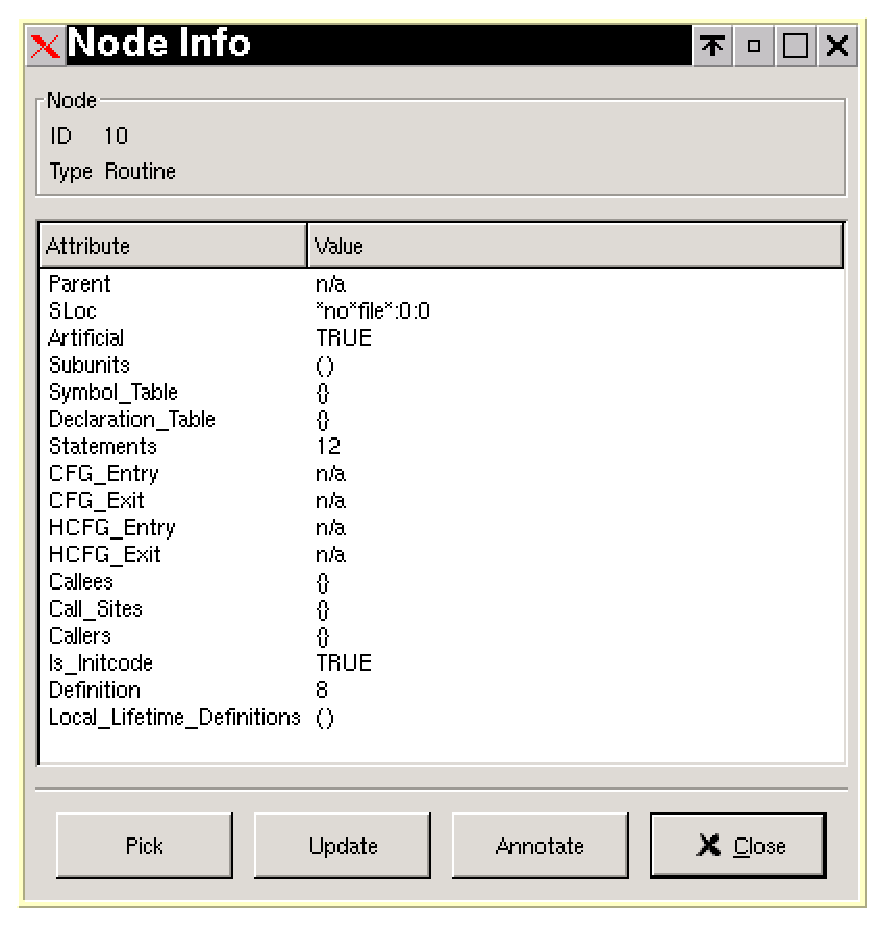
\includegraphics[scale=.4]{tutorial/04-nodeinfo}
   \caption{Node-Info Fenster}
   \label{Node-Info Fenster}
\end{figure}

Wir schlie�en das Nodeinfo-Fenster wieder.

\section{Pin festlegen / �ndern / l�schen}
\index{Pins}

Wir wollen uns nun eine Ansicht des Graphen f�r ein sp�teres schnelles Wiederfinden
merken. Dazu scrollen und zoomen wir in eine f�r uns interessante Position (z.B.
auf Knoten 176 rechts oben im Graphen), klicken mit der rechten Maustaste auf
eine wei�e Fl�che in der Ansicht und w�hlen im Men� \gq{New Pin...} an.
Bei der Frage nach dem Namen des Pins geben wir als Namen z.B. �Kn-176� ein.
Wenn wir nun in eine andere Position scrollen und zoomen, k�nnen wir
durch Aktivieren von �Show� im Popup-Men�, welches bei Auswahl des Knotennamens
mit der Rechten Maustaste in der Pinliste (2) erscheint, wieder zu genau
dieser Ansicht zur�ckspringen.\\
Mit �Rename...� kann der Name des Knotens ge�ndert werden. Wir �ndern den
Knotennamen auf �Interessanter_Knoten�.
Falls wir den Knoten sp�ter einmal l�schen wollen, geht dies mit �Delete�
im Kontextmen�.

\section{Visualisierungsstile �ndern}
\index{Visualisierungsstile �ndern}
Mittels der Visualisierungsstil-Auswahl (4) k�nnen wir die Art der Darstellung
der Knoten �ndern. Probeweise �ndern wir die Darstellung in der Combobox einmal
auf �Plain�. Wir k�nnen nun einmal im Graph herumzoomen und scrollen, um
die Unterschiede zu sehen.
Nun wechseln wir aber wieder zur�ck zum Default-Stil.

\section{Selektionen bearbeiten und markieren}
\index{Selektionen!bearbeiten und farbig markieren}

Wir springen nun zu unserem Pin �Interessanter Knoten�, und zoomen und
scrollen ggf. so, da� wir ca. 8 Knoten bei einer
Zoomstufe von 70 Prozent auf dem Bildschirm haben.\\

Nun klicken wir auf den Knoten Nr. 176 (rechts oben
in der Matrix) mit der linken Maustaste.\\

Der Knoten wird farbig markiert. Wir k�nnen sehen, da� in der Selektionsliste
(3) in der Zeile �Default� der angew�hlte Knoten auftaucht.
Wann immer wir mit der Maus Selektionen manipulieren, so bezieht sich
diese �nderung auf diejenige Selektion in der Liste, bei der in der
Spalte �Active� ein �Yes� steht, die aktive Selektion.\\

Mit gedr�ckter Shift-Taste w�hlen wir noch zwei andere Knoten aus.
Nun halten wir die Shift-Taste und ziehen mit gedr�ckter linker Maustaste
einen Rahmen �ber alle bis auf die unteren zwei Knoten.
Wenn wir loslassen, k�nnen wir feststellen, da� GIANT den momentanen
Status (Selektiert oder nicht) aller Knoten im Rahmen umgekehrt hat.\\

Wenn wir einen Rahmen ohne gedr�ckte Tasten ziehen, werden alle bisherigen
Knoten in der Default-Selektion entselektiert. Wir ziehen nun einen Rahmen
�ber die oberen beiden Knoten. Diesen wollen wir nun die unteren beiden
Knoten hizuf�gen. Dies geschieht durch Anklicken dieser beiden Knoten mit
gedr�ckter Shift-Taste. Alternativ k�nnte auch ein Rahmen mit gedr�ckter
Shift-Taste gezogen werden.\\

Nun ziehen wir einen Rahmen mit der Maus �ber alle Knoten im Fenster
bei gedr�ckter Ctrl-Taste. Wir k�nnen sehen, da� GIANT hier alle
Knoten im Rahmen markiert, im Gegensatz zur Umkehrung des Selektionsstatus
bei Verwendung der Shift-Taste.\\

Zu guter Letzt ziehen wir nochmals einen Rahmen ohne gedr�ckte Tasten �ber
die oberen vier Knoten.\\

Das Selektieren von Kanten funktioniert v�llig analog zum Selektieren der
Knoten.\\

Durch den Rahmen haben wir nun eine gewisse Anzahl von Knoten und Kanten
in der Default-Selektion sichtbar in (3).
Wir duplizieren nun diese Auswahl durch Ausw�hlen von �Duplicate� im Kontextmen�
nach Dr�cken der rechten Maustaste �ber �Default� in der Selektionsliste (3).
Als Namen w�hlen wir �Neu�.\\

Nun wollen wir die Selektion �Neu� farbig markieren. Wir w�hlen dazu in
(3) im Kontext-Men� dieser Selektion �Highlight - Color 1� an.
Wir k�nnen nun sehen, da� die Selektion farbig markiert wurde. (Siehe Bild \ref{Graphenfenster mit rot hervorgehobenem Graph})\\

Durch Ausw�hlen von �Select All� oder �Select Nothing� bei Rechtsklick auf ein
St�ck von Knoten oder Kanten leeren Hintergrund des Anzeigefensterinhaltes k�nnen
alle Knoten und Kanten markiert oder entmarkiert werden.\\

\begin{figure}[h!]
   \centering
   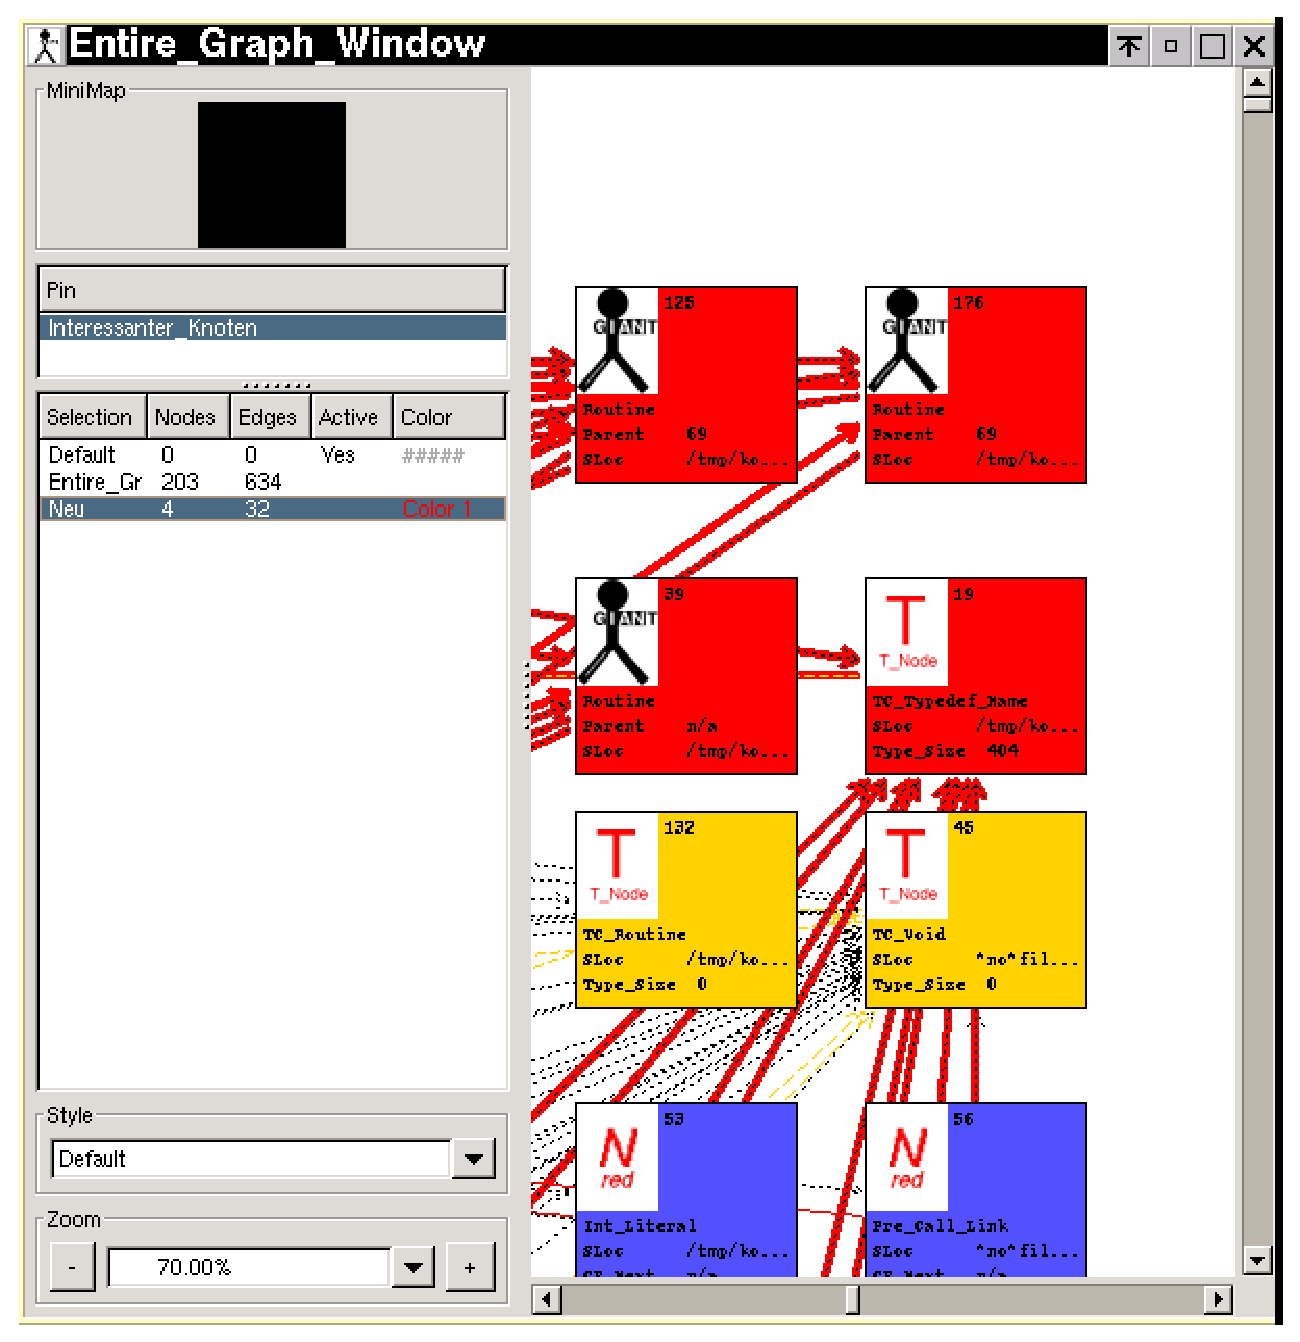
\includegraphics[scale=.5]{tutorial/05-selection-color}
   \caption{Graphenfenster mit rot hervorgehobenem Graph}
   \label{Graphenfenster mit rot hervorgehobenem Graph}
   \clearpage
\end{figure}

\index{Selektionen!anzoomen}
Wenn wir nun im Kontextmen� der Selektion �Zoom to Selection� ausw�hlen,
zoomt und scrollt GIANT so in den Graph hinein, da� alle Knoten der
Selektion sichtbar sind.\\

Mit unserem neu erworbenen Wissen erstellen wir nun eine Selektion
mit der Vierergruppe Knoten unten rechts im Graphen und nennen
sie �vier�. Nun w�hlen wir im Kontextmen� dieser Selektion
�Delete� aus und wir sehen, da� die Knoten noch da sind, die Selektion
aber gel�scht wurde.
Nun erstellen wir nochmals eine Selektion mit dem Namen �neu2�,
w�hlen diesmal �Delete with Content� aus.
GIANT hat nun die Knoten nebst ihrer Kanten aus dem Graph gel�scht.\\

\index{Mengenoperation}

Nun zu einer Mengenoperation:
Auf der Selektion �Neu� in (3) w�hlen wir nun �Set Operation� aus.
Es erscheint der Set Operation Dialog. Wir w�hlen
(siehe Bild \ref{Set Operation Dialog f�r Mengenoperationen}) \\

�Left Source = Entire_Graph�\\
�Operation = Difference�\\
�Right Source = Neu�\\
�Target = Differenzmenge�\\
aus.

\begin{figure}[h!]
   \centering
   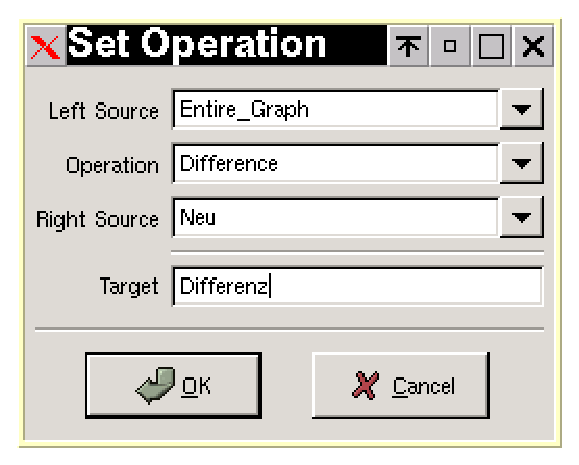
\includegraphics[scale=.5]{tutorial/06-set-operation}
   \caption{Set Operation Dialog f�r Mengenoperationen}
   \label{Set Operation Dialog f�r Mengenoperationen}
\end{figure}
\clearpage

Nun bildet GIANT die Differenz zwischen den beiden Mengen �Entire_Graph�
(also dem Gesamtgraphen) und der Menge �Neu�, die neue Menge heisst
�Differenzmenge�. Man kann sehen, wie sich die Kantenzahlen
unterscheiden.\\
Nun w�hlen wir auf �Differenzmenge� den Men�punkt �Set Active� aus.
Diese Menge ist nun die aktive Selektion. 
Wir k�nnen nun sehen, da� alle Knoten im Graphen, die zur Menge
geh�ren, markiert sind. Mit gedr�ckter Shift-Taste k�nnen wir nun
z.B. Knoten zur Selektion hinzuf�gen oder aus ihr entfernen.

Nachdem wir einige Knoten ausgew�hlt haben, w�hlen wir wieder die
�Default� Selektion als Aktiv an.\\

Unsere Sekektion �Differenzmenge� mit ihren ausgew�hlten Knoten
f�gen wir nun als eigenst�ndigen Subgraphen in GIANT ein, dies
passiert durch Ausw�hlen von �Insert as Subgraph� in ihrem
Kontextmen�. Wie wir sehen, erscheint sie nun im Hauptfenster
in der Subgraph-Liste.\\

\section {Verschieben von Knoten, Platz schaffen}
\index{Platz schaffen}

Wir k�nnen mit der linken Maustaste durch Drag and Drop Knoten
verschieben. Es kann vorkommen, da� Knoten aufeinander liegen,
sie k�nnen dann damit auseinandergeschoben werden.\\

Durch Klick mit der rechten Maustaste auf einen freien Platz im
Anzeigeinhalt des Graphenfensters k�nnen wir im Popup-Men�
�Make Room� anw�hlen. Durch diese Operation werden die
Knoten rund um den freien Platz auseinandergeschoben, je n�her
desto weiter. Bild \ref{Make-Room-Result} zeigt das Ergebnis einer
solchen Operation.

\begin{figure}[h!]
   \centering
   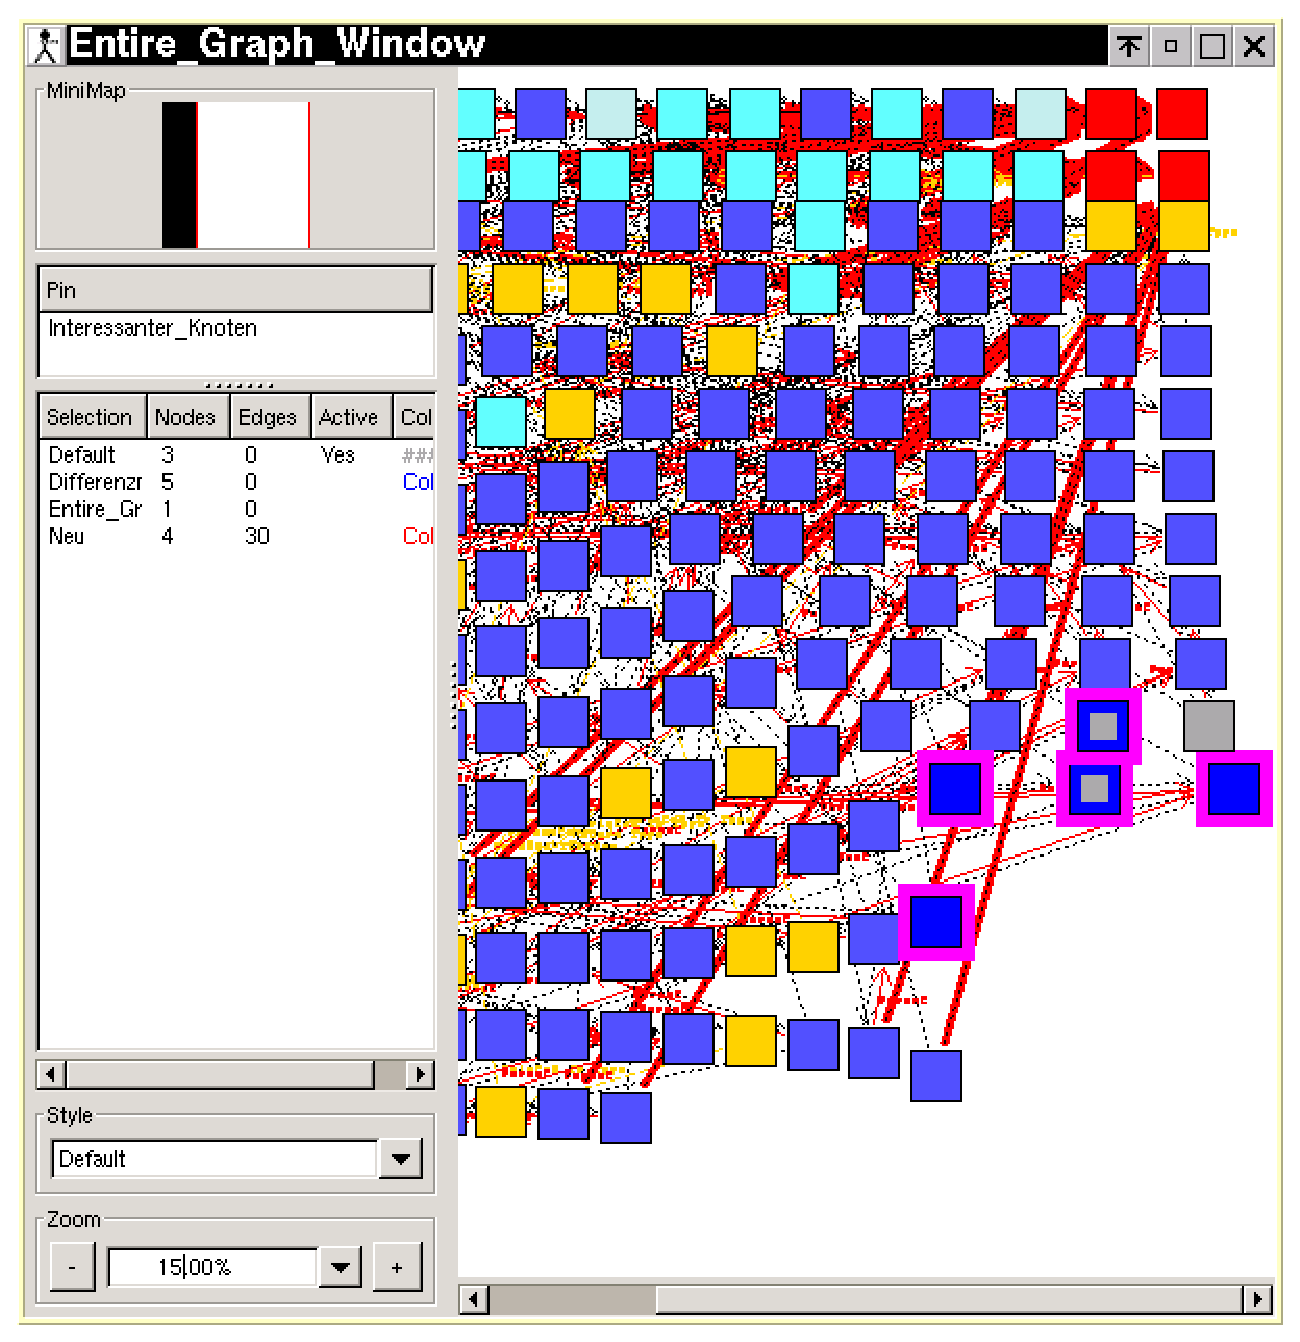
\includegraphics[scale=.5]{tutorial/08-make-room}
   \caption{Resultat von Platz schaffen}
   \label{Make-Room-Result}
\end{figure}


\section{Mehrere Fenster}

Durch Ausw�hlen von �Window - New� erschaffen wir ein neues leeres
Fenster. Dieses wird in der Fensterliste im Hauptfenster angezeigt.
Das Fenster heisstr �Unknown�, wir �ndern seinen Namen durch
Anw�hlen von �Rename� auf im dazugeh�rigen Popup-Men� in der
Liste auf �Testfenster�.\\
Wir schlie�en nun unser eingangs erstelltes Fenster �Entire_Graph_Window�
durch Klick auf den Close-Button rechts oben und speichern es bei der
erscheinenden Sicherheitsabfrage.
Mittels �Open� in seinem Popup-Men� k�nnen wir es bei Bedarf wieder �ffnen.\\

\begin{figure}[h!]
   \centering
   \includegraphics[scale=.5]{tutorial/07-main-window}
   \caption{Hauptfenster}
\end{figure}

\index{Teilgraphen!in Fenster einf�gen}

Nun wollen wir unseren Teilgraphen in das neue Testfenster einf�gen.
Dazu w�hlen wir im Hauptfenster auf dem erstellten Subgraphen im
Popup-Men� �Insert as Selection�. GIANT fordert uns auf, in den leeren
Anzeigeinhalt des Fensters zu klicken, dort wird der Subgraph als Selektion
eingef�gt.\\

Wir �ffnen nun wieder unser erstes Fenster �Entire_Graph_Window�durch
Ausw�hlen von �Open� auf seinem Popup-Men�.\\

Wir w�hlen im Kontextmen� des Subgraphen im Hauptfenster aus\\
�Highlight - Color 2� und k�nnen sehen, da� unsere
Selektion in beiden Fenstern hervorgehoben wurde. Mittels
�Unhighlight in alle Windows� l��t sich die Markierung r�ckg�ngig
machen.\\

Wir schlie�en und speichern das �Testfenster�.

\section{Layouts}
\index{Layouts}

Mittels des oben erw�hnten �Select All� entmarkieren wir alle Knoten in
unserem verbleibenden Fenster. Wir sorgen daf�r, da� im Fenster ca.
die H�lfte des Anzeigeinhaltes frei ist.
Wir w�hlen durch Ziehen mit der Maus ca. 10-15 Knoten im linken
oberen Teil des Graphen aus und w�hlen
dann in der Selektionsauswahlliste auf der aktiven �Default� Selektion
�Apply Layout� aus.\\


Mittels �Matrix Layout� l��t sich der Inhalt des Fensters in
eine Matrixform bringen. Wir w�hlen diese Option im Tab aus
(siehe Bild \ref{Matrix-Layout}).

\begin{figure}[h!]
   \centering
   \includegraphics[scale=.6]{tutorial/09-matrix-layout}
   \caption{Apply Layout}
   \label{Matrix-Layout}
\end{figure}

Nach Klick auf �OK� klicken wir an eine leere Stelle im Anzeigefenster-
Inhalt, dies zeigt GIANT, wo die umorganisierten Knoten platziert
werden sollen.
Ein m�gliches Resultat wird in Bild \ref{Matrix-Layout2} gezeigt.

\begin{figure}[h!]
   \centering
   \includegraphics[scale=.55]{tutorial/10-matrix-layout2}
   \caption{Ergebnis des Matrix-Layouts}
   \label{Matrix-Layout2}
\end{figure}


Wir w�hlen im Popup-Men� des Knoten rechts oben �Show Info�
aus und merken uns den oben im Fenster angezeigten numerischen Wert �ID�
des Knotens.

Nun w�hlen wir ca. 5 * 5 Knoten in der rechten oberen Ecke des Graphen
durch Ziehen mit der Maus aus, einer dieser Knoten sollte der mit der
bekannten ID sein. Vorher sollten wir daf�r sorgen, da�
auch noch gen�gend freier Platz im Fenster sichtbar ist.\\



Wir w�hlen dann in der Selektionsauswahlliste auf der aktiven �Default�
Selektion �Apply Layout� aus. In das Feld �Root Node ID� tragen wir
die ID des Knotens ein.
In der Liste �Class Sets� w�hlen wir �parent_edge_class_set�, �empty_class_set�
und �normal_class_set� aus. Dies sind die Klassenmengen, die f�r das
Layout ber�cksichtigt werden. Nun ist noch ein Klick an die Position
des Wurzelknotens im Anzeigefenster n�tig, und das Layout wird berechnet
und angezeigt.

\section{Benachbarte Knoten}

Mittels des Men�punktes �Scripts - Get Adjacent Nodes� k�nnen die
benachbarten Knoten eines Knotens in eine Knotenmenge eingef�gt werden.
Wir f�hren dies mit einem beliebigen Knoten aus und k�nnen dies
auch anhand der Knotenzahlen �berpr�fen.

\section{Annotieren}
\index{Annotieren}
Knoten k�nnen durch Klick auf �Annotate� im Knoteninformationsfenster
(siehe Bild \ref{Node-Info Fenster}) oder durch Auswahl des Punktes
�Annotate� im Knoten-Popup-Fenster annotiert werden.

Nach der Auswahl von �Annotate� �ffnet sich das Knoten-Annotationsfenster
(siehe Bild \ref{Node Annotation Window}). Hier kann ein Kommentar zum
Knoten eingef�gt werden, der mit gespeichert wird. Durch Delete
kann der Kommentar wieder gel�scht werden.\\
Annotationen werden nur dann auf Festplatte gespeichert, wenn wir im
Hauptmen� �Project - Save� oder �Project - Save As..� ausw�hlen, nicht
jedoch, wenn nur einzelne Fenster gespeichert werden.

\begin{figure}[h!]
   \centering
   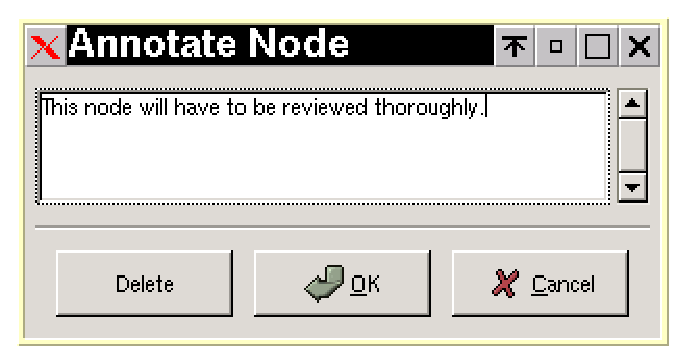
\includegraphics[scale=.55]{tutorial/11-annotation}
   \caption{Knoten-Annotationsfenster}
   \label{Node Annotation Window}
\end{figure}

Nach dem Annotieren wird der Benutzer bei gen�gend gro�er Zoomstufe
durch ein kleines \gq{Dokument}-Symbol auf die Annotation
aufmerksam gemacht. (siehe Bild \ref{Node Annotation Window2})

\begin{figure}[h!]
   \centering
   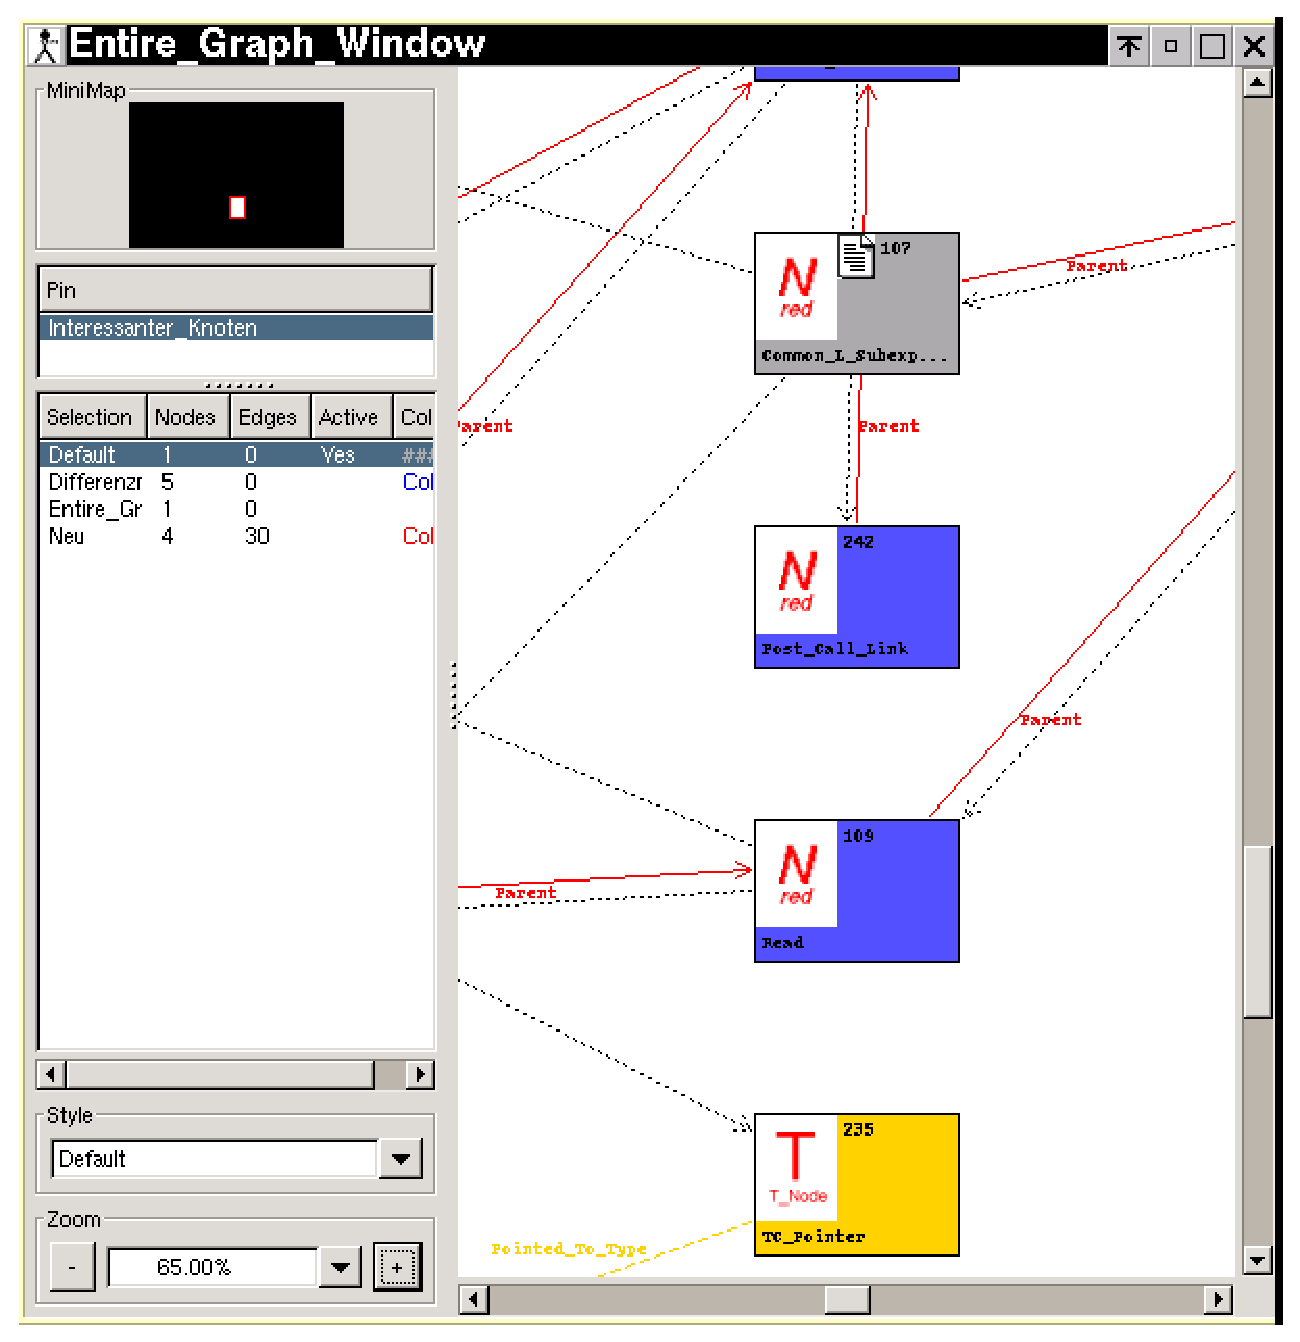
\includegraphics[scale=.55]{tutorial/12-annotation2}
   \caption{Annotierter Knoten Nr. 107}
   \label{Node Annotation Window2}
\end{figure}

\section{Fenster speichern}
\index{Fenster speichern}

Wir wollen nun alle unsere �nderungen im Fenster speichern. Dazu
w�hlen wir im Hauptfenster im Popup-Men� des Fensters �Save� aus,
das Fenster ist nun gespeichert und erscheint beim n�chsten Laden
der Projektdatei auch in der Liste in genau dem Zustand
(Knotenpositionen etc.), in dem wir es gespeichert haben.
Lediglich Annotationen werden nicht gespeichert.

\section{HPG darstellen}

Durch Anw�hlen von �Scripts - Open HPG� im Men� des Hauptfensters
von GIANT k�nnen wir ein Graphenfenster mit dem hierarchischen Programmgraphen
�ffnen.

\section{Einbinden der GSL in Men�punkte}
\index{GSL!Einbinden in Men�punkte und Kontextmen�s}

Zur Verkn�pfung von GSL-Ausdr�cken mit Men�punkten in den
Popup-Men�s von Knoten bzw. Kanten oder dem Hauptmen� sind folgende
Schritte n�tig:\\

Zuerst erstellen wir die GSL-Datei, welche ggf. den Knoten oder die
Kante als \gq{Parameter} �bergeben bekommt, und speichern diese
im GIANT-Verzeichnis �shared/gsl� ab.\\

N�tig ist auch der Eintrag des Skriptes in der Config-Datei
�etc/global-config.xml� im GIANT-Verzeichnis, hierzu mu� diese 
in einen �GSL.� Setting-Knoten eingetragen werden, n�here Informationen
k�nnen wir leicht dem mitgelieferten Config-File oder Abschnitt
\label{Config-GSL-Context-Scripts} entnehmen, Trennzeichen ist
der Doppelpunkt (�:�).\\
Der Eintrag im Men� mu� dabei dem Filenamen entsprechen, ggf. ergeben
sich dadurch auch Leerzeichen im Filenamen.\\

Soll das Skript im Hauptmen� aufrufbar sein, so f�gen wir seinen Namen in
Knoten �GSL.No_Param� ein. F�r einen kontextabh�ngigen
Aufruf aus einem Fenster (im Popup-Men� auf dem leeren
Hintergrund des Fensters) ist �GSL.No_Param_Context� richtig,
und f�r Knoten- Kanten- Teilgraph- oder Selektionssensitive
Aufrufe sind �GSL.Node_Id_Param�, �GSL.Edge_Id_Param�, �GSL.Subgraph_Param�
oder �GSL.Selection_Param� zust�ndig.


%===============================================================================
% 
% Beschreibung der Funktionen
%
\chapter{Beschreibung der Benutzeroberfl�che}
\label{Beschreibung der Funktionen}

Dieses Kapitel beschreibt, geordnet nach den in GIANT auftretenden Fenstertypen,
alle Buttons, Men�s und Funktionen. Dies ist als Nachschlagewerk �ber
alle Elemente der graphischen Benutzeroberfl�che (GUI) gedacht.

% ==============================================================================
%  $RCSfile: functions.tex,v $, $Revision: 1.24 $
%  $Date: 2003-10-07 14:30:22 $
%  $Author: koppor $
%
%  Description: 
%
%  Last-Ispelled-Revision:
%
% ==============================================================================

\label{Kapitel-Funktionale Anforderungen}

%\section{�ber dieses Kapitel}    
%
%
%Wichtige Informationen zur Persitzenz der Projekte in GIANT,
%welche Informationen jeweils gespeichert werden, finden sich
%im Abschnitt \ref{Project Persistenz der Projekte}.

\section {Kommandozeilenaufruf} \label{fa Starten von GIANT}

Giant kann wie folgt von der Kommandozeile aus gestartet werden:

\begin{enumerate}
 \item{Ohne Parameter:}\\

�./giant�

 \item{Mit Parametern, �[]� bedeutet \gq{optional}, �|� bedeutet \gq{oder}:}\\

�./giant  project-file [-g graph-file] [-e script-file]�\\
�     [-c config-file] | -h | -v�

�project-file� ist der Filename der Projektdatei, �graph-file� der Filename
des IML-Graphen. �script-file� ist eine Datei, die ein GSL Script enth�lt,
da� nach dem Laden bzw. Erzeugen des Projektes Ausgef�hrt wird. �config-file�
ist die optional anzugebende globale Konfigurationsdatei, siehe Abschnitt
\ref{config-allgemeines-punkt2}.

Die Option �-h� steht f�r Hilfe, mit �-v� kann die Programmversion von
GIANT angezeigt werden.\\
Wenn ein Graph-File angegeben wird und �project-file� nicht existiert, wird
ein neues Projekt mit diesem Namen erzeugt.\\

Ein Beispiel f�r den Kommandozeilenaufruf von GIANT ist:\\

�./giant projects/sample.project -g graphs/mygraph.xml�\\

\end{enumerate}

\clearpage
\section {Main Window}

\begin{figure}[h!]
   \centering
   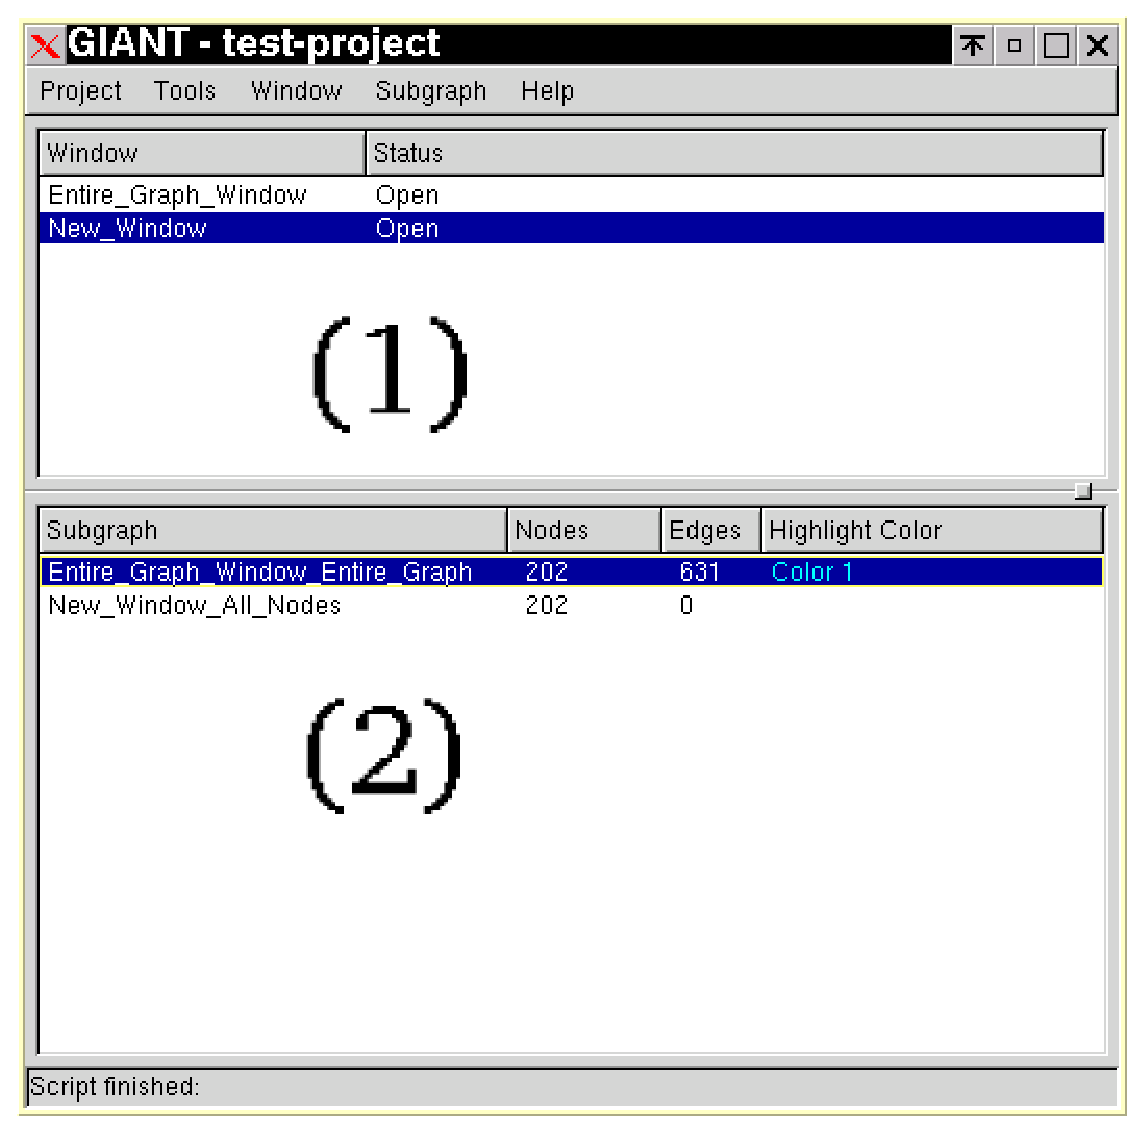
\includegraphics[scale=.75]{gui/main_window}
   \caption{Main-Window}
   \label{Main-Window-Pic}
\end{figure}

\clearpage

%Erg�nzungen by Martin
Jede Instanz von GIANT hat genau ein Hauptfenster. \index{Hauptfenster}
Im Hauptfenster (siehe Abbildung \ref{Main-Window-Pic}) werden die
Anzeigefenster und
IML-Teilgraphen des aktuell ge�ffneten Projektes (siehe  
\ref{Project Persistenz der Projekte}) in Listen angezeigt. 
�ber Popup-Men�s k�nnen IML-Teilgraphen
und Anzeigefenster manipuliert werden.

Im Fenster befinden sich zwei Listen, Window List (1) und
Subgraph List (2).


  \subsection {Titelzeile}
  In der Titelzeile wird \gq{GIANT - <Projektname>} dargestellt.
 
  \subsection {Men�leiste (Main Window)}
  In der Men�leiste befinden sich folgende Eintr�ge:

    \subsubsection {Untermen� Project} \label{Main-Window-Project}
      \begin{enumerate}
         \item {New}\\
         
         Hiermit wird ein neues Projekt angelegt. Ein eventuell bereits ge�ffnetes
         Projekt wird dabei geschlossen, wobei �nderungen auf Nachfrage 
         vorher gespeichert werden.

         \begin{itemize}
         
    \item{GIANT zeigt den Standard-Filechooser-Dialog und fordert den
    Benutzer auf, eine vorhandene IML-Graph Datei auszuw�hlen.}
    
    \item{GIANT zeigt erneut den Standard-Filechooser-Dialog und fordert den
    Benutzer zur Eingabe des Namens der Projektdatei auf. Die Dateiendung wird sp�ter
    von GIANT automatisch gesetzt.}
    
    \item {Der Name der Projektdatei ist
    automatisch auch der Name f�r das Projekt. Das Verzeichnis der
    Projektdatei wird automatisch zum Projektverzeichnis. Existiert die eingegebene Projektdatei bereits, 
    erscheint eine Fehlermeldung.
    Existiert in dem Projektverzeichnis bereits eine andere Projektdatei, so 
    erscheint ebenfalls eine Fehlermeldung.}
        \end{itemize}
    
         \item {Open}\\
         
         �ffnet ein GIANT Projekt. Ein eventuell bereits ge�ffnetes
         Projekt wird dabei geschlossen, wobei �nderungen auf Nachfrage 
         vorher gespeichert werden.
         \begin{itemize}
           \item {War vorher bereits ein Projekt offen, erscheint vorher eine
           Abfrage, ob dieses gespeichert werden soll.}
           \item {GIANT zeigt den Standard-Filechooser-Dialog und fordert
           den Benutzer zur Auswahl einer vorhandenen GIANT-Projektdatei auf.}
         \end{itemize}
         \item {Save}
         
         Speichert ein Projekt in die Verwaltungsdateien im Projektverzeichnis
         der neuen Projektdatei.
         
         \item {Save As...}
         
         Speichert ein Projekt in die Verwaltungsdateien im Projektverzeichnis
         der neuen Projektdatei unter neuem Namen.
         
         \begin{itemize}
          \item{Der Benutzer gibt im Standard-Filechooser-Dialog 
             das neue Projektverzeichnis 
             und den Namen f�r die neue Projektdatei ein, die Dateiendung 
             wird sp�ter von GIANT automatisch gesetzt.}
         \end{itemize}
         
         \item {Info}
         
         Zeigt einen Informationsdialog �ber den Graphen an.
         
         \item {Quit}
         
         Beendet das Programm GIANT.
         
      \end{enumerate}    
      
     \subsubsection {Untermen� Tools}  \label{Main-Window-Tools}
       \begin{enumerate}

          \item {GSL Editor...}
          
          Mit diesem Men�punkt kann ein GSL Script ausgef�hrt werden.
          Es erscheint der Skriptdialog, in den das Skript eingegeben
          werden kann. Es ist auch m�glich, Skripte zu laden oder zu
          speichern. Details hierzu finden sich unter \ref{GUI Anfragedialog}.
          
        \end{enumerate}
        
        
    \subsubsection {Untermen� Window}  
        \begin{enumerate}
          \item {New}\\
          Mit diesem Men�punkt kann ein neues leeres Fenster ge�ffnet werden.
        \end{enumerate}
    \subsubsection {Untermen� Subgraph}  
        \begin{enumerate}
          \item {New}\\
          Mit diesem Men�punkt kann ein neuer leerer IML-Teilgraph erstellt werden.
         \item {Set Operation}\\
          Mit diesem Men�punkt kann eine Mengenoperation auf IML-Teilgraphen
          durchgef�hrt werden, GIANT zeigt dazu den \gq{Set Operation Dialog},
          siehe Abschnitt \ref{Common-Set-Operation-Dialog}.
        \end{enumerate}
        

    \subsubsection {Untermen� Help}  \label{Main-Window-Info}     
       \begin{enumerate}
          \item {About..}\\
          Dieser Men�punkt gibt ein Fenster mit Informationen zur
          GIANT Programmversion und zu den Autoren aus.
        \end{enumerate}
     

  \subsection {Statuszeile}
  \label{Statuszeile}
  \index{Statuszeile}
  Die Statuszeile befindet sich ganz unten im Hauptfenster. In der
  Statuszeile werden Informationen zum aktuellen Zustand von GIANT
  dargestellt.

   \subsection {Window List (1)}
  
   Im Hauptfenster befindet sich zuoberst eine Liste \gq{Window List}, welche
   alle Anzeigefenster des Projektes (offen und geschlossen anzeigt).
   Eine Beschreibung, was alles mit einem Fenster gespeichert wird,
   befindet sich in Abschnitt \ref{Project Persistenz der Projekte}.
   
   \subsubsection {Inhalt Window List}
   \label{WINDOW-LIST}
   
   Window List hat die Spalten \gq{Window} und \gq{Status}. In
   \gq{Window} wird der Name aller Anzeigefenster dargestellt, in
   \gq{Status} befindet sich der Text "Open", wenn das Fenster
   ge�ffnet ist.
    
    \subsubsection {Popup-Men� Window List}
    
    
        Beim Rechtsklick auf Window List �ffnet sich ein 
        Popup-Men� mit folgenden Men�punkten:
        \label{WINDOW-LIST-POPUP}

        \begin{enumerate}
          \item Open\\
             �ffnet ein im Speicher vorhandenes, momentan geschlossenes Fenster.
          \item Close\\
             Schlie�t ein vorhandenes Fenster, es kann wieder ge�ffnet werden.
             Falls das Fenster noch nicht gespeichert wurde, wird eine
             Sicherheitsabfrage durchgef�hrt, ob gespeichert werden soll.
          \item Save Window\\
             Speichert ein Fenster im Projektverzeichnis.
          \item Rename Window\\
             �ndert den Namen eines Fensters, ein entsprechender Dialog erscheint.
          \item Delete Window\\
             L�scht ein Fenster aus dem Projektverzeichnis, es wird auch aus der Window List gel�scht.
        \end{enumerate}
    
  \subsection {Subgraph List (2)}
  \label{GUI Subgraph List}
    
    Unter der Window List befindet sich eine Liste \gq{Subgraph List} mit
    allen IML-Teilgraphen des Projektes.
   
    \subsubsection {Inhalt Subgraph List} 
    
      Subgraph List hat die folgenden Spalten:
      \begin{enumerate}
        \item Subgraph
        \item Nodes
        \item Edges
        \item Color
      \end{enumerate}
    
      In der Spalte Name stehen die Namen der existierenden IML-Teilgraphen,
      in Nodes die Anzahl der Graph-Knoten des jeweiligen IML-Teilgraphen, 
      in Edges die Anzahl der Graph-Kanten und in Highlighted befindet sich
      ein K�stchen in der
      Farbe, die f�r die Hervorhebung des IML-Teilgraphen verwendet wird.
      Bei nicht hervorgehobenen IML-Teilgraphen wird dieses K�stchen
      nicht angezeigt.

    
    \subsubsection {Popup-Men� Subgraph List}
    \label {Popup-Men� Subgraph List}
      Bei einem Rechtsklick auf Subgraph List �ffnet 
      sich ein Popup-Men� mit folgenden Men�punkten:
        \label{SUBGRAPH-LIST-POPUP}
        \begin{enumerate}
          \item Highlight (Men�)
            \begin{enumerate}
              \item Color 1
              \item Color 2
              \item Color 3\\
              Mit diesen drei Men�punkten kann der angew�hlte IML-Teilgraph
              in allen Fenstern in der ausgew�hlten Farbe markiert werden.
            \end{enumerate}
          \item Unhighlight In All Windows\\
             Mit diesen drei Men�punkten kann der angew�hlte IML-Teilgraph
              in allen Fenstern wieder entf�rbt werden, die Markierung also
              entfernt werden.
              
              
          \item Insert as Selection\\
             Mit diesem Men�punkt kann ein IML-Teilgraph als Selektion in ein
             Fenster kopiert werden. Nach Ausw�hlen dieser Funktion ist mit der
             Maus (linke Taste) in das Fenster zu klicken, in das der Subgraph
             eingef�gt werden soll, an eine passende Stelle zu klicken.
          \item Rename
             Mit dieser Funktion kann der Name eines IML-Teilgraphen ge�ndert werden,
             ein entsprechender Dialog erscheint nach der Auswahl dieses Punktes.
          \item Duplicate
             Mit dieser Funktion kann ein IML-Teilgraph dupliziert werden,
             ein Dialog zur Auswahl eines neuen Namens erscheint nach der
             Auswahl dieses Punktes.
          \item Delete
             Mit diesem Men�punkt kann ein IML-Teilgraph nach Sicherheitsabfrage
             gel�scht werden.
        \end{enumerate}   
        Als weitere Men�punkte im Popup-Men� erscheinen die im GIANT-Config-File
        definierten kontextsensitiven GSL-Skripte. Mehr Informationen hierzu finden
        sich in Abschnitt \ref{Config-GSL-Context-Scripts}.

\clearpage
\section {Anzeigefenster} \label{GUI Anzeigefenster}
\index{Anzeigefenster}

  \begin{figure}[!htbp]
     \centering
     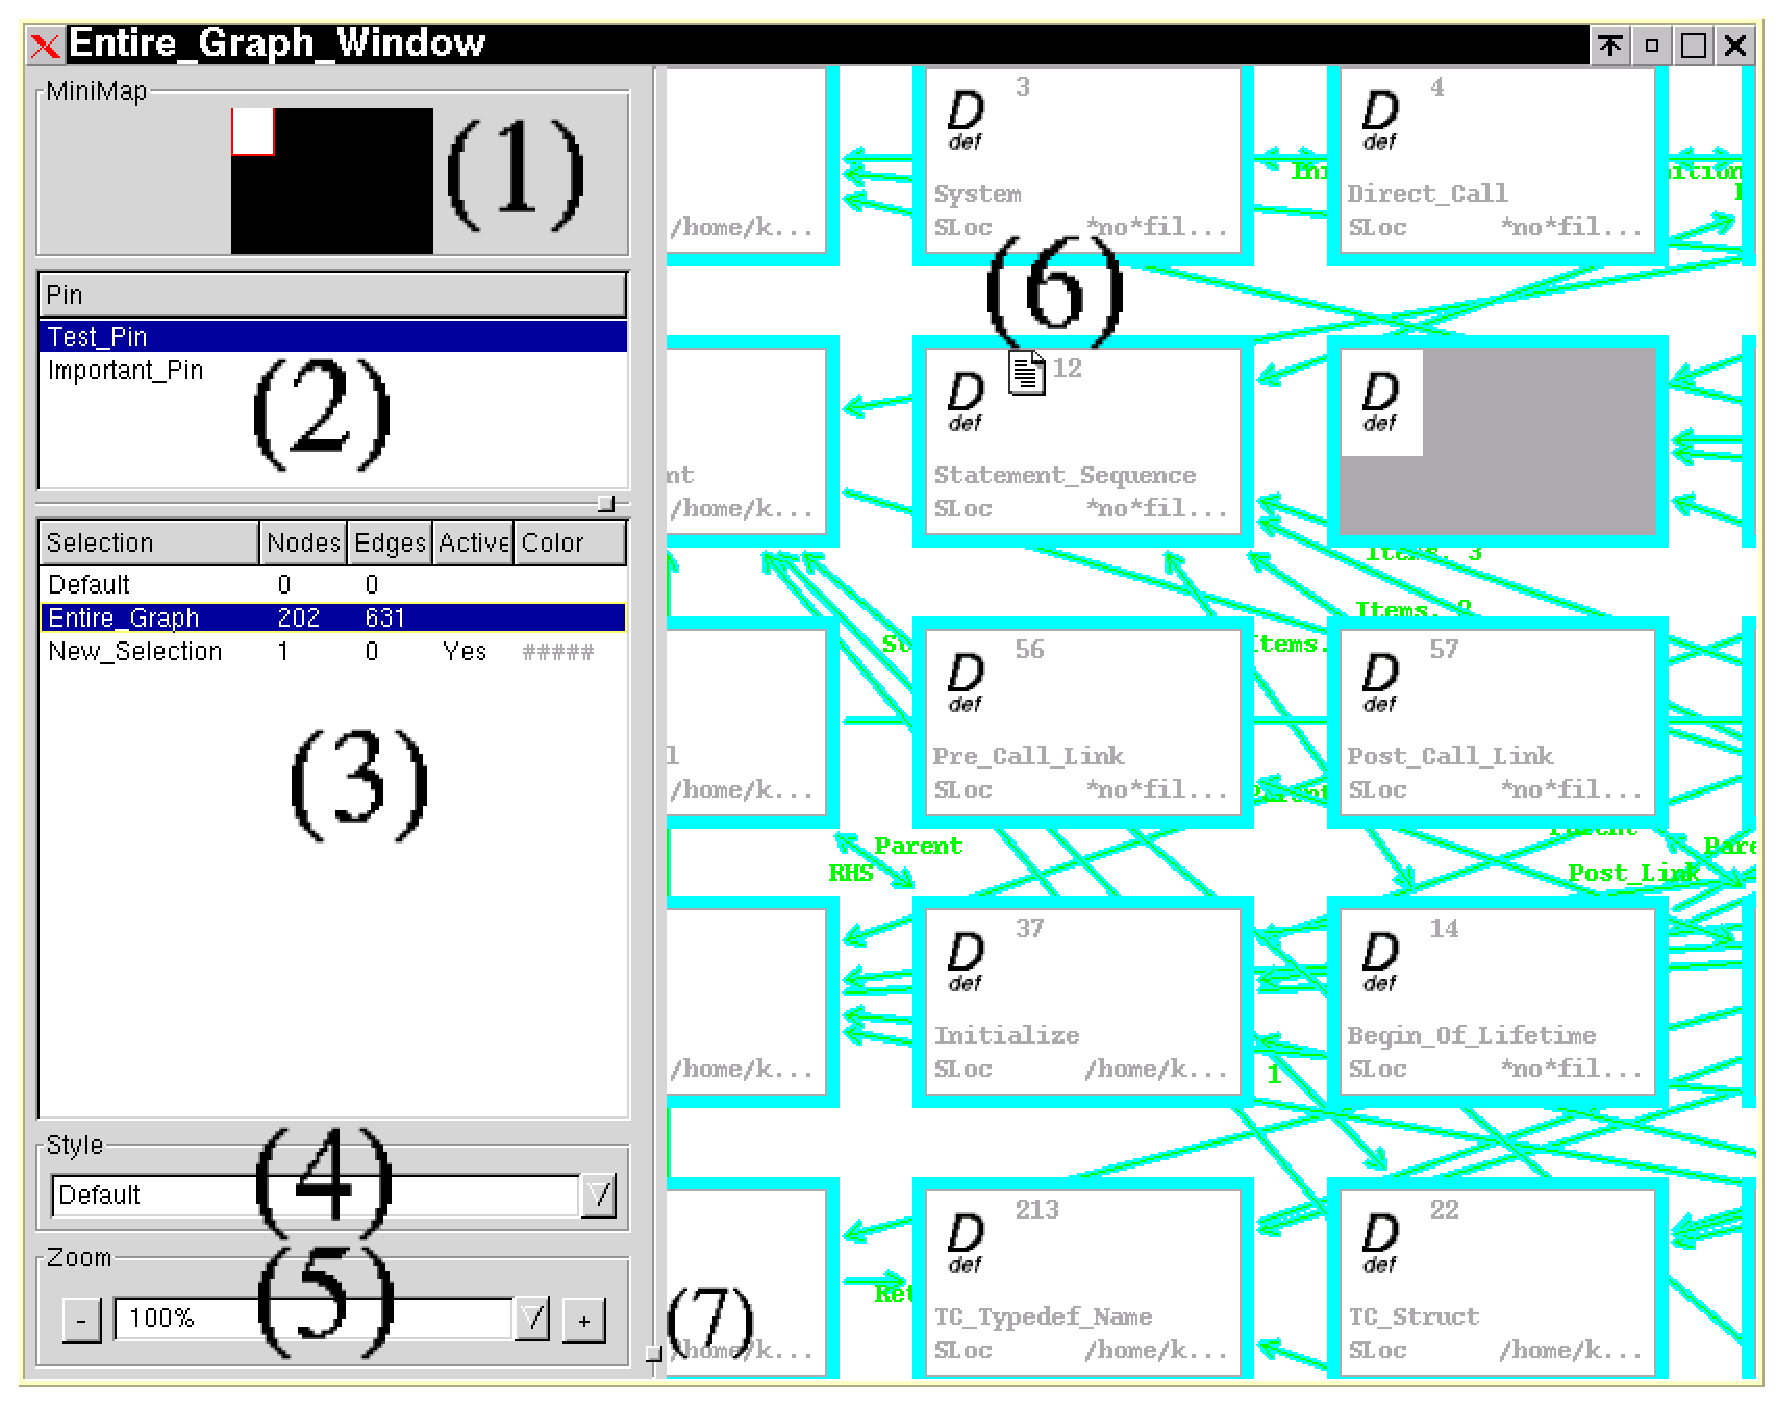
\includegraphics[width=16cm]{gui/visualization_window}
     \caption{Graph-Window}
     \label{Graph-Window-Pic}
  \end{figure}

  Im Programm kann es mehrere Anzeigefenster 
  (siehe Abbildung \ref{Graph-Window-Pic}) geben. 
  

  In Anzeigefenstern (Visualization Windows) werden Teile des IML-Graphen
  visualisiert.  Sie erscheinen im gro�en quadratischen rechten Teil
  (\gq{Vis Pane} (6)) des Fensters. Die Vis Pane enth�lt den Anzeigeinhalt
  des Fensters.  Im linken Teil des Fensters, der Toolbar
  (\gq{Vis Toolbar}) befinden sich untereinander die
  MiniMap (1), Pinliste (2), Selektionsliste (3), die Stilauswahl-Combobox (4) und die
  Zoom-Kontrolle (5). Dieser Teil kann durch Verschieben des entsprechenden
  Buttons (7) unten an der Trennleiste in der Gr��e ver�ndert werden.
  \index{Zoom-Kontrolle}
  \index{Visualisierungsstile!Stilauswahl-Combobox}

 \subsection {MiniMap (1)} \label{GUI Minimap}
 \index{Minimap} 
 
 In der MiniMap wird der Anzeigeinhalt verkleinert dargestellt,
 der Graph wird jedoch nur durch einen grauen Kasten repr�sentiert,
 Knoten sind nicht sichtbar. Die MiniMap wird von einem Rahmen
 umschlossen. Der sichtbare Anzeigeinhalt wird durch einen kleineren
 Rahmen repr�sentiert, der innerhalb der MiniMap durch Mausklicks
 versetzt werden kann. Je nach Zoomstufe ist dieser Rahmen gr��er
 oder kleiner. Wird der Rahmen versetzt, wird der sichtbare Anzeigeinhalt
 in der Vis Pane entsprechend angepasst.\\
 Vergr��ert sich die von Knoten bedeckte Fl�che im Fenster, z.B. durch
 Einf�gen von Teilgraphen, so ver�ndert sich auch die Minimap entsprechend.

  \subsection{Visualisierung der Knoten und Kanten (6)}

    In der Vis Pane werden die Fenster-Knoten und Fenster-Kanten angezeigt.
 
    \subsubsection{Node-Popup-Men�}\label{Node-Popup-Men�}
    
       Wenn auf einem Fenster-Knoten mit der rechten Maustaste geklickt wird, 
    �ffnet sich folgendes Popup-Men�:
    
    \begin{enumerate}
      \item Show Info\\
          Zeigt ein Fenster mit Informationen zum Knoten
      \item Show Source\\
          Zeigt den zum Knoten geh�renden Source Code in einem externen Editorfenster
      \item Annotate...
             Mit diesem Men�punkt l��t sich eine Annotation zu einem Knoten hinzuf�gen,
             �ndern oder l�schen.
             Der Knoten ist dann ggf. graphisch als annotiert gekennzeichnet.
             \label{Change Node Annotation}
             \label{Delete Node Annotation}
             \begin{itemize}
                \item{Der Nutzer f�hrt einen Rechtsklick auf den Knoten aus, den er
                       annotieren will und w�hlt im Popup-Men� \gq{Annotate...} an}
                \item{Im erscheinenden Knotenannotations-Dialog kann der Text der
                      Annotation eingegeben werden und mit OK best�tigt werden.
                      Mittels der Buttons Delete kann die Annotation gel�scht
                      werden, durch Cancel kann die bisherige Annotation beibehalten
                      werden.}
                \item{Nach dem n�chsten Speichern des Projektes ist die Annotation
                      dauerhaft erstellt.}
             \end{itemize}
        \end{enumerate}
        Als weitere Men�punkte im Popup-Men� erscheinen die im GIANT-Config-File
        definierten kontextsensitiven GSL-Skripte. Mehr Informationen hierzu finden
        sich in Abschnitt \ref{Config-GSL-Context-Scripts}.
              Mit diesem Men� k�nnen die GSL-Skripte im Untermen� schnell auf den
              Knoten bezogen ausgef�hrt werden, d.h. ihnen wird die ID des Knotens
              als Parameter �bergeben.
    
    \subsubsection{Background-Popup-Men�} \label{Background-Popup-Men�}
    Wenn in der Vis Pane mit der rechten Maustaste auf eine Stelle
    geklickt wird, an der kein Fenster-Knoten liegt, �ffnet sich das folgende
    Popup-Men�.

    \label{Empty Vis Pane Right click}
    \begin{enumerate}
      \item New Pin\\
         Mittels dieses Men�punktes kann ein neuer Pin (siehe \ref{VIS-PANE-Pins})angelegt werden.
         \begin{itemize} 
             \item{Der Benutzer f�hrt einen Rechtsklick auf den Anzeigeinhalt eines
                Anzeigefensters durch und w�hlt aus dem Popup-Men� 
                (siehe \ref{Empty Vis Pane Right click}) den Eintrag \gq{New Pin} aus.
                Der sp�ter erstellte Pin verweist dann auf die Stelle im Anzeigeinhalt,
                auf die der Rechtsklick durchgef�hrt wurde.}
             \item{Der Benutzer gibt im aufgehenden Texteingabedialog einen
                zul�ssigen Namen f�r den neuen Pin ein und best�tigt mit OK}
             \item{GIANT speichert die aktuelle Zoomstufe und die Position des sichtbaren
                Anzeigeinhaltes in einem neuen Pin.}
         \end{itemize}
      \item Make Room\\
        Mittels dieses Men�punktes k�nnen Knoten auseinandergeschoben werden,
        um Platz zu schaffen.
        \begin{itemize}
         \item{Der Nutzer f�hrt einen Rechtsklick auf eine leere Stelle des
         sichtbaren Anzeigeinhalts in einem Anzeigefenster durch und w�hlt im erscheinenden
         Popup-Men� \gq{Make Room} an}
         \item{GIANT zeigt in der Statuszeile im Hauptfenster 
               \gq{Select position in display window}.
                Der Benutzer gibt den Punkt um den herum die Fenster-Knoten (und damit
                automatisch auch die Fenster-Kanten) auseinander geschoben werden
                 sollen �ber den Fadenkreuzcursor vor.}
         \item{GIANT zeigt einen Dialog an, in dem der Benutzer ausw�hlt, um welchen 
               Betrag die Fenster-Knoten auseinander geschoben werden sollen.
               Der Benutzer w�hlt einen geeigneten Betrag aus und best�tigt mit OK. }    
         \item{GIANT schiebt die Knoten entsprechend auseinander.}
        \end{itemize}
        \item Select All\\
           Bei Auswahl dieses Men�punktes werden alle Knoten im Fenster selektiert.
        \item Select Nothing\\
           Bei Auswahl dieses Men�punktes wird bei allen Knoten im Fenster die
           Selektierung aufgehoben.
        Als weitere Men�punkte im Popup-Men� erscheinen die im GIANT-Config-File
        definierten kontextsensitiven GSL-Skripte. Mehr Informationen hierzu finden
        sich in Abschnitt \ref{Config-GSL-Context-Scripts}.
    \end{enumerate}
    
    \subsubsection{Kanten-Popup-Men�} \label{Kanten-Popup-Men�}
    Wenn in der Vis Pane mit der rechten Maustaste auf eine Kante
    geklickt wird, �ffnet sich ein Popup-Men�:
%*     \begin{itemize}
%*       \item Zoom to edge\\
%*         Dieser Men�punkt zoomt so, da� die gew�hlte Kante gut im Anzeigefenster
%*       sichtbar ist.
%*     \end{itemize}
        Als Men�punkte im Popup-Men� erscheinen die im GIANT-Config-File
        definierten kontextsensitiven GSL-Skripte. Mehr Informationen hierzu finden
        sich in Abschnitt \ref{Config-GSL-Context-Scripts}.
              Mit diesem Men� k�nnen die GSL-Skripte im Untermen� schnell auf die
              Kante bezogen ausgef�hrt werden, d.h. ihnen wird die ID der Kante
              als Parameter �bergeben.

  \subsection{Pins (2)} \label{VIS-PANE-Pins}
  \index{Pins}

    In der Pinliste (\gq{Pin List}) k�nnen Pins angesprungen oder ver�ndert werden.

    Im Popup-Men� der Pinliste befinden sich folgende Men�punkte:
    
    \begin{enumerate}
      \item Show\\
            Mittels dieses Men�punktes kann der sichtbare Anzeigeinhalt gem�� den im Pin gespeicherten
            Informationen gesetzt werden.
      \item Rename\\
            Mittels dieses Men�punktes kann der Name des Pins ge�ndert werden, ein
            entsprechender Dialog erscheint. 
      \item Delete\\
            Mittels dieses Men�punktes kann der Pin aus der Pinliste gel�scht werden.
    \end{enumerate}

  \subsection{Selektionsauswahlliste (3)} \label{Selektionsauswahlliste}
    Die Selektionsauswahlliste hat die Spalten \gq{Name} mit dem Namen der
    Selektion, \gq{Color} mit der Farbe der Selektion und \gq{Active}
    mit \gq{Yes} bei der aktiven Selektion.

    Im Popup-Men� der Selektionsauswahlliste (\gq{Selection List}) befinden
    sich folgende Eintr�ge:

    \begin{enumerate}
      \item Set Active\\
          Mittels dieser Funktion kann eine Selektion zur aktiven Selektion gemacht werden.
      \item Highlight (Men�)\\
        Diese Funktion dient zum Hervorheben von Selektionen innerhalb eines
        Anzeigefensters.
        War bereits eine andere Selektion mit der vom Benutzer gew�hlten
        Farbe hervorgehoben (die Farbe, welche im Popup-Men� der
        Selektionsauswahlliste unter \gq{Highlight Selection} gew�hlt wurde,
        so ist diese Selektion nicht mehr hervorgehoben.
        \begin{enumerate}
         \item Color 1\\
          Hebt in der im Config-File definierten Farbe 1 hervor
         \item Color 2\\
          Hebt in der im Config-File definierten Farbe 2 hervor
         \item Color 3\\
          Hebt in der im Config-File definierten Farbe 3 hervor
        \end{enumerate}
        Der Benutzer startet die Funktion mit einem Rechtsklick 
        auf die gew�nschte Selektion in der Selektionsauswahlliste
        und w�hlt im zugeh�rigen Popup-Men� das Untermen�
        \gq{Highlight Selection} und dort die gew�nschte Farbe aus.
        GIANT hebt die Selektion mit der ausgew�hlten Farbe hervor.
      \item Unhighlight Selection\\
        Diese Funktion dient dazu, die Hervorhebung von Selektionen innerhalb eines 
        Anzeigefensters aufzuheben.
        Der Benutzer startet die Funktion mit einem Rechtsklick 
        auf die gew�nschte Selektion in der
        Selektionsauswahlliste und w�hlt im zugeh�rigen Popup-Men� den Eintrag
        \gq{Unhighlight Selection} aus.
      \item Apply Layout\\
          Mittels dieser Funktion k�nnen Selektionen innerhalb
          eines Anzeigefensters layoutet werden.
          Die verf�gbaren Layoutalgorithmen sind in Kapitel 
          \gq{Layoutalgorithmen} beschrieben.
          \begin{itemize}
           \item{Der Benutzer w�hlt aus der Selektionsauswahlliste (siehe
            \ref{Selektionsauswahlliste}) die Selektion aus, deren
            Fenster-Knoten layoutet werden sollen. Hierzu f�hrt er einen
            Rechtsklick auf die Selektion durch und w�hlt im Popup-Men� den
            Eintrag \gq{Layout Selection} aus.}
           \item{GIANT zeigt einen Dialog zur Auswahl und Konfiguration des
            gew�nschten Layoutalgorithmus 
            (siehe \ref{Layoutalgorithmen-Dialog}). Der Benutzer w�hlt
            in diesem Dialog den gew�nschten Layoutalgorithmus aus.}
          \end{itemize}
      \item Set Operation\\
            Zus�tzlich zu den M�glichkeiten der Anfragesprache GSL (siehe Kapitel
            \ref{GIANT Scripting Language}) kann der Benutzer
            die g�ngigen Mengenoperationen, wie Mengenvereinigung, Schnitt und Differenz,
            auch direkt �ber einen entsprechenden Dialog 
            (siehe \ref{Common-Set-Operation-Dialog}) ausf�hren, welcher mit dieser
            Funktion aufgerufen werden kann.\\
      \item Insert As Subgraph\\
           Dieser Men�punkt leitet einen neuen IML-Teilgraphen aus einer
           Quell-Selektion ab.
           \begin{itemize}
             \item{Der Benutzer f�hrt einen Rechtsklick auf die Quell-Selektion in
                   der Selektionsauswahlliste aus
                   und w�hlt im Popup-Men� den Eintrag 
                   \gq{Create New IML Subgraph from This Selection} aus.}
             \item{GIANT zeigt den allgemeinen Texteingabedialog
                   an. Der Benutzer gibt einen Namen f�r den neu zu erstellenden IML-Teilgraphen
                   ein und best�tigt mit OK.
                   Gibt der Benutzer hier keinen Namen ein, so vergibt GIANT automatisch 
                   einen Namen.}
           \end{itemize}
      \item Rename\\
           Mit dieser Funktion kann der Name einer Selektion ge�ndert werden, GIANT zeigt
           einen entsprechenden Dialog.
      \item Duplicate\\
           Mit dieser Funktion kann eine Selektion dupliziert werden, GIANT fragt in einem
           entsprechenden Dialog nach dem Namen der neuen Selektion.
      \item Zoom To Selection
         Der im Fenster sichtbare Anzeigeinhalts wird durch automatisches Zoomen
         und Scrollen so ver�ndert, dass die ausgew�hlte Selektion vollst�ndig
         sichtbar ist.
      \item Delete\\
           Diese Funktion dient zum L�schen von Selektionen innerhalb eines 
           Anzeigefensters. Hierdurch bleiben die Fenster-Knoten und Fenster-Kanten
           unver�ndert. Die Standard-Selektion (siehe \ref{Standard-Selektion}) kann
           nicht gel�scht werden. Wurde die aktuelle Selektion gel�scht (siehe 
           \ref{Aktuelle Selektion vs Selektionen}), so wird die
           Standard-Selektion zur aktuellen Selektion. Die Fenster-Knoten und
           Fenster-Kanten,  die zur gel�schten Selektion geh�ren, werden nicht
           gel�scht. War die Selektion hervorgehoben, so wird die
           Hervorhebung der Fenster-Knoten und Fenster-Kanten aufgehoben.
           \begin{itemize}
            \item{Der Benutzer startet die Funktion durch Rechtsklick auf die zu
              l�schende Selektion in der Selektionsauswahlliste (siehe 
              \ref{Selektionsauswahlliste}) und w�hlt aus dem Popup-Men� den Eintrag
              \gq{Delete Selection} aus. Falls der Benutzer die Standard-Selektion 
              (siehe \ref{Standard-Selektion}) ausgew�hlt hat, ist der Eintrag
              \gq{Delete Selection} deaktiviert.}
             \item{GIANT l�scht die entsprechende Selektion.}
           \end{itemize}
      \item Delete With Content\\
           Mittels dieser Funktion k�nnen alle Fenster-Knoten und Fenster-Kanten
           einer Selektion aus einem Anzeigefenster gel�scht werden
           (siehe auch \ref{Verhalten beim Entfernen von Fenster-Knoten und 
           Fenster-Kanten}).\\
           Falls die gew�hlte Selektion nicht die Standard-Selektion war,
           ist die Selektion jetzt aus dem Anzeigefenster gel�scht und taucht nicht
           mehr in der Liste �ber die Selektionen auf.
           Wurde die Standard-Selektion (siehe \ref{Standard-Selektion}) 
           gew�hlt, so wird diese nicht aus dem Anzeigefenster gel�scht, sondern
           ist jetzt leer.
           \begin{itemize}
             \item{Der Benutzer f�hrt einen Rechtsklick auf die entsprechende Selektion in der
                   Selektionsauswahlliste durch (siehe \ref{Selektionsauswahlliste})
                   und w�hlt im Popup-Men� den Eintrag \gq{Delete Nodes and Edges
                   of Selection} aus.}
             \item{GIANT zeigt die Sicherheitsabfrage (siehe \ref{Sicherheitsabfrage}) 
                   und fragt nach, ob es die Selektion samt ihrer Fenster-Knoten und 
                   Fenster-Kanten wirklich l�schen soll (\gq{Really delete Selection 
                   from its window including Nodes and Edges?}).
                   Der Benutzer best�tigt mit Yes.}
             \item{GIANT l�scht die Selektion samt allen zugeh�rigen Fenster-Knoten und
                   Fenster-Kanten aus dem entsprechenden Anzeigefenster.
                   Wurde die Funktion f�r die Standard-Selektion
                   (siehe \ref{Standard-Selektion}) ausgef�hrt, so werden die
                   Fenster-Knoten und Fenster-Kanten aus dem Anzeigeinhalt gel�scht, 
                   die Standard-Selektion selbst wird geleert aber nicht gel�scht.} 
           \end{itemize}

            
    \end{enumerate}    


  \subsection{Stilauswahl-Combobox (4)}
  \label{GUI Stilauswahl-Combobox}   

    In der Stilauswahl-Combobox (\gq{Style Chooser}) kann ein 
    Visualisierungsstil (siehe auch \ref{Config Visualisierungsstile})
    ausgew�hlt werden.

  \subsection{Zoom-Kontrolle (5)} \label{GUI Zoom-Kontrolle}  

    Die Zoom-Kontrolle besteht aus folgenden Elementen:
    
  \begin{enumerate}
      \item Button \gq{-} % OK
      \item Combobox mit vorgefertigten Zoom-Werten und Eingabem�glichkeit und Button \gq{OK}.
      \item Button \gq{+} % OK
  \end{enumerate}    

%  In der ComboBox zur Zoom-Kontrolle befindet sich
%  neben den vorgegebenen Zoomstufen \index{Zoomstufe} noch der
%  Eintrag \gq{Whole Graph}, welcher daf�r sorgt, da� der gesamte Graph im
%  Fenster sichtbar ist.
%  Nach Auswahl einer Zoomstufe in der Combobox mu� der Button \gq{OK}
%  geklickt werden.
  
  Mittels der Buttons \gq{+}und \gq{-} kann die Zoomstufe nach oben bzw. unten
  ver�ndert werden, pro Klick ver�ndert sie sich um einen bestimmten Betrag.
 
    \subsection{Scrollen}
    \label{Scrolleisten}
    
    Der sichtbare Anzeigeinhalt kann folgendermassen gescrollt werden:
    \begin{itemize}
      \item{Durch Bewegen des sichtbaren Bereiches in der Minimap mit der Maus}
      \item{Durch Klicken mit der linken Maustaste auf eine leere Stelle des 
            sichtbaren Anzeigeinhalts, festhalten der Maustaste und Bewegen des
            Mauszeigers aus dem Fenster heraus in die entsprechende Richtung
            (oben, unten, links oder rechts).}
    \end{itemize}

\clearpage
\section{Knoten-Informationsfenster} \label{Knoten-Informationsfenster}

    \begin{figure}[!htbp]
       \centering
       \includegraphics[scale=0.6]{gui/node_information_dialog}
       \caption{Node-Info-Window}
       \label{Node-Info-Window-Pic}
    \end{figure}

    In Knoten-Informationsfenstern (siehe Abbildung 
    \ref{Node-Info-Window-Pic}) 
    k�nnen n�here Informationen zu Fenster-Knoten angezeigt werden.\\
    
    Im Knoten-Informationsfenster wird die ID und die Knotenklasse des 
    vom Fenster-Knoten repr�sentierten IML-Knotens dargestellt (1),
    darunter befindet sich die Liste \gq{Attributes} mit den Attributen
    des Knotens (2).\\
    
    Unter der Liste (2) befinden sich nebeneinander die Buttons
    \gq{Pick}, \gq{Update}, \gq{Annotate} und \gq{Close}. 
    \gq{Pick} dient zur Auswahl eines anderen Fenster-Knotens 
    mittels des Fadenkreuzcursors, dazu wird nach Klicken von \gq{Pick}
    ein Fensterknoten angeklickt.\\
    
    \gq{Update} dient zur Aktualisierung der Liste, Annotate �ffnet das
    Knoten-Annotationsfenster (siehe Abschnitt \ref{Knoten Annotations-Dialog}).\\
    
    Die Informationen zu dem ausgew�hlten
    Fenster-Knoten werden dann im Knoten-Informationsfenster dargestellt.\\
    
    Das Knoten-Informationsfenster enth�lt, neben der Anzeige von Knoten-ID
    und Knoten-Typ, die Liste \gq{Attributes}:

    Die Liste Attributes enth�lt die Attribute des Knotens und hat
    zwei Spalten:
    
      \begin{enumerate}
        \item Name  (der Name des Attributes)
        \item Value (der Attributwert)
      \end{enumerate}
    

\clearpage
\section{Skriptdialog} \label{GUI Anfragedialog}

    \begin{figure}[!htbp]
       \centering
       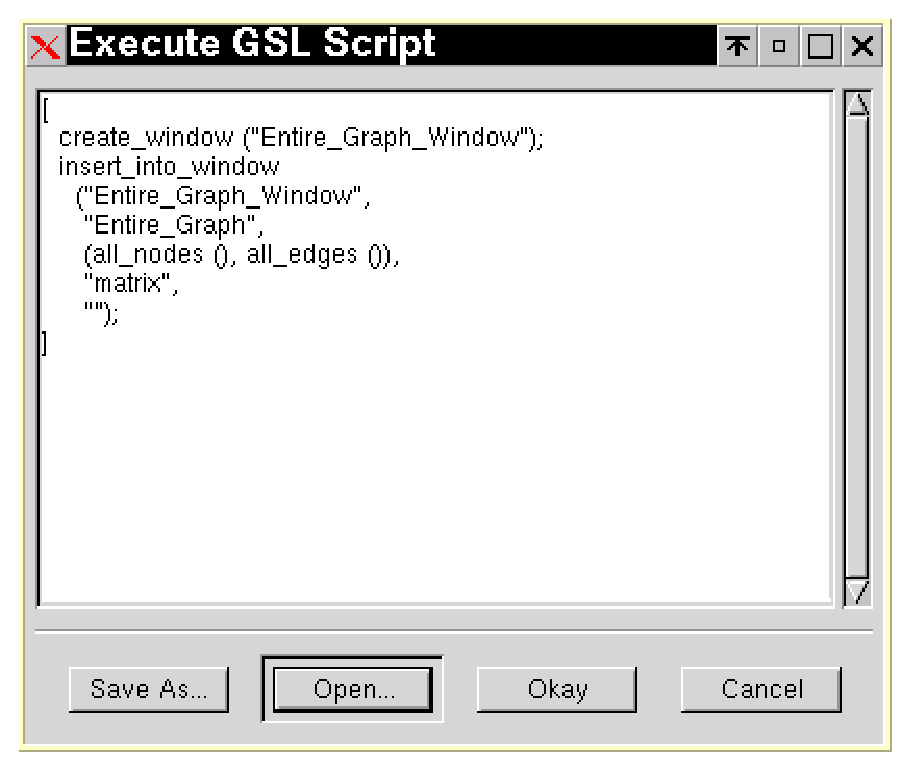
\includegraphics[scale=0.75]{gui/query_dialog}
       \caption{Skript-Dialog}
       \label{Skript-Dialog-Pic} 
    \end{figure}

Der Skriptdialog (siehe Abbildung \ref{Skript-Dialog-Pic})
hat zuoberst ein Textfeld,
in das ein GSL Skript eingegeben werden kann.

Unter Query Text befinden sich folgende Buttons:

      \begin{enumerate}
        \item Open...\\
           Mit diesem Button kann ein auf Festplatte gespeichertes Skript geladen werden.
           Nach Klick auf diesen Button erscheint ein Dateiauswahlfenster, nach Auswahl
           eines Skriptes wird dieses in das Textfeld eingef�gt.
        \item Save As...\\
           Mit diesem Button kann das im Textfeld eingetippte Skript gespeichert werden.
           Nach dem Klick auf diesen Button erscheint ein Dateiauswahlfenster, nach
           Festlegen eines Dateinamens wird das Skript unter diesem Namen gespeichert.
        \item Okay\\
           F�hrt das eingegebene Skript aus.
        \item Cancel
           Schlie�t das Fenster ohne Ausf�hrung oder Speicherung des Skriptes.
      \end{enumerate}
      
\clearpage
\section{Allgemeiner Texteingabedialog}
\label{DIALOG-WINDOW}

    \begin{figure}[!htbp]
       \centering
       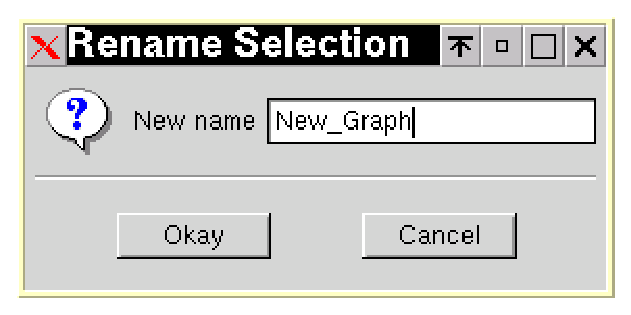
\includegraphics{gui/input_dialog}
       \caption{Dialog-Window}
       \label{Dialog-Window-Pic}
    \end{figure}

Ein allgemeiner Texteingabedialog ist ein Fenster Dialog Window 
(siehe Abbildung \ref{Dialog-Window-Pic}) mit dem
Titel \gq{Input}. Im Fenster ist ein einzeiliges Textfeld
mit einem Prompt-Text, zwei Buttons mit den Beschriftungen \gq{OK}
und \gq{Cancel}.

%\clearpage
\section{Set-Operation-Dialog}
\label{Common-Set-Operation-Dialog}

    \begin{figure}[!htbp]
       \centering
       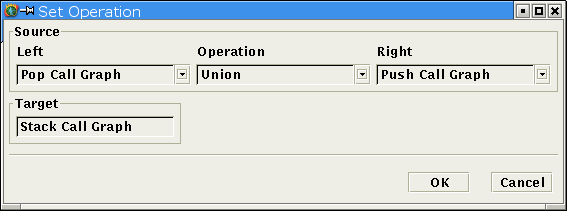
\includegraphics[scale=0.85]{gui/set_operation_dialog}
       \caption{Set-Operation-Dialog}
       \label{Set-Operation-Dialog-Pic}
    \end{figure}


Der Set-Operation-Dialog (siehe Abbildung \ref{Set-Operation-Dialog-Pic}) 
dient dazu, Mengenoperationen �ber 
Selektionen und
IML-Teilgraphen durchzuf�hren.
Die Mengenoperation l�sst sich wie folgt beschreiben:\\
TARGET := LEFT\_SOURCE <Operation> RIGHT\_SOURCE \\


Bestandteile des Dialoges sind:
\begin {enumerate}

 \item Left Source Combobox\\
 Soll eine Mengenoperation f�r Selektionen ausgef�hrt werden, so kann hier eine der
 Selektionen des entsprechenden Anzeigefensters ausgew�hlt werden.\\
 Bei einer Mengenoperation �ber IML-Teilgraphen, werden alle IML-Teilgraphen
 des Projektes angezeigt, von denen dann einer ausgew�hlt werden kann.
 
 \item Operation Combobox\\
 Mengenoperation, die ausgef�hrt werden soll; ausw�hlbar sind: Union, Difference oder Intersection.

 \item Right Source Combobox\\
 Soll eine Mengenoperation f�r Selektionen ausgef�hrt werden, so kann hier eine der
 Selektionen des entsprechenden Anzeigefensters ausgew�hlt werden.\\
 Bei einer Mengenoperation �ber IML-Teilgraphen, werden alle IML-Teilgraphen
 des Projektes angezeigt, von denen dann einer ausgew�hlt werden kann..
 
 \item Target Textfeld\\
 Name der neuen Selektion oder des neuen IML-Teilgraphen als Ergebnis
 der Mengenoperation.
 
 \item Buttons OK und Cancel\\
 Mit den beiden Buttons OK und Cancel l�sst sich die Operation starten bzw.
 der Dialog ohne Ausf�hren der Operation verlassen.
 
\end {enumerate}

 \clearpage
\section {Layoutalgorithmen Dialog}\label{Layoutalgorithmen-Dialog}

    \begin{figure}[!htbp]
       \centering
       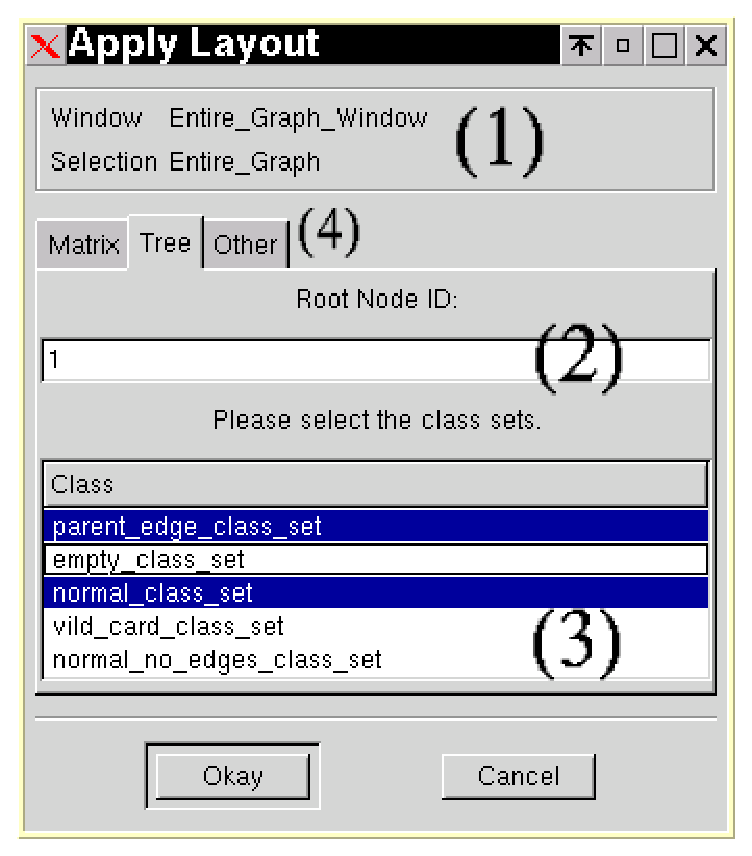
\includegraphics{gui/apply_layout_dialog}
       \caption{Layout-Algorithmen-Dialog}
       \label{Layout-Algorithm-Dialog-Pic}
    \end{figure}

Der Layoutalgorithmen Dialog (siehe Abbildung \ref{Layout-Algorithm-Dialog-Pic}) 
wird �ber Popup-Men�s auf Selektionen aufgerufen und bietet folgende M�glichkeiten:

\begin {enumerate} 
 \item Anzeige der zu layoutenden Selektion mit dem zu layoutenden Fenster (1)
 \item {Auswahl des Layoutalgorithmus}\\
       �ber die Tabs (4) im Fenster kann der Layoutalgorithmus ausgew�hlt werden,
       in der aktuellen Version stehen zur Auswahl: Matrix, Tree Layout,
       Other (f�r sp�tere Erweiterungen).\\
       Das Tree-Layout ordnet die Knoten als Baum an, dessen Wurzel anhand
       der ID des Knotens (welche u.a. mit dem Knoten-Informationsfenster, siehe
        \ref{Knoten-Informationsfenster}, festgestellt
       werden kann) festgelegt wird.\\
       Das Matrix-Layout ordnet die Knoten in einer Matrix an.\\
       
 \item Ggf.\ Eingabefeld f�r die ID des Wurzelknotens bei Treelayouts (2)
 \item {Ggf.\ Auswahl der f�r das Layout der Knoten zu ber�cksichtigenden Klassenmengen (3)
        (class sets, siehe \ref{Config-Klassenmengen} und \ref{Klassenmenge}) bei semantischen Tree-Layouts.}\\
        Nur Klassenmengen, die in der Liste per Mausklick markiert worden sind
        (Mehrfachmarkierungen sind m�glich), werden f�r das Layout
        ber�cksichtigt. Falls keine Klassenmengen angeben wurden,
        werden alle Kanten, {\em auch diejenigen, die nicht im Fenster
        sichtbar sind,} f�r das Layout verwendet.
 \item OK Button
 \item Cancel Button
\end {enumerate}

Nach dem Klicken von OK ist mit der linken Maustaste in ein Fenster auf den
dargestellten Anzeigeinhalt zu klicken (an einer leere Stelle), an dieser
Position wird dann die neu layoutete Selektion eingef�gt.

\clearpage
\section{Dateneingabe}
Beschreibung von verschiedenen GUI Elementen zur Eingabe von Daten.

\subsection{Knoten-Annotations-Dialog}
\label{Knoten Annotations-Dialog}

    \begin{figure}[!htbp]
       \centering
       \includegraphics{gui/annotate_node}
       \caption{Node-Annotation-Dialog}
       \label{Node-Annotation-Dialog-Pic}
    \end{figure}
  
Der Knoten-Annotations-Dialog (siehe Abbildung 
\ref{Node-Annotation-Dialog-Pic}) besteht aus einem Fenster mit einem
Label, welches die ID des Knotens anzeigt, und einem Textfeld f�r den Annotationstext.
Mittels der beiden Buttons Okay und Cancel k�nnen die �nderungen im
Textfeld �bernommen oder verworfen werden. Der Button Delete kann dazu
verwendet werden, das Textfeld zu leeren.
\index{Knoten-Annotationen}


%  \clearpage
\subsection{Platz Schaffen-Dialog}
\label{Platz Schaffen-Dialog}

    \begin{figure}[!htbp]
       \centering
       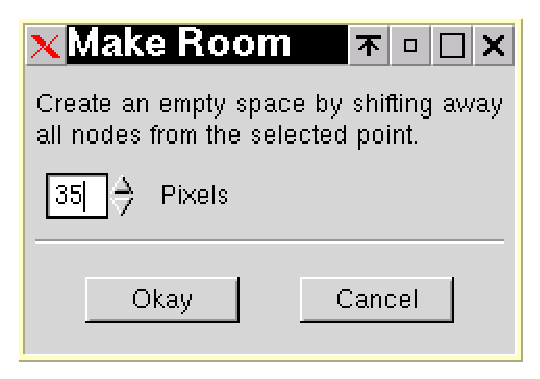
\includegraphics{gui/make_room}
       \caption{Make-Room-Dialog}
       \label{Make-Room-Dialog-Pic}
    \end{figure}

Im Dialogfenster Make Room (siehe Abbildung \ref{Make-Room-Dialog-Pic}) 
wird in einem Textfeld als Zahl 
eingegeben, um wie viel
Pixel die Fenster-Knoten an einer vorher markierten Stelle auseinandergeschoben 
werden sollen.
Mit dem Button Okay kann best�tigt werden, mit dem Button Cancel abgebrochen werden.

\clearpage
\section{Ausgabe von Fehlermeldungen}
\label {GUI Ausgabe von Fehlermeldungen}

    \begin{figure}[!htbp]
       \centering
       \includegraphics{gui/error_dialog}
       \caption{Error-Window}
       \label{Error-Window-Pic}
    \end{figure}

Im Fenster eines allgemeinen Fehlerdialoges (siehe Abbildung \ref{Error-Window-Pic})
befindet sich die Fehlermeldung und ein \gq{OK}-Button, mit dem das
Fenster geschlossen werden kann.. 

\section{Sicherheitsabfrage}\label{Sicherheitsabfrage}
\index{Sicherheitsabfrage}

    \begin{figure}[!htbp]
       \centering
       \includegraphics{gui/confirmation_dialog}
       \caption{Confirmation-Window}
       \label{Confirmation-Window-Pic}
    \end{figure}
    
Eine allgemeine Sicherheitsabfrage (siehe Abbildung \ref{Confirmation-Window-Pic}) 
besitzt einen
Fragetext und die zwei Buttons \gq{Yes} und \gq{No}.
Ggf. kann mit einem Radiobutton festgelegt werden, da� Sicherheitsabfragen
des jeweiligen Types in Zukunft nicht mehr angezeigt werden (z.B. \gq{Do not
show delete confirmations again}).

\clearpage

\section{Auswahl von Dateien}

  \subsection {Der \gq{Standard-Filechooser-Dialog}}
  \label {Standard-Filechooser-Dialog}

    \begin{figure}[!htbp]
       \centering
       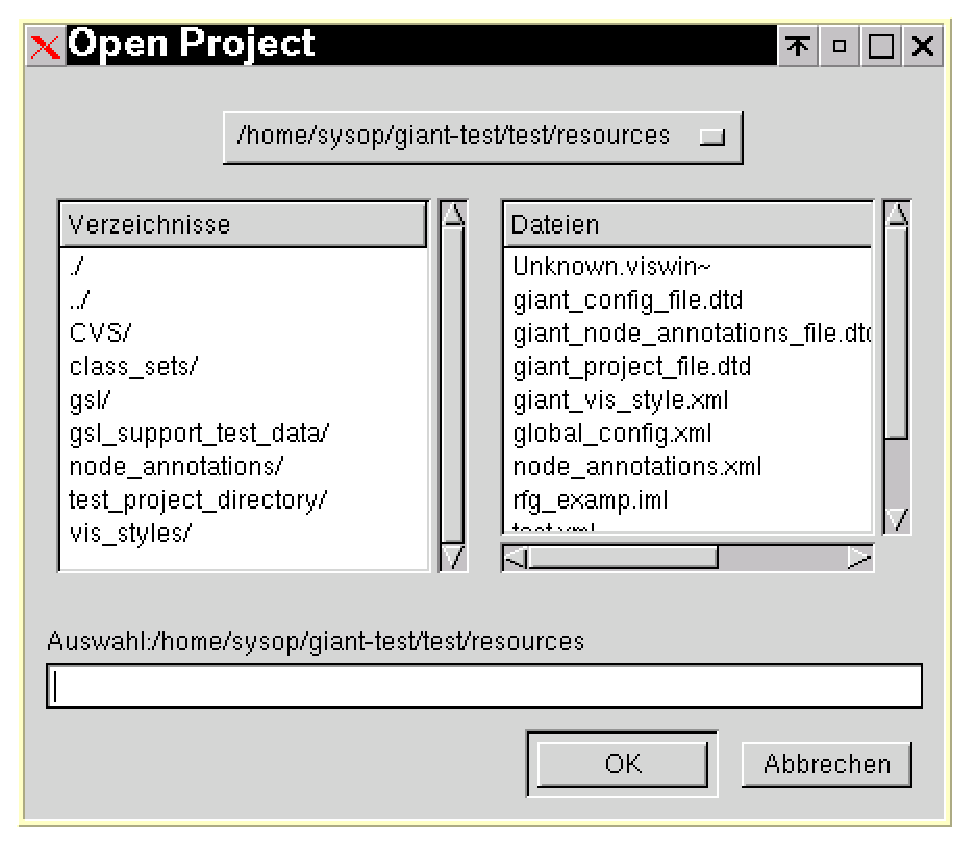
\includegraphics{gui/filechooser_dialog}
       \caption{Filechooser-Window}
       \label{Filechooser-Window-Pic}
    \end{figure}

Die Auswahl von Dateien (Laden/Speichern) passiert bei GIANT mittels
des Standard-Filechooser-Dialogs (siehe Abbildung \ref{Filechooser-Window-Pic}). 
Dieser Dialog ist Bestandteil der Widget-Bibliothek von GTK.


% ******** Gibt es den Fadenkreuz-Cursor?
\section{Fadenkreuz-Cursor}
\label{Fadenkreuzcursor}
        Der Cursor verwandelt sich nach Auswahl bestimmter
        Funktionen (siehe z.B. Funktion \ref{Platz Schaffen-Dialog}) in ein Fadenkreuz.
        Durch Linksklick auf einen Fenster-Knoten oder eine 
        Fenster-Kante in einem Anzeigefenster  
        wird diese(r) f�r die jeweilige Funktion ausgew�hlt. 
        Der Fadenkreuz-Cursor wird auch zur Vorgabe von Positionen,
        an denen dann z.B. neue Fenster-Knoten eingef�gt werden,
        verwendet.
        Nach dem Linksklick  verwandelt
        sich der Fadenkreuz-Cursor wieder in den Standard-Cursor.
        Durch einen Rechtsklick bei aktivem Fadenkreuz-Cursor l�sst sich 
        die aktuelle Funktion abbrechen.




%%% Local Variables: 
%%% TeX-master: "spec"
%%% End: 



%===============================================================================
% 
% Anfragesprache
%
\chapter{GIANT Scripting Language}
\label {GIANT Scripting Language}

% 
% Moin Olly - Ich hab das Kapitel nach doc/handbuch/gsl.tex verschoben.
% Da kannst Du nun aaaaaaaaaaaaaaaaaalle Fragen beantworten! :-) -- Phil
%

% =============================================================================
%  $RCSfile: gsl.tex,v $ $Revision: 1.20 $
%  $Date: 2003-10-06 23:02:40 $
%  $Author: koppor $
%
%  Description: Spezifikation der GIANT Scripting Language
%
%  First Author: Steffen Keul
%
% =============================================================================


\documentclass[a4paper,titlepage,11pt,german,twoside]{scrbook}


\makeatletter

%koma uses \chapter*, but we want to use \chapter
%  changed srcbook.cls-commands
\renewcommand\idx@heading{%
  \twocolumn
  \chapter{\indexname}\@mkboth{\indexname}{\indexname}
}

%Nummerierung soll net so eng aneinanderhaengen
\renewcommand*\l@section{\@dottedtocline{1}{1.5em}{3em}}

\makeatother


\usepackage{../../styles/common}

\usepackage{../spec}

\usepackage{ebnf}

\usepackage{verbatim}
\usepackage{shortvrb}

\usepackage{makeidx}
\makeindex

% subsubsections nummerieren
\setcounter{secnumdepth}{3}

\newcommand\version{Version 1.5\xspace}
%\newcommand\version{\today\xspace}

% header
\fancyhead{}
\fancyhead[LE,RO]{\slshape \company}
\fancyhead[LO,RE]{\slshape \leftmark}
\fancyfoot[LE,RO]{\thepage{}}
\fancyfoot[LO,RE]{\version}

\begin{document}

% title page
\thispagestyle{empty}
\hfill
\parbox{5.5cm}
{Universit�t Stuttgart\\
Studienprojekt A -- IML Browser\\
\company}

\vspace{3cm}

\begin{center}
  \Huge
  \textsf{GIANT Scripting Language \\ Spezifikation}\\
  \vspace{.5cm}
  {\Large\version}\\
  \vspace{3cm}
  
\includegraphics[scale=.78]{../../logo}
\end{center}
\newpage

%\section*{Versionsgeschichte}

\begin{itemize}

\item Version 1.0 (08.04.2003)

  Diese Version wurde dem Kunden zur Pr�fung 
  im Kundenreview (14.04.2003 - 16.04.2003) vorgelegt.


\item Version 1.1 (22.04.2003)

  Die Korrekturen gem�� dem Kundenreview vom 14.04.2003 bis
  zum 16.04.2003 wurden eingearbeitet.\\
  Die Spezifikation der GSL (in Version 1.0 noch GQSL) wurde in 
  ein separates Dokument ausgelagert (siehe Kapitel 
  \ref {GIANT Scripting Language}).\\
  Diese Version der Spezifikation ging am 22.04.2003 
  zur Abnahme an den Kunden.

\end{itemize}

%%% Local Variables: 
%%% TeX-master: "spec"
%%% End: 


%==============================================================================
%
% Inhaltsverzeichnis
%
\setcounter{tocdepth}{1}
\tableofcontents

%%%%%%%%%%%%%%%%%%%%%%%%%%%%%%%%%%%%%%%%%%%%%%%%%%%%%%%%%%%%%%%%%%%%%%%%%%%%%%
%% Beginn des Texts
%%
%%%%%%%%%%%%%%%%%%%%%%%%%%%%%%%%%%%%%%%%%%%%%%%%%%%%%%%%%%%%%%%%%%%%%%%%%%%%%%
\chapter{GIANT Scripting Language}


\MakeShortVerb{\�}


%%%% Non-terminals

%%%% Tokens
\token{\tokbegincomment}{//}
\token{\tokbeginsequence}{[}
\token{\tokclosebracket}{)}
\token{\tokcurlyclose}{\}}
\token{\tokcurlyopen}{\{}
\token{\tokcomma}{,}
\token{\tokdot}{.}
\token{\tokendsequence}{]}
\token{\tokopenbracket}{(}
\token{\toknull}{null}
\token{\tokfalse}{false}
\token{\tokplus}{+}
\token{\tokselection}{selection}
\token{\toksemicolon}{;}
\token{\toksubgraph}{subgraph}
\token{\toktick}{'}
\token{\toktrue}{true}
\token{\tokquote}{''}
\token{\tokunderscore}{\_}

\nonterminal{\nidentifier}{identifier}
\nonterminal{\nchar}{char}
\nonterminal{\ndigit}{digit}
\nonterminal{\nliteral}{literal}
\nonterminal{\nbooleanliteral}{boolean\_literal}
\nonterminal{\nintliteral}{int\_literal}
\nonterminal{\nstringliteral}{string\_literal}
\nonterminal{\nstringchar}{direct\_char}
\nonterminal{\neverychar}{every\_char}
\nonterminal{\nnullliteral}{null\_literal}
\nonterminal{\nexpression}{expression}
\nonterminal{\ninspection}{inspection}
\nonterminal{\nvisiblevar}{visible\_var}
\nonterminal{\nglobalvar}{global\_var}
\nonterminal{\nsubgraph}{subgraph}
\nonterminal{\nselection}{selection}
\nonterminal{\nreference}{reference}
\nonterminal{\nvisibleref}{visible\_ref}
\nonterminal{\nvarcreation}{var\_creation}
\nonterminal{\nglobalref}{global\_ref}
\nonterminal{\nscriptdecl}{script\_decl}
\nonterminal{\nlist}{list}
\nonterminal{\nsequence}{sequence}
\nonterminal{\nscriptactivation}{script\_activation}

\newcommand{\bottomenv}{\ensuremath{First}\xspace}
\newcommand{\newenv}{\ensuremath{A_{neu}}\xspace}
\newcommand{\oldenv}{\ensuremath{A_{alt}}\xspace}
\newcommand{\startenv}{\ensuremath{A_{start}}\xspace}



In diesem Dokument wird die GIANT Scripting Language (GSL) sowie der
Interpreter zur Ausf�hrung von GSL Scripts spezifiziert.
GSL ist eine Skriptsprache f�r das Software-System GIANT. Mit Hilfe von
GSL k�nnen Anfragen an die IML-Bibliothek gestellt werden und auf den
Resultaten Aktionen ausgef�hrt werden.

Hier wird zun�chst die Struktur von IML-Graphen aus der Sicht
von GIANT beschrieben und danach die Syntax und Sematik von GSL definiert.
Schlie�lich folgt die vollst�ndige Beschreibung der angebotenen
Sprachumgebung.

\section{IML-Graphen}

Der Kunde stellt die Reflektion zur Verf�gung. GIANT verwendet diese
Bibliothek, um auf IML-Graph Dateien zuzugreifen.

\subsection{IML-Datenbasis}
\index{IML-Graph Datei!Inhalt}

In jeder IML-Graph Datei sind IML-Daten enthalten. Diese
bestehen aus
\begin{enumerate}
\item IML-Knoten
\item Attributen von IML-Knoten
\item nichts sonst.
\end{enumerate}

Es gibt in jeder IML-Graph Datei genau einen besonderen IML-Knoten,
der Wurzelknoten genannt wird.

\subsubsection{Attribute von IML-Knoten}

Jeder IML-Knoten hat einen Typ. F�r jeden Typ von IML-Knoten existiert ein
String, der den Typ eindeutig identifiziert.

Jeder IML-Knoten verf�gt �ber eine endliche Folge von Attributen.
Diese Folge definiert eine endliche Anzahl einzelner Attribute,
die der IML-Knoten besitzt, sowie eine Reihenfolge dieser Attribute.
Weder die Folge von Attributen noch die in der Folge enthaltenen
Attribute eines IML-Knoten k�nnen sich w�hrend der Laufzeit von
GIANT ver�ndern.

Jedes Attribut besitzt einen Attribut-Namen. Kein IML-Knoten besitzt
zwei verschiedene Attribute, die einen gleichen Namen besitzen.

Einige Attribute sind Verweise. Sie verweisen auf h�chstens einen
IML-Knoten. Es werden unterschieden:
\begin{description}
\item[Verweise] Verweise, die auf genau einen IML-Knoten verweisen.
\item[Nullverweise] Verweise, die auf einen besonderen Wert verweisen,
           der kein IML-Knoten ist. Ein Nullverweis ist kein Verweis.
\end{description}

Jedes Attribut eines IML-Knoten geh�rt genau einer der folgenden Klassen an:
\begin{description}
\item[Einfache Attribute]: Haben einen bestimmten Wert.
           M�gliche Typen dieses Werts sind:
           \begin{enumerate}
           \item Source Location
                 \begin{enumerate}
                 \item Zeilennummer (Natural)
                 \item Spaltennummer (Natural)
                 \item Filename (String)
                 \item Pfadname (String)
                 \end{enumerate}
           \item Boolean
           \item Natural
           \item String
           \item Folge von Strings
           \end{enumerate}
\item[Verweis-Attribut] Ein Verweis
\item[Nullverweis-Attribut] Ein Nullverweis. Ein Nullverweis-Attribut ist
kein Verweis-Attribut.
\item[Verweisfolgen-Attribut] Eine endliche Folge von Verweisen
\item[Verweismengen-Attribut] Eine endliche Menge von Verweisen
\end{description}



\subsection{IML-Graphen}
\hyphenation{kanten-annotierter}

Die IML-Daten jeder IML-Graph Datei definieren einen zugeh�rigen IML-Graph.
Sprechweise: Die IML-Daten liegen dem IML-Graph zugrunde.
Ein IML-Graph ist ein gerichteter knoten- und kantenannotierter Graph mit
Schlingen und Mehrfachkanten. Er ist definiert durch die folgende
Vorschrift:

\begin{enumerate}
\item
Ein IML-Graph besitzt als Knotenmenge die Menge aller IML-Knoten der
zugrunde liegenden IML-Daten. Der IML-Graph besitzt keine
weiteren Knoten.
\item
Annotationen eines IML-Knoten sind alle Attribute des IML-Knoten.
\item
\label{edge_spec}
Eine Kante im IML-Graph hei�t IML-Kante. Eine IML-Kante $e$ von einem
IML-Knoten $v$ zu einem IML-Knoten $w$ des selben IML-Graph existiert
genau dann, wenn eine der folgenden Bedingungen erf�llt ist:
   \begin{enumerate}
   \item $v$ besitzt ein Verweis-Attribut, das auf $w$ verweist.
         \begin{enumerate}
         \item Dann besitzt $e$ als Annotation den Attribut-Namen $s$ des
         Verweis-Attributs.
         \item Das Paar $(type (v), s)$ hei�t Typ der IML-Kante $e$
         \end{enumerate}
   \item $v$ besitzt ein Verweisfolgen-Attribut $f$. Ein Verweis
         aus $f$ verweist auf $w$.
         \begin{enumerate}
         \item dann besitzt $e$ als Annotation den Attribut-Namen $s$ von
         $f$ sowie
         die Nummer innerhalb der Folge $f$ des Verweises auf $w$.
         \item Das Paar $(type (v), s)$ hei�t Typ der IML-Kante $e$.
         \end{enumerate}
   \item $v$ besitzt ein Verweismengen-Attribut $m$. Ein Verweis
         aus $m$ verweist auf $w$.
         \begin{enumerate}
         \item dann besitzt $e$ als Annotation den Attribut-Namen $s$ von $m$.
         \item Das Paar $(type (v), s)$ hei�t Typ der IML-Kante $e$.
         \end{enumerate}
   \end{enumerate}
\item Falls eine IML-Kante $e$ existiert, so hat $e$ keine Annotationen,
au�er den in Punkt \ref{edge_spec} genannten.
\end{enumerate}



\section{GSL Interpreter}

Ein GSL Interpreter ist ein System, das GSL Ausdr�cke auswertet, gem��
der Sprachdefinition in Kapitel \ref{gsl_spec}. Jeder GSL
Interpreter muss die vordefinierte Sprachumgebung nach Kapitel
\ref{predef_env} unterst�tzen.

\subsection{Start einer Auswertung}
\label{interpreter_start}

Beim Start des GSL Interpreters erzeugt dieser zun�chst die erste
Aktivierungsumgebung \bottomenv. Danach ist der GSL Interpreter bereit
und ihm kann ein beliebiger GSL Ausdruck
zur Auswertung �bergeben werden. In GIANT kann dies geschehen, indem der
Ausdruck als Kommandozeilenparameter angegeben wird oder indem ein Ausdruck
in das daf�r vorgesehene Anzeigefenster eingegeben wird.

Dieser Ausdruck kann gespeicherte GSL Scripts aufrufen und mit GIANT
kommunizieren.

\subsection{Kontext des Interpreters}

Der GSL Interpreter kann im Kontext eines GIANT-Anzeigefensters ausgef�hrt
werden. Ist dies der Fall, so k�nnen die ausgewerteten GSL Ausdr�cke
Aktionen in diesem Anzeigefenster durchf�hren.

Wird der GSL Interpreter nicht im Kontext eines Anzeigefensters ausgef�hrt,
so k�nnen die GSL Ausdr�cke keine Aktion in einem Anzeigefenster
ausl�sen.

Ein GSL Script kann den GSL Interpreter anweisen in den Kontext eines
bestimmten Anzeigefensters zu wechseln.

\subsection{Verhalten im Fehlerfall}

\subsubsection{Syntaxfehler}
\label{syntax_error}

Der GSL Interpreter muss einen Ausdruck zur�ckweisen, falls eine
Forderung der Sprachdefinition durch diesen Ausdruck verletzt
wird. In diesem Fall muss der Interpreter dem Benutzer eine Fehlermeldung
anzeigen.
Andernfalls startet der GSL Interpreter die Auswertung des GSL Ausdrucks.

\subsubsection{Laufzeitfehler}
\label{run_time_error}

Der GSL Interpreter muss die Ausf�hrung sofort
stoppen, sobald ein Laufzeitfehler auftritt. Dies kann nur dann
geschehen und muss jedes Mal geschehen,
wenn die Semantikdefinition es vorschreibt. Der GSL Interpreter
darf die Ausf�hrung bereits nach einem fr�heren Ausf�hrungsschritt abbrechen,
wenn sichergestellt ist, dass nach einem sp�teren Ausf�hrungsschritt
ein Laufzeitfehler auftreten wird.
Der GSL Interpreter zeigt dem Benutzer eine Fehlermeldung an.

Der GSL Interpreter muss nach einem Fehler entweder alle seit Beginn
der Ausf�hrung bereits ausgef�hrten Aktionen r�ckg�ngig machen, oder er
muss dem Benutzer anzeigen, welche Aktionen bereits ausgef�hrt wurden,
bevor der Fehler passierte.

\section{Konzepte}

Der Entwurf von GSL legt das gr��te Gewicht auf eine einfache Erweiterbarkeit
der Ausdrucksm�chtigkeit der Sprache. Durch Hinzuf�gen von zus�tzlichen
vordefinierten Scripts k�nnen der Sprache neue F�higkeiten hinzugef�gt werden
ohne dabei �nderungen an der Syntax vornehmen zu m�ssen. Diesem wichtigsten
Ziel wurden Aspekte wie eine intuitiv erfassbare Syntax untergeordnet.

\subsection{Werte und Typen}
\label{types}

\newcommand\typename[2]{\newcommand{#1}{{\sf #2}\xspace}}
\typename{\tnodeid}{Node\_Id}
\typename{\tedgeid}{Edge\_Id}
\typename{\tnodeset}{Node\_Set}
\typename{\tedgeset}{Edge\_Set}
\typename{\tobjectset}{Object\_Set}
\typename{\tsloc}{Source\_Location}
\typename{\tstring}{String}
\typename{\tboolean}{Boolean}
\typename{\tnatural}{Natural}
\typename{\tlist}{List}
\typename{\tvarreference}{Var\_Reference}
\typename{\tscriptreference}{Script\_Reference}

\subsubsection{Vordefinierte Typen}

GSL verarbeitet Werte verschiedener Typen. Werte k�nnen das Ergebnis der
Auswertung von Ausdr�cken sein. Werte k�nnen in Objekten gespeichert werden.

Nachfolgend wird eine Liste aller
Typen sowie der Werte angegeben, die ein Ausdruck des entsprechenden Typs
annehmen kann:
\begin{description}
\item[\tnodeid] Verweis auf einen einzelnen Knoten.
\item[\tedgeid] Verweis auf eine einzelne Kante.
\item[\tnodeset] Endliche Menge von Werten des Typs \tnodeid.
\item[\tedgeset] Endliche Menge von Werten des Typs \tedgeid.
\item[\tstring] Endliche Folge von Zeichen.
\item[\tboolean] Der Wahrheitswerte \tokfalse und \toktrue
\item[\tnatural] Nat�rliche Zahl, innerhalb eines bestimmten Bereichs, der
von der Reflektion vorgegeben wird.
\item[\tlist] Endliche Folge von Werten. Jeder dieser Werte ist ein Wert
eines beliebigen Typs aus dieser Aufz�hlung oder \toknull.
\item[\tvarreference] Zugriffspfad auf ein Objekt.
\item[\tscriptreference] Aktivierungsinformation f�r ein bestimmtes Script.
\end{description}

Zus�tzlich gibt es noch einen besonderen Typ, der keinen Namen besitzt.
Dieser anonyme Typ umfasst genau einen Wert, n�mlich den Wert \toknull.

Alle diese Typen decken alle Typen der IML-Reflection ab. Falls
zur IML-Reflection neue Typen hinzugef�gt werden, so werden diese
ebenfalls in der GSL eingef�hrt.

\subsubsection{Zusammengesetzte Typen}

Werte zusammengesetzter Typen sind zusammengesetzt aus mehreren Werten
der vordefinierten Typen. In dieser Spezifikation wird im Folgenden nicht
mehr zwischen vordefinierten und zusammengesetzten Typen unterschieden.

\begin{description}
\item[\tobjectset] Wert des vordefinierten Typs \tlist mit genau zwei
Eintr�gen $N$ und $E$. Dabei muss $N$ ein Wert des Typs \tnodeset und $E$
ein Wert des Typs \tedgeset sein.
\item[\tsloc] Wert des vordefinierten Typs \tlist mit genau vier Eintr�gen
$L$, $S$, $F$, $P$. Dabei muss gelten:
 \begin{enumerate}
 \item $L$ ist vom Typ \tnatural (\gq{Zeilennummer}).
 \item $S$ ist vom Typ \tnatural (\gq{Spaltennummer}).
 \item $F$ ist vom Typ \tstring (\gq{Filename}).
 \item $P$ ist vom Typ \tstring (\gq{Pfadname}).
 \end{enumerate}
\end{description}

\subsection{Ausdr�cke}

Die Ausf�hrung von GSL geschieht ausschlie�lich durch das Auswerten von
Ausdr�cken. Die Auswertung eines Ausdrucks hat als Ergebnis stets genau
einen bestimmten Wert und kann Nebeneffekte haben. Nebeneffekte sind
Ver�nderungen an den Werten von Objekten oder die Durchf�hrung von Aktionen.

Der Typ eines Ergebnisses steht im Allgemeinen erst fest, nachdem ein Ausdruck
ausgewertet wurde. Die Auswertung eines Ausdrucks kann fehlschlagen, falls
ein Laufzeitfehler auftritt. In diesem Fall stoppt die Auswertung sofort.

\subsection{Variablen und Objekte}
\label{variables}

Um w�hrend der Auswertung von Ausdr�cken bestimmte Werte zur sp�teren
Wiederverwendung zu speichern werden \emph{Objekte} verwendet. Der Zugriff
auf ein Objekt erfolgt durch eine Variable oder einen Zugriffspfad.

In \emph{Aktivierungsumgebungen} werden Variablen an Objekte gebunden.

\label{variable_inspection}
Variablen k�nnen \emph{inspiziert} werden. Das Ergebnis einer
Variableninspektion ist der Wert des Objekts, an das die Variable gebunden
ist.

\label{variable_reference}
Eine \emph{Referenz} einer Variable kann genommen werden.
Diese Referenz ist ein
Zugriffspfad auf das Objekt an das die Variable gebunden ist. Der
Zugriffspfad wird ben�tigt, um den Wert des Objekts zu ver�ndern.

Eine Variable kann entweder sichtbar oder unsichtbar sein. Siehe hierzu
Kapitel \ref{visibility}.

Jedes Objekt kann einen Wert $w_1$ jedes beliebigen Typs $t_1$ aus
\ref{types} annehmen. Durch eine weitere Zuweisung an das Objekt kann
das Objekt einen anderen Wert $w_2$ des Typs $t_2$ annehmen. Dabei d�rfen
die beiden Werte aus verschiedenen Typen sein (dh.\ $t_1 \neq t_2$ ist
zul�ssig).

\subsection{Aktivierungsumgebungen}

\subsubsection{Standard-Aktivierungsumgebung}

\label{bottom_env}
Eine Aktivierungsumgebung bindet Variablen an Objekte. Beim Start des GSL
Interpreters existiert eine erste Aktivierungsumgebung \bottomenv.

In \bottomenv existiert f�r jeden zul�ssigen Namen �<Name>� eines
IML-Teilgraphen in GIANT eine Variable \gq{\toksubgraph\tokdot�<Name>�}.
(Es gibt also aufz�hlbar unendlich viele solche Variablen.)
Jede dieser Variablen ist an den IML-Teilgraphen mit dem entsprechenden
Namen �<Name>� gebunden, sofern dieser IML-Teilgraph existiert.
Existiert der IML-Teilgraph nicht, so ist die Variable an ein besonderes
Objekt gebunden, das den Wert \toknull hat.

Falls der GSL Interpreter im Kontext eines Anzeigefensters $W$ ausgef�hrt wird,
dann existiert in \bottomenv f�r jeden zul�ssigen Namen �<Name>� einer
Selektion im Fenster $W$ eine Variable \gq{\tokselection\tokdot�<Name>�}.
(Es gibt also aufz�hlbar unendlich viele solche Variablen.)
Jede dieser Variablen ist an die Selektion mit dem entsprechenden
Namen �<Name>� gebunden, sofern diese Selektion existiert.
Existiert die Selektion nicht, so ist die Variable an ein besonderes
Objekt gebunden, das den Wert \toknull hat. Wird der GSL Interpreter nicht
im Kontext einen Anzeigefensters ausgef�hrt, so existiert keine dieser
Variablen.

Die erste Aktivierungsumgebung \bottomenv ist anfangs \emph{aktuell}.

\subsubsection{Vererbung von Aktivierungsumgebungen}
\label{current_env}

Wann immer der GSL Interpreter die Auswertung eines benutzerdefinierten
GSL Ausdrucks startet (siehe \ref{interpreter_start}), wird eine neue
Aktivierungsumgebung \startenv erzeugt. \startenv \emph{beerbt} dabei
\bottomenv. \startenv wird aktuell bevor die Auswertung des benutzerdefinierten
Ausdrucks beginnt. Nachdem die Auswertung abgeschlossen ist, wird \startenv
zerst�rt und \bottomenv wird wieder aktuell.

Falls w�hrend der Auswertung eines Ausdrucks die Aktivierung eines Scripts
erfolgt, so wird eine neue Aktivierungsumgebung f�r die Auswertung
dieses Scripts erzeugt. Diese neue Aktivierungsumgebung \newenv beerbt eine
bestimmte Aktivierungsumgebung \oldenv, die durch die Aktivierungsinformation
bestimmt wird (siehe \ref{script_activation}). \newenv wird aktuell.
Nachdem die Auswertung des Script beendet ist wird \newenv zerst�rt und \oldenv
wird wieder aktuell.

W�hrend ein Script ausgewertet wird, k�nnen weitere Scripts aktiviert werden.
Deshalb k�nnen mehrere Aktivierungsumgebungen gleichzeitig existieren. Auf
diesen Aktivierungsumgebungen existiert eine Vererbungsbeziehung die durch
eine partielle Ordnung beschrieben $\le$ werden kann:
\begin{enumerate}
\item F�r zwei Aktivierungsumgebungen $A_1, A_2$ gilt: $($ falls $A_2$ beerbt
$A_1 ) \Rightarrow A_1 \le A_2$
\item F�r jede Aktivierungsumgebung $A$ gilt: $A \le A$
\item F�r zwei Aktivierungsumgebung $A_1, A_2$ gilt:
$A_1 \le A_2 \wedge A_2 \le A_1 \Rightarrow A_1 = A_2$
\item F�r drei Aktivierungsumgebungen $A_1, A_2, A_3$ gilt:
$A_1 \le A_2 \wedge A_2 \le A_3 \Rightarrow A_1 \le A_3$
\end{enumerate}

\textbf{Anmerkung} Weil nach Start des GSL Interpreters eine erste
Aktivierungsumgebung \bottomenv erzeugt wird, aufgrund der beschriebenen
Vererbung und aufgrund der Transitivit�t
von $\le$ gilt f�r jede Aktivierungsumgebung $A$:
$\bottomenv \le A$.

\subsubsection{Sichtbarkeit}
\label{visibility}

Annahme: Die Aktivierungsumgebung \newenv beerbt die Aktivierungsumgebung
\oldenv. Dann bindet \newenv mindestens alle Variablen, die
auch \oldenv bindet. In \newenv k�nnen zus�tzlich
\begin{enumerate}
\item weitere Variablen gebunden werden, die in \oldenv nicht gebunden
sind.
\item Variablen, die in \oldenv gebunden sind, an andere Objekte
gebunden werden (�berladen).
\end{enumerate}

Eine Variable $v$ hei�t \emph{lokal} in \newenv, falls sie eine der
folgenden Bedingungen erf�llt:
\begin{enumerate}
\item Es existiert keine Aktivierungsumgebung \oldenv, die von \newenv
beerbt wird oder
\item \newenv beerbt \oldenv. $v$ ist in \oldenv an ein Objekt $o_1$
gebunden ist und $v$ ist in \newenv an ein Objekt $o_2$ mit $o_1 \neq o_2$
gebunden oder
\item \newenv beerbt \oldenv. $v$ ist in \oldenv nicht gebunden, und
$v$ ist in \newenv gebunden an irgend ein Objekt.
\end{enumerate}

Jede Variable, die in \newenv an irgend ein Objekt gebunden ist, hei�t
\emph{sichtbar} in \newenv.

Jede Variable, die in \newenv sichtbar ist, aber nicht lokal in \newenv ist,
hei�t \emph{global} in \newenv.

\textbf{Anmerkung} In einer Aktivierungsumgebung $A_1$ sind alle Variablen
sichtbar, die in irgend einer Aktivierungsumgebung $A_2$ mit $A_2 \le A_1$
sichtbar sind.

\paragraph{Beispiel}

\verbatiminput{visibility.gsl}

\subsection{Aktivierung von Scripts}

Ein Script ist ein Paar aus
\begin{description}
\item[Parameterliste] einer (m�glicherweise leeren) Liste von Ausdr�cken,
deren Ergebnis Zugriffspfade auf Objekte sein m�ssen.
\item[Rumpf] einem Ausdruck.
\end{description}

\paragraph{Beispiel einer Script-Deklaration}

\verbatiminput{scriptdecl.gsl}

\subsubsection{Ablauf der Aktivierung}
\label{activation_process}

Ein Script $S$ kann \emph{aktiviert} werden. Wenn $S$ aktiviert wird, dann
wird eine neue Aktivierungsumgebung \newenv erzeugt. Es werden die Argumente
des Aufrufs an die Parameter von $S$ �bergeben. Der Rumpf von $S$ wird
ausgewertet. Das Ergebnis der Auswertung von $S$ ist das Ergebnis der
Auswertung des Rumpfs von $S$. F�r die genaue Beschreibung siehe
\ref{script_activation}.

\subsubsection{Vorraussetzung}
\label{activation_preconds}

Ein Script $S$ wird aktiviert durch Auswertung eines Ausdrucks, der als
Ergebnis einen
Wert des Typs \tscriptreference hat. Dieser Wert wird als
Aktivierungsinformation bezeichet.

Die Aktivierungsinformation bestimmt
\begin{enumerate}
\item Welches Script ausgef�hrt wird (Quelltext-Position von $S$ oder eine
gleichwertige Darstellung).
\item Welche Aktivierungsumgebung beerbt wird, wenn die Aktivierung
stattfindet. \label{allowed_environments}
\end{enumerate}

Vor der Aktivierung des Scripts $S$ wird eine neue Aktivierungsumgebung
\newenv erzeugt und danach aktuell.
Das zu aktivierende Skript $S$ kann eine in \newenv globale Variable
$v$ inspizieren, oder die Referenz von $v$ nehmen.
Es soll sichergestellt werden, dass die neue Aktivierungsumgebung \newenv nur
solche Aktivierungsumgebungen \oldenv beerben kann, so dass die Variable $v$
in \oldenv genau die Bedeutung hat, die der Autor von $S$ erwartet.
Dies stellt Punkt \ref{allowed_environments} der vorangehenden Aufz�hlung
sicher. \oldenv ist \emph{nicht} zwangsl�ufig die vor der Aktivierung von
$S$ aktuelle Aktivierungsumgebung. \oldenv ist diejenige Aktivierungsumgebung,
die zum Zeitpunkt der Auswertung der Script-Deklaration von $S$
(siehe \ref{script_decl}) aktuell war.

\paragraph{Beispiel zur Scriptaktivierung}

\verbatiminput{activation.gsl}

\subsubsection{Parameter�bergabe}
\label{parameter_passing}

In dem Ausdruck dessen Auswertung die Aktivierung eines Scripts veranlasst
wird eine Liste von Argumenten $L_e = (e_1, ..., e_n)$ angegeben mit
$n \in {0, 1, 2, ...}$ und $\forall 1 \le i \le n: (e_i$ ist ein Ausdruck$)$.
Bevor die Aktivierung beginnt, wird
$L_e$ ausgewertet und hat als Ergebnis den Wert $L_a = (a_1, ..., a_n)$.

Nachdem die Aktivierung begonnen hat, wird
die Parameterliste ausgewertet (siehe Abschnitt \ref{script_activation}).
Das Ergebnis dieser Auswertung muss ein Wert $L_p$ vom Typ
\tlist sein. Es muss gelten $L_p = (p_1, ..., p_n)$ mit
$\forall 1 \le i \le n: ( p_i$ ist ein Zugriffspfad auf ein Objekt$)$.
Andernfalls f�hrt die Auswertung zu einem Laufzeitfehler.

Dann wird f�r alle $i$ jedem Objekt, das durch den Zugriffspfad $p_i$ erreicht
wird, der Wert $a_i$ zugewiesen. In GSL formuliert wird der Ausdruck
�(set (�$p_1$�, �$a_1$�), ..., set (�$p_n$�, �$a_n$�))�
ausgewertet und sein Ergebnis verworfen (Hinweis: Dieser Ausdruck ist kein
korrekter GSL-Ausdruck, sondern dient nur der intuitiven Erl�uterung).

Danach ist die Parameter�bergabe abgeschlossen und der Rumpf des Scripts wird
ausgewertet.

\textbf{Richtlinie} F�r die Parameter $p_i$ sollte jeweils eine
neue lokale Variable erzeugt werden, z.B. durch \gq{�+name�}.

\paragraph{Beispiel zur Parameter�bergabe}

\verbatiminput{parameters.gsl}

%%%%%%%%%%%%%%%%%%%%%%%%%%%%%%%%%%%%%%%%%%%%%%%%%%%%%%%%%%%%%%%%%%%%%%%%%%%%%%
\section{Syntax und Semantik}
\label{gsl_spec}

\subsection{Notation}

Die Syntax von GSL wird als kontextfreie Grammatik beschrieben.
\begin{enumerate}
\item Nichtterminale werden in einer serifenlosen Schrift dargestellt
(z.B. \nidentifier).
\item Terminalsymbole werden fett gedruckt (z.B. \toknull).
\item Eine Regel wird geschrieben als 
\begin{EBNF}
\item[{\sl linke Seite}] {\sl rechte Seite}
\end{EBNF}
wobei auf der linken Seite genau ein Nichtterminal steht, das bei Anwendung
der Regel durch die rechte Seite ersetzt werden darf.
\item Alternativen werden angegeben als
{\sl erste M�glichkeit} | {\sl zweite M�glichkeit}
\item Die Klammern $\langle$ {\sl Inhalt} $\rangle$ werden verwendet um ihren
Inhalt zusammenzufassen.
\item Ein Teil kann gar nicht, einmal oder beliebig oft expandiert werden,
wenn er von einem * gefolgt wird.
\item Ein Teil ist optional, falls er von einem $?$ gefolgt wird.
\end{enumerate}

Die Beschreibung der Bedeutung einer Regel erfolgt in einer Aufz�hlung, die
unter der Regel steht. In der Beschreibung werden
die Nichtterminale aus der rechten Seite der Regel als Platzhalter
f�r ihre Ableitung (also den Terminalstring zu dem sie im Programmtext
erweitert sind) verwendet.

\subsection{Schl�sselw�rter und lexikalische Elemente}
\label{tokens}

\begin{tabular}{l l l l}
\tokopenbracket & \tokclosebracket & \tokcurlyopen  & \tokcurlyclose \\
\tokbeginsequence & \tokendsequence & \tokcomma & \tokdot \\
\toksemicolon & \toktick & \tokplus & \tokunderscore \\

\tokselection & \toksubgraph & \tokbegincomment & \tokquote \\
\tokfalse & \toktrue & \toknull & �\� \\
\end{tabular}

Es wird zwischen Gro�- und Kleinschreibung unterschieden.

%%%%%%%%%%%%%%%%%%%%%%%%%%%%%%%%%%%%%%%%
\subsection{Kommentare}

In GSL-Dateien k�nnen Kommentare eingegeben werden, die auf die Semantik
des Programms keinen Einfluss haben. Ein Kommentar beginnt mit \tokbegincomment
und endet am Ende der Zeile. Alle Zeichen dazwischen geh�ren zu dem Kommentar.

%%%%%%%%%%%%%%%%%%%%%%%%%%%%%%%%%%%%%%%%
\subsection{White Space}

Leerzeichen, Tabulatoren, Zeilenumbr�che und Kommentare werden als Trennzeichen
verwendet. Zwischen Schl�sselw�rtern, den in \ref{tokens} aufgef�hrten
Zeichen und \nidentifier d�rfen beliebig viele Trennzeichen geschrieben werden.

%%%%%%%%%%%%%%%%%%%%%%%%%%%%%%%%%%%%%%%%
\subsection{Identifier}

\begin{EBNF}
\item[\nidentifier] \nchar $\langle$ \nchar | \ndigit | \tokunderscore
 $\rangle$*
\end{EBNF}

Dabei steht \nchar f�r eines der Zeichen a-z, A-Z. \ndigit steht f�r eine
der Ziffern 0-9.

\begin{enumerate}
\item Der Text eines \nidentifier darf nicht gleich sein wie ein
GSL-Schl�sselwort (siehe \ref{tokens}).
\item Die Gro�- und Kleinschreibung eines \nidentifier wird
unterschieden (Beispiel: \gq{Name} $\neq$ \gq{name}).
\end{enumerate}

%%%%%%%%%%%%%%%%%%%%%%%%%%%%%%%%%%%%%%%%
\subsection{Literale}

\begin{EBNF}
\item[\nliteral] \nbooleanliteral | \nintliteral | \nstringliteral
                 | \nnullliteral
\end{EBNF}

\begin{enumerate}
\item Ein \nliteral hat einen bestimmten Typ, und als Ergebnis einen Wert
dieses Typs.
\item Typ und Wert eines \nliteral stehen bereits zum �bersetzungszeitpunkt
fest. (siehe entsprechendes Nichtterminal der rechten Seite).
\end{enumerate}

\subsubsection{Boolean-Literal}

\begin{EBNF}
\item[\nbooleanliteral] \tokfalse | \toktrue
\end{EBNF}

\begin{enumerate}
\item Ein \nbooleanliteral ist vom Typ \tboolean.
\item Der Wert ist \tokfalse, falls die rechte Seite \tokfalse gew�hlt wurde.
\item Der Wert ist \toktrue, falls die rechte Seite \toktrue gew�hlt wurde.
\end{enumerate}

\subsubsection{Integer-Literal}

\begin{EBNF}
\item[\nintliteral] \ndigit \ndigit{}*
\end{EBNF}

\begin{enumerate}
\item Ein \nintliteral ist vom Typ \tnatural.
\item Der Wert ist die Interpretation des Texts im Zehnersystem.
\end{enumerate}

\subsubsection{String-Literal}

\begin{EBNF}
\item[\nstringliteral] \tokquote $\langle$ �\�\tokquote |
                       �\\� | �\�n | �\�t |
                       \nstringchar $\rangle$*
                       \tokquote
\end{EBNF}

Dabei steht \nstringchar f�r jedes Zeichen des (implementationsabh�ngigen)
Zeichensatzes au�er den Zeichen �\� und \tokquote.

\begin{enumerate}
\item Ein \nstringliteral ist vom Typ \tstring.
\item Der Wert ist die ersetzte Folge von Zeichen zwischen den \tokquote.
\item Die Zeichenfolge �\�\tokquote wird dabei ersetzt durch
ein einfaches \tokquote.
\item �\\� wird ersetzt durch das Zeichen �\�.
\item �\�n wird ersetzt durch das Zeichen Zeilenumbruch.
\item �\�t wird ersetzt durch ein Tabulatorzeichen.
\end{enumerate}

\subsubsection{Null-Literal}

\begin{EBNF}
\item[\nnullliteral] \toknull
\end{EBNF}

\begin{enumerate}
\item Der Typ eines \nnullliteral ist der anonyme Typ. Dieser Typ hat keinen
Namen.
\item Der Wert ist \toknull.
\end{enumerate}

%%%%%%%%%%%%%%%%%%%%%%%%%%%%%%%%%%%%%%%%
\subsection{Ausdr�cke}

\begin{EBNF}
\item[\nexpression] \nliteral | \ninspection | \nreference | \nscriptdecl
                    | \nlist | \nsequence | \nscriptactivation
\end{EBNF}

\begin{enumerate}
\item \nexpression k�nnen zur Laufzeit \emph{ausgewertet} werden.
\item W�hrend der Auswertung kann ein Laufzeitfehler auftreten. In diesem
Fall stoppt die Auswertung (siehe \ref{run_time_error}).
\item Um eine \nexpression auszuwerten wird die entsprechende rechte Seite
ausgewertet. N�heres dazu ist der Beschreibung der rechten Seite zu entnehmen.
\item Die Auswertung einer \nexpression kann \emph{Seiteneffekte} haben.
Die Seiteneffekte h�ngen von der gew�hlten rechten Seite ab.
\item Die Auswertung einer \nexpression hat ein Ergebnis, falls kein
Laufzeitfehler aufgetreten ist. Das Ergebnis ist stets ein Wert eines
bestimmten Typs. Das Ergebnis ist identisch mit dem Ergebnis der
Auswertung der rechten Seite der gew�hlten Regel. Siehe Beschreibung der
rechten Seiten.
\end{enumerate}

%%%%%%%%%%%%%%%%%%%%
\subsubsection{Inspektion}

\begin{EBNF}
\item[\ninspection] \nvisiblevar | \nglobalvar
\end{EBNF}

\begin{enumerate}
\item Eine \ninspection inspiziert den Wert des Objekts, das an die
zu inspizierende Variable gebunden ist (siehe \ref{variable_inspection}).
\item Die verschiedenen rechten Seiten werden verwendet um zwischen
Variablen zu unterscheiden, die an GSL-Objekte gebunden sind, und
Variablen, die an IML-Teilgraphen oder Selektionen in GIANT gebunden sind.
\item Das Ergebnis der \ninspection ist identisch mit dem Ergebnis der
gew�hlten rechten Seite.
\end{enumerate}

\begin{EBNF}
\item[\nvisiblevar] \nidentifier
\end{EBNF}

\begin{enumerate}
\item Inspiziert das Objekt, das in der aktuellen Aktivierungsumgebung
an die sichtbare Variable mit Name
\nidentifier gebunden ist (siehe \ref{visibility}).
\item Falls keine sichtbare Variable dieses Namens existiert, dann ist
die Auswertung ein Laufzeitfehler. Andernfalls ist die Inspektion
erfolgreich.
\item Falls die Inspektion erfolgreich ist, so ist das Ergebnis der Wert
des Objekts an das die Variable gebunden ist.
\end{enumerate}

\label{global_inspection}
\begin{EBNF}
\item[\nglobalvar] $\langle$ \toksubgraph | \tokselection
                   $\rangle$ \tokdot \nidentifier
\end{EBNF}

\begin{enumerate}
\item Falls \toksubgraph angegeben ist:
  \begin{enumerate}
  \item Diese Inspektion ist eine Schnittstelle zu GIANT.
  \item Falls in GIANT ein IML-Teilgraph $T$ mit Namen \nidentifier existiert,
  dann ist das Ergebnis dieser Inspektion ein Wert $M$ vom zusammengesetzten
  Typ \tobjectset. $M$ enth�lt alle Graph-Knoten aus $T$ und alle
  Graph-Kanten aus $T$ und nichts sonst.
  \item Falls in GIANT $T$ nicht existiert, so ist das Ergebnis dieser
  Inspektion der Wert \toknull.
  \item Formal erfolgt eine Inspektion der Variable mit Namen
  \toksubgraph.\nidentifier. Diese Variable ist stets in der
  Aktivierungsumgebung \bottomenv gebunden und deshalb stets sichtbar.
  \end{enumerate}
\item Falls \tokselection angegeben ist:
  \begin{enumerate}
  \item Diese Inspektion ist eine Schnittstelle zu GIANT.
  \item Falls der GSL Interpreter im Kontext eines Anzeigefensters ausgef�hrt
  wird und in diesem Anzeigefenster eine Selektion $S$ mit Namen \nidentifier
  existiert, dann ist das Ergebnis dieser Inspektion ein Wert $M$ vom Typ
  \tobjectset.
  $M$ enth�lt alle Fenster-Knoten aus $S$ und alle Fenster-Kanten aus $S$
  und nichts sonst.
  \item Falls der GSL Interpreter im Kontext eines Anzeigefensters ausgef�hrt
  wird und in diesem Anzeigefenster keine Selektion mit Namen \nidentifier
  existiert, so ist das Ergebnis dieser Inspektion der Wert \toknull.
  \item Falls der GSL Interpreter nicht im Kontext eines Anzeigefensters
  ausgef�hrt wird, so ist die Auswertung dieser Inspektion ein Laufzeitfehler.
  \item Formal erfolgt eine Inspektion der Variable mit Namen
  \tokselection.\nidentifier. Diese Variable ist, falls der GSL Interpreter
  im Kontext eines Anzeigefensters ausgef�hrt wird, in der
  Aktivierungsumgebung \bottomenv gebunden und deshalb sichtbar. Falls
  der GSL Interpreter nicht im Kontext eines Anzeigefensters ausgef�hrt wird,
  so existiert die Variable nicht.
  \end{enumerate}
\end{enumerate}


%%%%%%%%%%%%%%%%%%%%
\subsubsection{Referenz}

\begin{EBNF}
\item[\nreference] \nvisibleref | \nvarcreation | \nglobalref
\end{EBNF}

\begin{enumerate}
\item Eine \nreference nimmt die Referenz einer Variable (siehe
\ref{variable_reference}). Die verschiedenen rechten Seiten werden
verwendet um Variablen zu unterscheiden, die in verschiedenen
Aktivierungsumgebungen gebunden sind.
\item Das Ergebnis der \nreference ist identisch mit dem Ergebnis der
gew�hlten rechten Seite.
\end{enumerate}

\begin{EBNF}
\item[\nvisibleref] \toktick \nidentifier
\end{EBNF}

\begin{enumerate}
\item Nimmt die Referenz der Variable mit Name
\nidentifier, die in der aktuellen Aktivierungsumgebung sichtbar ist
(siehe \ref{visibility}).
\item Falls in der aktuellen Aktivierungsumgebung keine sichtbare Variable
dieses Namens existiert, so f�hrt die
Auswertung zu einem Laufzeitfehler. Andernfalls ist die Auswertung
erfolgreich.
\item Falls die Auswertung erfolgreich ist, so ist das Ergebnis ein
Zugriffspfad auf das Objekt an das die Variable gebunden ist.
\end{enumerate}

\begin{EBNF}
\item[\nvarcreation] \tokplus \nidentifier
\end{EBNF}

\begin{enumerate}
\item Bindet in der aktuellen Aktivierungsumgebung (siehe \ref{current_env})
die Variable mit Namen \nidentifier an ein neues Objekt.
\item Falls in der aktuellen Aktivierungsumgebung bereits eine Variable
mit diesem Namen gebunden war, so f�hrt die Auswertung zu einem Laufzeitfehler.
Andernfalls ist die Auswertung erfolgreich.
\item Das neue Objekt hat den Wert \toknull.
\end{enumerate}

\begin{EBNF}
\item[\nglobalref] \toktick $\langle$ \toksubgraph | \tokselection $\rangle$
                              \tokdot \nidentifier
\end{EBNF}

\begin{enumerate}
\item Falls \toksubgraph angegeben ist:
  \begin{enumerate}
  \item Diese Zugriffspfadbestimmung ist eine Schnittstelle zu GIANT.
  \item Falls in GIANT kein IML-Teilgraph mit Name \nidentifier existiert, dann
  erzeugt GIANT diesen IML-Teilgraph. Er enth�lt keine Graph-Knoten und keine
  Graph-Kanten.
  \item Das Ergebnis ist ein Zugriffspfad auf den IML-Teilgraph mit Name
  \nidentifier.
  \end{enumerate}
\item Falls \tokselection angegeben ist:
  \begin{enumerate}
  \item Diese Zugriffspfadbestimmung ist eine Schnittstelle zu GIANT.
  \item Falls der GSL Interpreter nicht im Kontext eines Anzeigefensters
  ausgef�hrt wird, so f�hrt die Auswertung dieser Zugriffspfadbestimmung zu
  einem Laufzeitfehler. Andernfalls ist die Auswertung erfolgreich.
  \item Ist die Auswertung erfolgreich und existiert im Anzeigefenster keine
  Selektion mit Name \nidentifier, so erzeugt GIANT im Anzeigefenster diese
  Selektion. Sie enth�lt keine Fenster-Knoten und keine Fenster-Kanten.
  \item Ist die Auswertung erfolgreich, so ist das Ergebnis ein Zugriffspfad
  auf die Selektion mit Name \nidentifier in dem Anzeigefenster, in dessen
  Kontext der GSL Interpreter ausgef�hrt wird.
  \end{enumerate}
\end{enumerate}

%%%%%%%%%%%%%%%%%%%%
\subsubsection{Scriptdeklaration}
\label{script_decl}

\begin{EBNF}
\item[\nscriptdecl] \tokcurlyopen \nlist \nexpression \tokcurlyclose
\end{EBNF}

\begin{enumerate}
\item Eine \nscriptdecl deklariert ein neues Script $S$.
\item Ergebnis ist eine Aktivierungsinformation $I$ vom Typ
\tscriptreference f�r $S$.
\item Die zul�ssige Aktivierungsumgebung in $I$ ist die (zum Zeitpunkt der
Auswertung der \nscriptdecl) aktuelle Aktivierungsumgebung.
\item Die \nlist hei�t Parameterliste von $S$ (vgl. \ref{script_activation}).
\item Die \nexpression hei�t Rumpf von $S$ (vgl. \ref{script_activation}).
\end{enumerate}


%%%%%%%%%%%%%%%%%%%%
\subsubsection{Liste}

\begin{EBNF}
\item[\nlist] \tokopenbracket $\langle$ \nexpression
                $\langle$ \tokcomma \nexpression $\rangle$*
              $\rangle ?$ \tokclosebracket
\end{EBNF}

\begin{enumerate}
\item Eine \nlist kann ausgewertet werden und hat als Ergebnis einen Wert
vom Typ \tlist.
\item Zur Auswertung einer \nlist werden der Reihe nach von links nach rechts
alle \nexpression ausgewertet, falls �berhaupt welche angegeben sind.
\item Die Auswertung f�hrt zu einem Laufzeitfehler, falls die Auswertung einer
der \nexpression zu einem Laufzeitfehler f�hrt. Andernfalls ist die Auswertung
erfolgreich.
\item Falls die Auswertung erfolgreich ist, so ist das Ergebnis ein Wert
vom Typ \tlist, der die Ergebnisse aller \nexpression in
ihrer korrekten Reihenfolge enth�lt und sonst nichts.
\end{enumerate}

%%%%%%%%%%%%%%%%%%%%
\subsubsection{Sequenz}

\begin{EBNF}
\item[\nsequence] \tokbeginsequence $\langle$ \nexpression
                  \toksemicolon $\rangle$* \tokendsequence
\end{EBNF}

\begin{enumerate}
\item Eine \nsequence kann ausgewertet werden und hat ein Ergebnis.
\item Zur Auswertung einer \nsequence werden der Reihe nach von links nach
rechts alle \nexpression ausgewertet, falls �berhaupt welche angegeben sind.
\item Die Auswertung f�hrt zu einem Laufzeitfehler, falls die Auswertung einer
der \nexpression zu einem Laufzeitfehler f�hrt. Andernfalls ist die Auswertung
erfolgreich.
\item Falls die Auswertung erfolgreich ist, so ist das Ergebnis der Wert,
den die Auswertung der letzten (der am weitesten rechts stehenden)
\nexpression zum Ergebnis hatte. Falls die \nsequence keine \nexpression
enth�lt, so ist das Ergebnis \toknull.
\end{enumerate}

%%%%%%%%%%%%%%%%%%%%
\subsubsection{Scriptaktivierung}
\label{script_activation}

\begin{EBNF}
\item[\nscriptactivation] \nexpression \nlist
\end{EBNF}

\begin{enumerate}
\item Die \nexpression wird ausgewertet und hat als Ergebnis den Wert $I$.
\item Die \nlist wird ausgewertet.
\item $I$ muss vom Typ \tscriptreference sein.
Andernfalls f�hrt die Auswertung zu einem Laufzeitfehler. $I$ enth�lt einen
Zugriffspfad auf das Skript $S$.
\item Es wird eine neue Aktivierungsumgebung $A$ erzeugt. $A$ beerbt die
  in $I$ angegebene zul�ssige Aktivierungsumgebung
  (siehe \ref{script_decl}, \ref{activation_preconds}). \label{new_activation}
\item $A$ wird aktuelle Aktivierungsumgebung.
\item Die Parameterliste $P$ von $S$ wird ausgewertet.
\item $P$ muss genauso viele Werte enthalten wie \nlist, andernfalls ist
  dies ein Laufzeitfehler.
\item Falls einer der Werte
  in $P$ nicht vom Typ \tvarreference ist, so ist dies ein Laufzeitfehler.
\item Den \tvarreference in $P$ werden die Werte der Eintr�ge des Werts von
  \nlist zugewiesen
  (genaue Beschreibung siehe \ref{parameter_passing}).
\item Die \nexpression des durch $I$ referenzierten Scripts wird
ausgewertet und hat den Wert $R$ als Ergebnis.
$R$ darf ein Wert eines beliebigen Typs sein mit den Einschr�nkungen:
    \begin{enumerate}
    \item Ist $R$ vom Typ \tvarreference, dann ist $R$ ein Zugriffspfad
    auf ein Objekt, das in einer Aktivierungsumgebung \oldenv an eine
    Variable gebunden ist. Es muss gelten: \oldenv $< A$. Andernfalls liegt
    ein Laufzeitfehler vor.\\
    \textbf{Hinweis}
    Diese Einschr�nkung erzwingt, dass $R$ nicht ein Zugriffspfad auf
    ein Objekt sein kann, das an eine lokale Variable gebunden ist.
    \item Ist $R$ vom Typ \tscriptreference, dann ist $R$ eine
    Aktivierungsinformation. Die zul�ssige Aktivierungsumgebung dieser
    Aktivierungsinformation sei \oldenv. Es muss gelten: \oldenv $< A$. 
    Andernfalls liegt ein Laufzeitfehler vor.\\
    \textbf{Hinweis}
    Diese Einschr�nkung erzwingt, dass die Aktivierung von $R$ nicht
    die Existenz der (w�hrend der Auswertung von $S$) aktuellen
    Aktivierungsumgebung $A$ erfordert.
    \end{enumerate}
  \label{script_result}
\item $A$ wird zerst�rt. Alle Objekte, die von lokalen Variablen in $A$
  gebunden wurden d�rfen zerst�rt werden.
\item Die Aktivierungsumgebung, die zuvor (bis zum Schritt
   \ref{new_activation}) aktuell war, wird wieder aktuell.
\item Falls kein Laufzeitfehler aufgetreten ist, so ist das Ergebnis der
  Auswertung der Wert $R$ (siehe Punkt \ref{script_result}).
\end{enumerate}


%%%%%%%%%%%%%%%%%%%%%%%%%%%%%%%%%%%%%%%%%%%%%%%%%%%%%%%%%%%%%%%%%%%%%%%%%%%%%%
\raggedbottom
\section{Vordefinierte Sprachumgebung}
\label{predef_env}

\newenvironment{scriptdef}[1]
{%begin
  \begin{tabular}{|p{0.2\textwidth} p{0.2\textwidth} p{0.5\textwidth}|}
  \multicolumn{3}{l}{\textbf{{\large #1}}} \\
  \hline
}
{%end
  \hline
  \end{tabular}
}

\newcommand{\sparam}[3]{#1 & #2 & #3 \\}
\newcommand{\sresult}[2]{\hline \textbf{Ergebnis} & #1 & #2 \\}
\newcommand{\saction}[1]{\hline \multicolumn{3}{|p{0.9\textwidth}|}{#1} \\}


In diesem Kapitel werden Scripts beschrieben, die in GSL standardm��ig zur
Verf�gung stehen. Dabei wird folgende Form verwendet:

\begin{scriptdef}{Variablenname}
\sparam{Param\_Name}{Typ}{Beschreibung des Parameters. In der Spalte \gq{Typ}
werden alle m�glichen Typen aufgelistet, die zul�ssig sind. Falls ein Wert
eines anderen Typs �bergeben wird, so soll w�hrend der Auswertung des Scripts
ein Laufzeitfehler auftreten.}
\sparam{Second\_Name}{Typ}{Die Parameter werden in der Reihenfolge
aufgelistet, in der die entsprechenden Argumente angegeben werden m�ssen.}
\sresult{Typ}{Beschreibung des Ergebnis, in der Spalte \gq{Typ} wird eine
Zusicherung angegeben. Das Ergebnis muss ein Wert dieses Typs sein.}
\saction{Beschreibung der Funktion und des genauen Ablaufs des Scripts.
Der Variablenname ist der Name einer Variable, deren Inspektion eine
\tscriptreference auf das beschriebene Script zum Ergebnis hat.}
\end{scriptdef}


\subsection{Elementare Scripts}

Die hier beschriebenen Scripts realisieren elementare Funktionalit�t,
die der GSL
Interpreter direkt zur Verf�gung stellt. Der GSL Interpreter erzeugt die
Objekte, in denen die Aktivierungsinformation gespeichert ist vor
Beginn einer Auswertung. Der GSL
Interpreter erzeugt die hier genannten Variablen in der
Aktivierungsumgebung \bottomenv.

\subsubsection{Zuweisung}

%%% set
\begin{scriptdef}{set}
\sparam{lhs}{\tvarreference}{Zugriffspfad auf eine sichtbare Variable}
\sparam{rhs}{jeder Typ}{Zuzuweisender Wert eines beliebigen Typs. Es gibt
jedoch gewisse Einschr�nkungen (siehe Beschreibung)}
\sresult{}{\toknull}
\saction{Das Objekt, das durch lhs referenziert wird, �ndert seinen Wert
zu rhs. Falls rhs einen Wert eines der Typen 
  \begin{enumerate}
  \item \tscriptreference
  \item \tvarreference
  \end{enumerate}
hat, so muss f�r die Aktivierungsumgebungen gelten: $A_{rhs} \le A_{lhs}$,
andernfalls f�hrt die Auswertung zu einem Laufzeitfehler.

$A_{lhs}$ ist dabei die kleinste Aktivierungsumgebung, in der das durch lhs
referenzierte Objekt an eine Variable gebunden ist. $A_{rhs}$ ist die kleinste
Aktivierungsumgebung, in der das durch $A_{rhs}$ referenzierte Objekt
an eine Variable gebunden ist.

Durch diese Einschr�nkung wird sichergestellt, dass zu keinem Zeitpunkt ein
Wert eines der Typen \tscriptreference oder \tvarreference existiert,
der ein Objekt referenziert, das an keine Variable gebunden ist. Dieser Fall
k�nnte sonst eintreten nachdem eine Aktivierungsumgebung zerst�rt wurde.}
\end{scriptdef}

%%% deref
\begin{scriptdef}{deref}
\sparam{ref}{\tvarreference}{Zugriffspfad auf ein Objekt eines
  beliebigen Typs}
\sresult{Typ des Werts des referenzierten Objekts}{Wert des Objekts,
  das durch ref referenziert wird}
\saction{Liefert den Wert des Objekts, das durch eine Referenz gegeben
  wird. \gq{Dereferenziert} eine Referenz}
\end{scriptdef}

%%%%%%%%%%%%%%%%%%%%%%%%%%%%%%%%%
\subsubsection{Kontrollfluss}

%%% if
\begin{scriptdef}{if}
\sparam{condition}{\tboolean}{Ein Wert vom Typ
\tboolean}
\sparam{true\_branch}{jeder Typ}{Falls der Typ \tscriptreference ist, so muss
true\_branch die Aktivierunginformation f�r ein parameterloses Script sein,
dessen Ergebnis beliebigen Typs sein darf.}
\sparam{false\_branch}{jeder Typ}{Falls der Typ \tscriptreference ist, so muss
false\_branch die Aktivierunginformation f�r ein parameterloses Script sein,
dessen Ergebnis beliebigen Typs sein darf.}
\sresult{von Argumenten abh�ngig}{Siehe Beschreibung}
\saction{Falls condition erf�llt ist, so ist $c = $ true\_branch, andernfalls
$c = $ false\_branch.

Falls $c$ eine Aktivierungsinformation ist, so wird das referenzierte
Script ohne Argumente aktiviert. Ergebnis des Scripts if ist das Ergebnis
von $c$. Falls $c$ keine Aktivierungsinformation ist, so ist das Ergebnis
des Scripts if der Wert von $c$. \textbf{Vorsicht:} falls der Ausdruck
in true\_branch oder false\_branch Seiteneffekte hat, so ist ist die �bergabe
einer Aktivierungsinformation geraten. Andernfalls w�rde der Ausdruck
ausgewertet unabh�ngig davon, ob condition erf�llt ist, oder nicht.}
\end{scriptdef}

%%% loop
\begin{scriptdef}{loop}
\sparam{body}{\tscriptreference}{Aktivierungsinformation f�r parameterloses
Script mit Ergebnistyp \tboolean}
\sresult{}{\toknull}
\saction{Aktiviert body. Falls body das Ergebnis \toktrue hat, aktiviert
body so oft ein weiteres Mal, bis body das Ergebnis \tokfalse hat.}
\end{scriptdef}

%%% error
\begin{scriptdef}{error}
\sparam{message}{\tstring}{Fehlermeldung}
\sresult{}{}
\saction{L�st einen Laufzeitfehler geziehlt aus und veranlasst den GSL
Interpreter dem Benutzer die Fehlermeldung message anzuzeigen.}
\end{scriptdef}

%%% run
\begin{scriptdef}{run}
\sparam{file\_name}{\tstring}{Name einer Bibliothek. An diesen Namen wird
noch der Text \gq{.gsl} angeh�ngt}
\sresult{}{Ergebnis des ausgef�hrten Ausdrucks}
\saction{An den file\_name wird \gq{.gsl} angeh�ngt. Dann sucht der GSL
Interpreter die Standard Directories nach einem File mit dem Namen.
Dann f�hrt der GSL Interpreter den in diesem File enthaltenen GSL Ausdruck
in der aktuellen Aktivierungsumgebung aus. Mit Hilfe dieses Scripts k�nnen
Bibliotheken von benutzerdefinierten Scripts geladen werden. Eine Bibliothek
sollte eine \nsequence sein und in den \nexpression der \nsequence sollten
neue Variablen erzeugt werden, die die Aktivierungsinformation von den
Scripts der Bibliothek enthalten. \textbf{Hinweis} run ist das einzige
Script, zu dessen Aktivierung keine neue Aktivierungsumgebung erzeugt werden
muss. Der Ausdruck aus der geladenen Datei wird direkt in der aktuellen
Aktivierungsumgebung ausgef�hrt.}
\end{scriptdef}


%%%%%%%%%%%%%%%%%%%%%%%%%%%%%%%%%
\subsubsection{Rechenoperationen}

%%% add
\label{scriptdef_add}
\begin{scriptdef}{add}
\sparam{a}{\tnatural oder \tvarreference}{Entweder eine Zahl oder ein
Zugriffspfad auf ein Objekt, das einen Wert aus \tnodeset oder \tedgeset hat}
\sparam{b}{\tnatural bzw.\ \tnodeid bzw.\ \tedgeid bzw.\ \tnodeset
bzw.\ \tedgeset bzw.\ \tvarreference}{Abh�ngig von dem Typ
von a ebenfalls eine Zahl oder der entsprechende Elementtyp oder eine
entsprechende Menge oder ein Zugriffspfad auf ein Objekt des
entsprechenden Mengen-Typs}
\sresult{\tnatural bzw.\ der namenlose Typ}{Abh�ngig von den Argumenten
entweder die Summe der beiden Zahlen oder der Wert \toknull}
\saction{Es werden verschiedene Verwendungen unterschieden:
\begin{enumerate}
\item a ist vom Typ \tnatural und b ist vom Typ \tnatural. Dann hat
die Aktivierung dieses Script die Summe der beiden Zahlen als
Ergebnis. Es ist ein Laufzeitfehler, falls der
(implementationsabh�ngige) maximale Wertebereich �berschritten wird.
\item a ist vom Typ \tvarreference und hat als Wert einen Zugriffspfad auf
ein Objekt, dessen Wert $N$ vom Typ \tnodeset ist. Das Ergebnis der
Script-Aktivierung ist in diesem Fall stets \toknull.
  \begin{enumerate}
  \item Falls b vom Typ \tnodeid ist, dann wird der Wert $N$ um das
  Element b vergr��ert, falls b zuvor noch nicht in $N$ enthalten war, 
  andernfalls wird nichts getan.
  \item Falls b vom Typ \tnodeset ist, dann wird die Vereinigung von
  $N$ und b gebildet und dem Objekt, das durch a referenziert wird,
  zugewiesen.
  \item Falls b vom Typ \tvarreference ist, dann muss b ein
  Zugiffspfad auf ein Objekt sein, dessen Wert $N_r$ vom Typ \tnodeset
  ist. In diesem Fall wird die Vereinigung von $N$ und $N_r$ gebildet
  und dem Objekt, das durch a referenziert wird, zugewiesen.
  \item Falls keiner dieser F�lle zutrifft, so ist dies ein Laufzeitfehler.
  \end{enumerate}
\item a ist vom Typ \tvarreference und hat als Wert einen Zugriffspfad auf
ein Objekt, dessen Wert $E$ vom Typ \tedgeset ist. Das Ergebnis der
Script-Aktivierung ist in diesem Fall stets \toknull.
  \begin{enumerate}
  \item Falls b vom Typ \tedgeid ist, dann wird der Wert $E$ um das
  Element b vergr��ert, falls b zuvor noch nicht in $E$ enthalten war, 
  andernfalls wird nichts getan.
  \item Falls b vom Typ \tedgeset ist, dann wird die Vereinigung von
  $E$ und b gebildet und dem Objekt, das durch a referenziert wird,
  zugewiesen.
  \item Falls b vom Typ \tvarreference ist, dann muss b ein
  Zugiffspfad auf ein Objekt sein, dessen Wert $E_r$ vom Typ \tedgeset
  ist. In diesem Fall wird die Vereinigung von $E$ und $E_r$ gebildet
  und dem Objekt, das durch a referenziert wird, zugewiesen.
  \item Falls keiner dieser F�lle zutrifft, so ist dies ein Laufzeitfehler.
  \end{enumerate}
\end{enumerate}}
\end{scriptdef}

%%% sub
\label{scriptdef_sub}
\begin{scriptdef}{sub}
\sparam{a}{\tnatural oder \tvarreference}{Entweder eine Zahl oder ein
Zugriffspfad auf ein Objekt, das einen Wert aus \tnodeset oder \tedgeset hat}
\sparam{b}{\tnatural bzw.\ \tnodeid bzw.\ \tedgeid bzw.\ \tnodeset
bzw.\ \tedgeset bzw.\ \tvarreference}{Abh�ngig von dem Typ
von a ebenfalls eine Zahl oder der entsprechende Elementtyp oder der
entsprechende Mengentyp oder ein Zugriffspfad auf ein Objekt des
entsprechenden Mengentyps}
\sresult{\tnatural bzw.\ der namenlose Typ}{Abh�ngig von den Argumenten
entweder die Differenz der beiden Zahlen oder der Wert \toknull}
\saction{Es werden verschiedene Verwendungen unterschieden:
\begin{enumerate}
\item a ist vom Typ \tnatural und b ist vom Typ \tnatural. Dann hat
dieses Script die Differenz a $-$ b der beiden Zahlen als Ergebnis. Es ist ein
Laufzeitfehler, falls der (implementationsabh�ngige) maximale Wertebereich
�berschritten wird.
\item a ist vom Typ \tvarreference und hat als Wert einen Zugriffspfad auf
ein Objekt, dessen Wert $N$ vom Typ \tnodeset ist. Das Ergebnis der
Script-Aktivierung ist in diesem Fall stets \toknull.
  \begin{enumerate}
  \item Falls b vom Typ \tnodeid ist, dann wird $N$ um das Element b
  verkleinert, falls b zuvor in $N$ enthalten war, andernfalls wird
  nichts getan.
  \item Falls b vom Typ \tnodeset ist, dann wird die Differenz $N-$ b
  gebildet und dem Objekt zugewiesen, das durch a referenziert wird.
  \item Falls b vom Typ \tvarreference ist, dann muss b ein Objekt
  referenzieren, dessen Wert $N_r$ vom Typ \tnodeset ist. In diesem
  Fall wird die Differenz $N-N_r$ gebildet und dem Objekt, das durch
  a referenziert wird, zugewiesen.
  \item Falls keiner dieser F�lle zutrifft, so ist dies ein Laufzeitfehler.
  \end{enumerate}
\item a ist vom Typ \tvarreference und hat als Wert einen Zugriffspfad auf
ein Objekt, dessen Wert $E$ vom Typ \tedgeset ist. Das Ergebnis der
Script-Aktivierung ist in diesem Fall stets \toknull.
  \begin{enumerate}
  \item Falls b vom Typ \tedgeid ist, dann wird der Wert $E$ um das
  Element b verkleinert, falls b zuvor in $E$ enthalten war,
  andernfalls wird nichts getan.
  \item Falls b vom Typ \tedgeset ist, dann wird die Differenz $E-$ b
  gebildet und dem Objekt zugewiesen, das durch a referenziert wird.
  \item Falls b vom Typ \tvarreference ist, dann muss b ein Objekt
  referenzieren, dessen Wert $E_r$ vom Typ \tedgeset ist. In diesem
  Fall wird die Differenz $E-E_r$ gebildet und dem Objekt, das durch
  a referenziert wird, zugewiesen.
  \item Falls keiner dieser F�lle zutrifft, so ist dies ein Laufzeitfehler.
  \end{enumerate}
\end{enumerate}}
\end{scriptdef}

%%% cat
\begin{scriptdef}{cat}
\sparam{left}{\tstring}{Der linke String}
\sparam{right}{\tstring}{Der rechte String}
\sresult{\tstring}{Konkatenation von left und right}
\saction{Berechnet die Konkatenation zweier Strings.}
\end{scriptdef}

%%%%%%%%%%%%%%%%%%%%%%%%%%%%%%%%%
\subsubsection{Vergleiche}

%%% less
\begin{scriptdef}{less}
\sparam{a}{\tnatural, \tedgeid, \tnodeid, \tstring}{}
\sparam{b}{der selbe Typ wie a}{}
\sresult{\tboolean}{Ergebnis der Ungleichung a < b}
\saction{Berechet Enthaltensein des Paars (a, b) in einer irreflexiven
antisymmetrischen und transitiven bin�ren Relation. Die Relation ist auf den
verschiedenen Typen folgenderma�en definiert:
\begin{description}
\item[\tnatural] Wie in der Mathematik f�r < �blich.
\item[\tedgeid] Implementationsabh�ngig, hat keine besondere Semantik, kann
verwendet werden um eine konsistente Sortierung verschiedener Listen zu
erreichen.
\item[\tnodeid] Implementierungsabh�ngig, hat keine besondere Semantik, kann
verwendet werden um eine konsistente Sortierung verschiedener Listen zu
erreichen.
\item[\tstring] Imlementierungsabh�ngige lexikographische Ordnung.
\end{description}}
\end{scriptdef}

%%% equal
\begin{scriptdef}{equal}
\sparam{a}{\tnatural, \tedgeid, \tnodeid, \tstring}{}
\sparam{b}{der selbe Typ wie a}{}
\sresult{\tboolean}{\toktrue, falls a und b gleiche Werte sind,
\tokfalse sonst}
\saction{Testet ob a = b.}
\end{scriptdef}

%%% in_regexp
\begin{scriptdef}{in\_regexp}
\sparam{s}{\tstring}{Teststring}
\sparam{regexp}{\tstring}{Ein regul�rer Ausdruck nach der Spezifikation
des Ada95 Pakets GNAT.Reg\_Pat}
\sresult{\tboolean}{\toktrue falls s in der durch regexp beschriebenen Sprache
enthalten ist, \tokfalse sonst}
\saction{Ermittelt, ob ein String in der Sprache eines regul�ren Ausdrucks
enthalten ist. Es ist ein Laufzeitfehler, falls regexp syntaktisch nicht
korrekt ist.}
\end{scriptdef}

%%% type_in
\begin{scriptdef}{type\_in}
\sparam{type}{\tstring}{Typname eines IML-Knoten oder einer IML-Kante}
\sparam{class\_set}{\tstring}{Name einer Klassenmenge in GIANT}
\sresult{\tboolean}{\toktrue falls type in class\_set enthalten ist, \tokfalse
sonst}
\saction{Testet ob der Typname type in der Klassenmenge class\_set enthalten
ist. Der Typname einer IML-Kante hat das Format \gq{Knotentyp.Attributname}.
Es ist ein Laufzeitfehler, falls class\_set kein Name einer Klassenmenge
ist.}
\end{scriptdef}

%%%%%%%%%%%%%%%%%%%%%%%%%%%%%%%%%
\subsubsection{Mengen und Listen}

In dieses Kapitel geh�ren auch die Variablen \textbf{add} und \textbf{sub}.
Da diese jedoch nicht ausschlie�lich auf Mengen angewendet werden, sind
sie in dem allgemeineren Kapitel \ref{scriptdef_add} aufgef�hrt.

%%% empty_node_set
\begin{scriptdef}{empty\_node\_set}
\sresult{\tnodeset}{Ein Wert $M$ mit equal (size\_of ($M$), 0)}
\saction{Hat als Ergebnis eine leere Knotenmenge.}
\end{scriptdef}

%%% empty_edge_set
\begin{scriptdef}{empty\_edge\_set}
\sresult{\tedgeset}{Ein Wert $M$ mit equal (size\_of ($M$), 0)}
\saction{Hat als Ergebnis eine leere Kantenmenge.}
\end{scriptdef}

%%% get_first
\begin{scriptdef}{get\_first}
\sparam{set}{\tnodeset oder \tedgeset oder \tvarreference}{Eine Menge
von Knoten, eine Menge von Kanten oder eine Referenz auf ein Objekt,
dessen Wert vom Type \tnodeset oder \tedgeset ist}
\sresult{\tnodeid oder \tedgeid}{Ein Element $e$ mit is\_in (set,
$e$)}
\saction{Hat als Ergebnis ein (von der Implementierung willk�rlich
gew�hltes)  Element aus der Menge. Es ist ein Laufzeitfehler, falls
die Menge leer ist.}
\end{scriptdef}

%%% is_in
\begin{scriptdef}{is\_in}
\sparam{set}{\tnodeset oder \tedgeset oder \tvarreference}{Ein Wert
eines der Mengentypen oder eine Referenz auf ein Objekt, dessen Wert
in einem der Mengentypen liegt}
\sparam{element}{\tnodeid bzw.\ \tedgeid}{Ein Element, der Typ muss zum
Argument set passend sein. Falls set ein Wert aus \tnodeset ist, so muss
element ein Wert vom Typ \tnodeid sein. Falls set ein Wert aus \tedgeset
ist, so muss element ein Wert vom Typ \tedgeid sein. Entsprechendes
gilt, falls set eine \tvarreference ist.}
\sresult{\tboolean}{\toktrue, falls element in set enthalten ist, \tokfalse
sonst}
\saction{Testet, ob element in set bzw.\ der durch set referenzierten
Menge enthalten ist.}
\end{scriptdef}

%%% size_of
\begin{scriptdef}{size\_of}
\sparam{obj}{\tlist oder \tnodeset oder \tedgeset oder \tvarreference}
{Irgendeine Liste, oder eine Menge oder ein Zugriffspfad auf ein
Objekt des Types \tnodeset oder \tedgeset.}
\sresult{\tnatural}{Anzahl der Werte in obj}
\saction{Ermittelt die Anzahl der Eintr�ge der Liste bzw.\ die Kardinalit�t
der Menge.}
\end{scriptdef}

%%% get_entry
\begin{scriptdef}{get\_entry}
\sparam{list}{\tlist}{Irgendeine nicht-leere Liste}
\sparam{index}{\tnatural}{Index des gew�nschten Eintrags. Der am weitesten
links stehende Eintrag hat die Nummer 1, der am weitesten rechts stehende
hat die Nummer size\_of (list)}
\sresult{}{Wert des index-ten Eintrags von list}
\saction{Ermittelt den Wert eines bestimmten Eintrags von list}
\end{scriptdef}


%%%%%%%%%%%%%%%%%%%%%%%%%%%%%%%%%
\subsubsection{Typfeststellungen}

%%% is_nodeid
\begin{scriptdef}{is\_nodeid}
\sparam{obj}{jeder Typ}{Der Wert irgendeines Ausdrucks}
\sresult{\tboolean}{\toktrue, falls obj ein Wert vom Typ \tnodeid ist,
\tokfalse andernfalls.}
\saction{�berpr�ft, ob der Wert obj vom Typ \tnodeid ist.}
\end{scriptdef}

%%% is_edgeid
\begin{scriptdef}{is\_edgeid}
\sparam{obj}{jeder Typ}{Der Wert irgendeines Ausdrucks}
\sresult{\tboolean}{\toktrue, falls obj ein Wert vom Typ \tedgeid ist,
\tokfalse andernfalls.}
\saction{�berpr�ft, ob der Wert obj vom Typ \tedgeid ist.}
\end{scriptdef}

%%% is_node_set
\begin{scriptdef}{is\_node\_set}
\sparam{obj}{jeder Typ}{Der Wert irgendeines Ausdrucks}
\sresult{\tboolean}{\toktrue, falls obj ein Wert vom Typ \tnodeset ist,
\tokfalse andernfalls.}
\saction{�berpr�ft, ob der Wert obj vom Typ \tnodeset ist.}
\end{scriptdef}

%%% is_edge_set
\begin{scriptdef}{is\_edge\_set}
\sparam{obj}{jeder Typ}{Der Wert irgendeines Ausdrucks}
\sresult{\tboolean}{\toktrue, falls obj ein Wert vom Typ \tedgeset ist,
\tokfalse andernfalls.}
\saction{�berpr�ft, ob der Wert obj vom Typ \tedgeset ist.}
\end{scriptdef}

%%% is_string
\begin{scriptdef}{is\_string}
\sparam{obj}{jeder Typ}{Der Wert irgendeines Ausdrucks}
\sresult{\tboolean}{\toktrue, falls obj ein Wert vom Typ \tstring ist,
\tokfalse andernfalls.}
\saction{�berpr�ft, ob der Wert obj vom Typ \tstring ist.}
\end{scriptdef}

%%% is_boolean
\begin{scriptdef}{is\_boolean}
\sparam{obj}{jeder Typ}{Der Wert irgendeines Ausdrucks}
\sresult{\tboolean}{\toktrue, falls obj ein Wert vom Typ \tboolean ist,
\tokfalse andernfalls.}
\saction{�berpr�ft, ob der Wert obj vom Typ \tboolean ist.}
\end{scriptdef}

%%% is_natural
\begin{scriptdef}{is\_natural}
\sparam{obj}{jeder Typ}{Der Wert irgendeines Ausdrucks}
\sresult{\tboolean}{\toktrue, falls obj ein Wert vom Typ \tnatural ist,
\tokfalse andernfalls.}
\saction{�berpr�ft, ob der Wert obj vom Typ \tnatural ist.}
\end{scriptdef}

%%% to_natural
\begin{scriptdef}{to\_natural}
\sparam{str}{\tstring}{Ein String}
\sresult{\tnatural}{Interpretation des Werts von str als Zahl im 10-er
Stellenwertsystem}
\saction{Wandelt einen Text, der eine Zahl im 10-er Stellenwertsystem
  darstellt nach \tnatural um. Falls der Text keine korrekt kodierte
  Zahl darstellt, so ist dies ein Laufzeitfehler.}
\end{scriptdef}

%%% is_list
\begin{scriptdef}{is\_list}
\sparam{obj}{jeder Typ}{Der Wert irgendeines Ausdrucks}
\sresult{\tboolean}{\toktrue, falls obj ein Wert vom Typ \tlist ist, \tokfalse
andernfalls.}
\saction{�berpr�ft, ob der Wert obj vom Typ \tlist ist.}
\end{scriptdef}

%%% is_reference
\begin{scriptdef}{is\_reference}
\sparam{obj}{jeder Typ}{Der Wert irgendeines Ausdrucks}
\sresult{\tboolean}{\toktrue, falls obj ein Wert vom Typ \tvarreference ist,
\tokfalse andernfalls.}
\saction{�berpr�ft, ob der Wert obj vom Typ \tvarreference ist.}
\end{scriptdef}

%%% is_script
\begin{scriptdef}{is\_script}
\sparam{obj}{jeder Typ}{Der Wert irgendeines Ausdrucks}
\sresult{\tboolean}{\toktrue, falls obj ein Wert vom Typ \tscriptreference
ist, \tokfalse andernfalls.}
\saction{�berpr�ft, ob der Wert obj vom Typ \tscriptreference ist.}
\end{scriptdef}

%%% is_null
\begin{scriptdef}{is\_null}
\sparam{obj}{jeder Typ}{Der Wert irgendeines Ausdrucks}
\sresult{\tboolean}{\toktrue, falls obj ein Wert des namenlosen Typs ist,
\tokfalse andernfalls.}
\saction{�berpr�ft, ob der Wert von obj der Wert \toknull des namenlosen
Typs ist.}
\end{scriptdef}

%%% is_object_set
\begin{scriptdef}{is\_object\_set}
\sparam{obj}{jeder Typ}{Der Wert irgendeines Ausdrucks}
\sresult{\tboolean}{\toktrue, falls obj ein Wert des zusammengesetzten
Typs \tobjectset ist, \tokfalse andernfalls.}
\saction{�berpr�ft, ob der Wert obj vom zusammengesetzten Typ \tobjectset ist.}
\end{scriptdef}

%%%%%%%%%%%%%%%%%%%%%%%%%%%%%%%%%%%

\subsection{Interaktion mit GIANT}

In diesem Kapitel werden alle Aktionen und alle Anfragen definiert, die mit
GSL ausgel�st werden k�nnen.

%%%%%%%%%%%%%%%%%%%%
\subsubsection{Interaktion mit dem GSL Interpreter}

%%% get_current_window
\begin{scriptdef}{get\_current\_window}
\sresult{\tstring oder der namenlose Typ}{Name des Anzeigefensters oder
\toknull}
\saction{Falls der GSL Interpreter im Kontext eines Anzeigefenster ausgef�hrt
wird, hat dieses Script als Ergebnis den Namen dieses Anzeigefensters.
Andernfalls ist das Ergebnis der Wert \toknull.}
\end{scriptdef}

%%% set_current_window
\begin{scriptdef}{set\_current\_window}
\sparam{window\_name}{\tstring}{Name eines Anzeigefensters}
\sresult{\tboolean}{\toktrue, falls der Kontext des GSL Interpreters ge�ndert
wurde, \tokfalse sonst}
\saction{�ndert den Kontext des GSL Interpreters, so dass der GSL Interpreter
danach im Kontext des Anzeigefensters mit Namen window\_name ausgef�hrt
wird. Diese Aktion kann aus einer Vielzahl von Gr�nden fehlschlagen. Ein
GSL Interpreter darf den Wechsel des Kontexts verbieten, falls kein
Anzeigefenster mit Namen window\_name existiert oder falls Objekte existieren,
die Referenzen auf Selektionen in einem anderen Anzeigefenster enthalten.
Auf jeden Fall sollte deshalb das Ergebnis dieses Scripts beachtet werden.}
\end{scriptdef}

%%%%%%%%%%%%%%%%%%%%
\subsubsection{Anfragen an den IML-Graph}

%%% root_node
\begin{scriptdef}{root\_node}
\sresult{\tnodeid}{Der Wurzelknoten des IML-Graphen}
\saction{Hat als Ergebnis den Wurzelknoten des IML-Graphen.}
\end{scriptdef}

%%% all_nodes
\begin{scriptdef}{all\_nodes}
\sresult{\tnodeset}{Menge aller IML-Knoten des IML-Graph}
\saction{Hat als Ergebnis die Menge aller IML-Knoten des IML-Graph.}
\end{scriptdef}

%%% all_edges
\begin{scriptdef}{all\_edges}
\sresult{\tedgeset}{Menge aller IML-Kanten des IML-Graph}
\saction{Hat als Ergebnis die Menge aller IML-Kanten des IML-Graph.}
\end{scriptdef}

%%% instance_of
\begin{scriptdef}{instance\_of}
\sparam{node}{\tnodeid}{Ein IML-Knoten}
\sparam{class}{\tstring}{Name einer Klasse von IML-Knoten}
\sresult{\tboolean}{\toktrue falls node eine Instanz der Klasse von
  IML-Knoten class ist. \tokfalse sonst.}
\saction{Pr�ft, ob ein IML-Knoten eine Instanz einer Klasse von
  IML-Knoten ist. Dies ist der Fall, falls node der Klasse class
  angeh�rt, oder falls node die Klasse von IML-Knoten mit Name class
  (auch transitiv) beerbt. Falls class durch die Reflektion nicht als
  Name einer Klasse von IML-Knoten spezifiziert ist, so ist dies ein
  Laufzeitfehler.}
\end{scriptdef}

%%% has_attribute
\begin{scriptdef}{has\_attribute}
\sparam{n}{\tnodeid}{Ein IML-Knoten}
\sparam{attrib}{\tstring}{Name eines Attributs}
\sresult{\tboolean}{\toktrue, falls der IML-Knoten n ein Attribut mit Name
attrib besitzt, \tokfalse sonst}
\saction{Testet, ob ein bestimmter IML-Knoten ein bestimmtes Attribut besitzt.}
\end{scriptdef}

%%% get_attribute
\begin{scriptdef}{get\_attribute}
\sparam{n}{\tnodeid}{Ein IML-Knoten}
\sparam{attrib}{\tstring}{Name eines Attributs}
\sresult{}{Wert des Attributs oder \toknull}
\saction{Stellt fest, ob der IML-Knoten n ein Attribut mit Namen attrib
besitzt. Falls nein ist das Ergebnis \toknull. Andernfalls ist das Ergebnis
der Wert des Attributs. Solche Werte, die in der Reflektion durch einen
Enumerator dargestellt werden, werden hier als \tlist dargestellt.}
\end{scriptdef}

%%% get_type
\begin{scriptdef}{get\_type}
\sparam{obj}{\tnodeid oder \tedgeid}{Ein IML-Knoten oder eine IML-Kante}
\sresult{\tstring}{Typ von obj}
\saction{Ergebnis ist die Typbezeichnung von obj. F�r einen IML-Knoten ist
dieser Text identisch mit dem Typname. F�r eine IML-Kante setzt sich dieser
Text zusammen aus Name des Typs des Startknoten . Name des Attributs dieser
IML-Kante.}
\end{scriptdef}

%%% get_incoming
\begin{scriptdef}{get\_incoming}
\sparam{n}{\tnodeid}{Ein IML-Knoten}
\sresult{\tedgeset}{Vorbereich von n}
\saction{Ermittelt alle IML-Kanten, die als Target n haben.}
\end{scriptdef}

%%% get_outgoing
\begin{scriptdef}{get\_outgoing}
\sparam{e}{\tnodeid}{Ein IML-Knoten}
\sresult{\tedgeset}{Nachbereich von n}
\saction{Ermittelt alle IML-Kanten, die n als Source haben.}
\end{scriptdef}

%%% get_source
\begin{scriptdef}{get\_source}
\sparam{e}{\tedgeid}{Eine IML-Kante}
\sresult{\tnodeid}{Startknoten von e}
\saction{Ermittelt den Startknoten einer IML-Kante.}
\end{scriptdef}

%%% get_target
\begin{scriptdef}{get\_target}
\sparam{e}{\tedgeid}{Eine IML-Kante}
\sresult{\tnodeid}{Zielknoten von e}
\saction{Ermittelt den Zielknoten einer IML-Kante.}
\end{scriptdef}

%%%%%%%%%%%%%%%%%%%%
\subsubsection{Anfragen an die GUI}

%%% input
\begin{scriptdef}{input}
\sparam{info}{\tstring}{Information, die dem Benutzer angezeigt wird.}
\sresult{\tstring}{Text, den der Benutzer eingegeben hat, oder der
  leere String, falls der Benutzer die Eingabe abgebrochen hat.}
\saction{Zeigt in GIANT ein Dialogfenster an. In diesem Dialogfenster
  wird info angezeigt. Der Benutzer kann in ein Eingabefeld einen Text
  eingeben.}
\end{scriptdef}

%%% exists_window
\begin{scriptdef}{exists\_window}
\sparam{window\_name}{\tstring}{Name eines Anzeigefensters}
\sresult{\tboolean}{\toktrue, falls das Anzeigefenster existiert, \tokfalse
sonst}
\saction{Ermittelt, ob in GIANT ein Anzeigefenster mit Name window\_name
existiert.}
\end{scriptdef}

%%% get_window_content
\begin{scriptdef}{get\_window\_content}
\sparam{window\_name}{\tstring}{Name eines Anzeigefensters}
\sresult{\tobjectset}{Alle Fenster-Knoten und Fenster-Kanten des
Anzeigefensters}
\saction{Ermittelt den Teilgraphen des IML-Graphen der in dem Anzeigefenster
window\_name enthalten ist.
Es ist ein Laufzeitfehler, falls kein Anzeigefenster mit Namen window\_name
existiert.}
\end{scriptdef}

%%%%%%%%%%%%%%%%%%%%
\subsubsection{Aktionen auf der GUI}

%%% create_window
\begin{scriptdef}{create\_window}
\sparam{window\_name}{\tstring}{Der Name des zu erzeugenden Anzeigefensters.}
\sresult{\tboolean}{\toktrue falls das Anzeigefenster erzeugt wurde,
\tokfalse sonst.}
\saction{Erzeugt ein neues Anzeigefenster mit Name window\_name in GIANT, falls
ein solches noch nicht existiert. �ffnet das neue Anzeigefenster.}
\end{scriptdef}

%%% insert_into_window
\begin{scriptdef}{insert\_into\_window}
\sparam{window\_name}{\tstring}{Name eines Anzeigefensters}
\sparam{selection\_name}{\tstring}{Name einer Selektion}
\sparam{add\_content}{\tobjectset}{Einzuf�gender IML-Teilgraph}
\sparam{layout\_algo}{\tstring}{Name eines Layoutalgorithmus}
\sparam{parameters}{\tstring}{Parameter f�r den Layoutalgorithmus}
\sresult{\toknull}{}
\saction{Bildet die gr��te Teilmenge $G$ von add\_content, so dass jede
IML-Kante in $G$ zu genau zwei IML-Knoten in $G$ inzident ist und $G$ alle
IML-Knoten aus add\_content enth�lt.
Wendet den Layoutalgorithmus layout\_algo auf content an. �bergibt
parameters als Parameter an den Layoutalgorithmus. F�gt das Resultat
in das Anzeigefenster mit Name window\_name ein. Ver�ndert au�erdem
die Selektion mit name selection\_name in dem Anzeigefenster
window\_name, so dass diese Selektion genau add\_content enth�lt und
sonst nichts. Falls die Selektion noch nicht existierte, so wird sie erzeugt.

Es ist ein Laufzeitfehler, falls layout\_algo kein Name eine bekannten
Layoutalgorithmus ist.
Es ist ein Laufzeitfehler, falls parameters kein korrekter
Parameterstring f�r den Layoutalgorithmus layout\_algo ist.
Es ist ein Laufzeitfehler, falls kein Anzeigefenster mit Namen window\_name
existiert.}
\end{scriptdef}

%%% remove_from_window
\begin{scriptdef}{remove\_from\_window}
\sparam{window\_name}{\tstring}{Name eines Anzeigefensters}
\sparam{remove\_content}{\tobjectset}{Zu entfernende IML-Knoten und IML-Kanten}
\sresult{\toknull}{}
\saction{Entfernt alle diejenigen IML-Knoten und IML-Kanten, die sowohl
in remove\_content als auch in dem Anzeigefenster mit mit Name window\_name
enthalten sind aus dem Anzeigefenster. Zus�tzlich werden alle Fenster-Kanten
aus dem Anzeigefenster entfernt, deren Start- oder Zielknoten im Fenster
nicht mehr enthalten ist.

Es ist ein Laufzeitfehler, falls kein Anzeigefenster mit Namen window\_name
existiert.}
\end{scriptdef}


%%%%%%%%%%%%%%%%%%%%%%%%%%%%%%%%%
\subsection{H�ufig verwendete Scripts}
\label{standard}

Die hier definierten Scripts bilden eine Umgebung, die das Schreiben von
benutzerdefinierten Scripts vereinfachen soll. Jedes hier vorgestellte Script
ist redundant.

Diese Scripts werden durch den Ausdruck in der Datei \gq{standard.gsl}
definiert.

\begin{scriptdef}{not}
\sparam{a}{\tboolean oder \tscriptreference}{boolscher Wert oder
Aktivierungsinformation f�r ein parameterloses Script, das den boolschen
Wert zum Ergebnis hat}
\sresult{\tboolean}{Negation von a}
\saction{Logische Negation}
\end{scriptdef}

\begin{scriptdef}{and\_then}
\sparam{a}{\tboolean oder \tscriptreference}{boolscher Wert oder
Aktivierungsinformation f�r ein parameterloses Script, dass den boolschen
Wert zum Ergebnis hat}
\sparam{b}{nur \tscriptreference}{Aktivierungsinformation f�r ein
parameterloses Script, das den boolschen Wert zum Ergebnis hat}
\sresult{\tboolean}{Logische Konjunktion von a und b}
\saction{Berechnet die logische Konjunktion. Falls a eine
Aktivierungsinformation ist, so wird das zugeh�rige Script aktiviert und
liefert als Ergebnis $v$. Andernfalls ist $v =$ a.
Falls $v$ nicht erf�llt ist, so wird das durch b referenzierte Script nicht
aktiviert. Andernfalls wird es ausgewertet und die Konjunktion berechnet.}
\end{scriptdef}

\begin{scriptdef}{and}
\sparam{a}{\tboolean oder \tscriptreference}{boolscher Wert oder
Aktivierungsinformation f�r ein parameterloses Script, das den boolschen
Wert zum Ergebnis hat}
\sparam{b}{\tboolean oder \tscriptreference}{boolscher Wert oder
Aktivierungsinformation f�r ein parameterloses Script, das den boolschen
Wert zum Ergebnis hat}
\sresult{\tboolean}{Logische Konjunktion von a und b}
\saction{Berechnet die logische Konjunktion. Falls Aktivierungsinformationen
�bergeben wurden, so werden die zugeh�rigen Scripts auf jeden Fall aktiviert.
Falls a und b beides Aktivierungsinformationen sind, so wird zuerst a, dann
b aktiviert.}
\end{scriptdef}

\begin{scriptdef}{or\_else}
\sparam{a}{\tboolean oder \tscriptreference}{boolscher Wert oder
Aktivierungsinformation f�r ein parameterloses Script, das den boolschen
Wert zum Ergebnis hat}
\sparam{b}{nur \tscriptreference}{Aktivierungsinformation f�r ein
parameterloses Script, das den boolschen Wert zum Ergebnis hat}
\sresult{\tboolean}{Logische Disjunktion von a und b}
\saction{Berechnet die logische Diskunktion. Falls a eine
Aktivierungsinformation ist, so wird das zugeh�rige Script aktiviert und
liefert als Ergebnis $v$. Andernfalls ist $v =$ a.
Falls $v$ erf�llt ist, so wird das durch b referenzierte Script nicht
aktiviert. Andernfalls wird es ausgewertet und die Disjunktion berechnet.}
\end{scriptdef}

\begin{scriptdef}{or}
\sparam{a}{\tboolean oder \tscriptreference}{boolscher Wert oder
Aktivierungsinformation f�r ein parameterloses Script, das den boolschen
Wert zum Ergebnis hat.}
\sparam{b}{\tboolean oder \tscriptreference}{boolscher Wert oder
Aktivierungsinformation f�r ein parameterloses Script, das den boolschen
Wert zum Ergebnis hat.}
\sresult{\tboolean}{Logische Disjunktion von a und b}
\saction{Berechnet die logische Disjunktion. Falls Aktivierungsinformationen
�bergeben wurden, so werden die zugeh�rigen Scripts auf jeden Fall aktiviert.
Falls a und b beides Aktivierungsinformationen sind, so wird zuerst a, dann
b aktiviert.}
\end{scriptdef}

\begin{scriptdef}{while}
\sparam{b}{\tscriptreference}{Aktivierungsinformation f�r ein
parameterloses Script das als Ergebnis einen Wert vom Typ \tboolean hat.}
\sparam{c}{\tscriptreference}{Aktivierungsinformation f�r ein parameterloses
Script.}
\sresult{}{\toknull}
\saction{Wertet wiederholt abwechselnd zuerst b und dann c aus. Stoppt,
sobald b das Ergebnis \tokfalse hat.}
\end{scriptdef}

\begin{scriptdef}{repeat}
\sparam{c}{\tscriptreference}{Aktivierungsinformation f�r ein parameterloses
Script.}
\sparam{until}{\tscriptreference}{Aktivierungsinformation f�r ein
parameterloses Script das als Ergebnis einen Wert vom Typ \tboolean hat.}
\sresult{}{\toknull}
\saction{Wertet c einmal aus. Wertet dann wiederholt abwechselnd zuerst
until und dann c aus. Stoppt, sobald until das Ergebnis \tokfalse hat.}
\end{scriptdef}

\begin{scriptdef}{union}
\sparam{A}{\tnodeset oder \tedgeset}{}
\sparam{B}{der selbe Typ wie A}{}
\sresult{der selbe Typ wie A}{}
\saction{Berechnet die Mengenvereinigung von A und B.}
\end{scriptdef}

\begin{scriptdef}{intersection}
\sparam{A}{\tnodeset oder \tedgeset}{}
\sparam{B}{der selbe Typ wie A}{}
\sresult{der selbe Typ wie A}{}
\saction{Berechnet die Schnittmenge von A und B.}
\end{scriptdef}

\begin{scriptdef}{difference}
\sparam{A}{\tnodeset oder \tedgeset}{}
\sparam{B}{der selbe Typ wie A}{}
\sresult{der selbe Typ wie A}{}
\saction{Berechnet die Mengendifferenz A - B.}
\end{scriptdef}

\begin{scriptdef}{select\_nodes}
\sparam{from}{\tnodeset}{Gundmenge}
\sparam{node\_predicate}{\tscriptreference}{Aktivierungsinformation f�r ein
Script, das als einzigen Parameter einen Wert vom Typ \tnodeid nimmt und
ein Ergebnis vom Typ \tboolean hat}
\sresult{\tnodeset}{}
\saction{Ermittelt die gr��te Teilmenge von from, so dass alle IML-Knoten in
dieser Teilmenge das node\_predicate erf�llen.}
\end{scriptdef}

\begin{scriptdef}{build\_nodes}
\sparam{edge\_set}{\tedgeset}{Kantenmenge}
\sparam{node\_predicate}{\tscriptreference}{Aktivierungsinformation f�r ein
Script, das als einzigen Parameter einen Wert vom Typ \tnodeid nimmt und
ein Ergebnis vom Typ \tboolean hat}
\sresult{\tnodeset}{}
\saction{Ermittelt die Menge aller IML-Knoten, die zu einer Kante aus
edge\_set inzident sind und das node\_predicate erf�llen.}
\end{scriptdef}

\begin{scriptdef}{for\_each}
\sparam{set}{\tnodeset oder \tedgeset}{Grundmenge}
\sparam{action}{\tscriptreference}{Aktivierungsinformation f�r ein Script,
das genau einen Parameter vom Elementtyp der Grundmenge hat (Also \tnodeid
f�r \tnodeset bzw.\ \tedgeid f�r \tedgeset)}
\sresult{}{\toknull}
\saction{Iteriert �ber alle Elemente der Grundmenge und aktiviert action
je einmal f�r jedes Element. �bergibt das Element an action als einzigen
Parameter.}
\end{scriptdef}


\DeleteShortVerb{\�}

%==============================================================================
%
%  Index
%
\printindex

%==============================================================================
% 
% Anhang
%
\newpage
\appendix

\end{document}


%===============================================================================
% 
% Projektverwaltung
%
\chapter{GIANT Projektverwaltung}
\label{GIANT Projektverwaltung}

In diesem Kapitel wird beschrieben, wie persistente Arbeitsergebnisse
von GIANT strukturiert und gespeichert werden.
Arbeitsergebnisse sind z.B. vom Benutzer erzeugte Anzeigefenster
mit als Fenster-Knoten visualisierten IML-Knoten eines IML-Graphen.
Soweit f�r das Verst�ndnis von GIANT n�tig, sind auch Interna des
Programms festgehalten.

% ==============================================================================
%  $RCSfile: project.tex,v $, $Revision: 1.4 $
%  $Date: 2003-09-19 19:50:37 $
%  $Author: birdy $
%
%  Description:
%
%  Last-Ispelled-Revision:
%
% ==============================================================================


%===================
\section {Projekte in GIANT}
\index{Persistenz} \index{Projekte}
\label{Project Persistenz der Projekte}

GIANT verwaltet persistente Informationen in sogenannten Projekten.
Ein Projekt fasst alle Arbeitsergebnisse, die der Benutzer mittels
GIANT f�r einen IML-Graphen erzeugen kann, wie z.B. Anzeigefenster und
IML-Teilgraphen, logisch zusammen.

  Wird w�hrend des Betriebs von GIANT ein neues Projekt angelegt, so erh�lt 
  es automatisch eine Projektdatei.
  Ein Projekt besteht aus einem Verweis auf eine IML-Graph-Datei, auf die sich
  die gespeicherten Informationen beziehen, sowie aus den gespeicherten 
  Informationen f�r IML-Teilgraphen, Anzeigefenster und Knoten-Annotationen.\\
 
  Der Name eines bereits angelegten Projektes kann mit den Mitteln von 
  GIANT nicht ge�ndert werden (au�er dadurch, dass  man das Projekt unter 
  neuem Namen neu speichert).\\


  Der Benutzer kann beliebig viele Projekte anlegen.
  In GIANT kann immer nur ein Projekt gleichzeitig ge�ffnet sein. 
  
  W�hrend der Arbeit mit GIANT kann ein vorhandenes Projekt 
  geladen oder ein neues Projekt angelegt werden. 

 \index{Projekte!manuelle Modifikation}
  Ein nicht gerade in GIANT ge�ffnetes Projekt kann vom Benutzer 
  beliebig modifiziert werden.
  GIANT unterst�tzt dies durch den Einsatz von XML (incl. DTDs). 
  Insbesondere kann der Benutzer die Projektdatei 
  (siehe \ref{Project Die Projektdatei})
  modifizieren und so dem Projekt z.B. neue Verwaltungsdateien 
  (siehe \ref {Project Verwaltungsdatei f�r Knoten-Annotationen},
         \ref {Project Verwaltungsdateien f�r Anzeigefenster} und
         \ref {Project Verwaltungsdateien f�r IML-Teilgraphen}) hinzuf�gen
  oder die zugeh�rige IML-Graph Datei �ndern.\\
  Das Fehlerverhalten von GIANT gegen�ber Fehlern aufgrund manueller �nderungen
  des Benutzers an einem Projekt (Editieren der Projektdatei und
  �ndern der Verwaltungsdateien) ist undefiniert, es ist also bei Manuellen �nderungen
  mit gro�er Sorgfalt vorzugehen.\\

  Um Inkonsistenzen und Konflikte zu vermeiden, sollten alle Dateien, die
  zu einem Projekt geh�ren, im Projektverzeichnis liegen (GIANT
  macht dies automatisch immer so). Man sollte
  in die Projektdatei also manuell keine Referenzen auf Verwaltungsdateien
  au�erhalb der Projektverzeichnisses eintragen; verboten ist dies
  allerdings nicht. Das Verhalten von GIANT im Fehlerfall bleibt aber 
  diesbez�glich undefiniert.

  \subsection {�berblick �ber die Struktur eines Projektes}

  Dieser Abschnitt liefert einen kurzen �berblick �ber die Struktur 
  eines Projektes.\\
  Alle Dateien, die zu einem Projekt geh�ren, werden
  von GIANT im selben Verzeichnis -- dem Projektverzeichnis --
  abgelegt.
  Jedes Projekt besteht aus den folgenden Dateien:

  \begin {enumerate}  

     \item Genau einer Projektdatei (siehe \ref{Project Die Projektdatei}).
  
     \item Verwaltungsdateien f�r Anzeigefenster. \\
           Jedes zum Projekt 
           geh�rende Anzeigefenster hat, sobald es zum ersten
           mal durch Benutzen der \gq{Project - Save} oder \gq{Save As..} Funktion im
	   Pulldown Men� des Hauptfensters gespeichert wurde,
           seine eigene Verwaltungsdatei. 
           Siehe hierzu auch  
           \ref {Project Verwaltungsdateien f�r Anzeigefenster}.

     \item Verwaltungsdateien f�r IML-Teilgraphen. \\
           Jeder IML-Teilgraph 
           des Projektes hat seine eigene Verwaltungsdatei
           (siehe \ref {Project Verwaltungsdateien f�r IML-Teilgraphen}).
           Ein IML-Teilgraph verf�gt nicht sofort nach seiner
           Erstellung �ber eine Verwaltungsdatei; diese Datei wird
           erst erzeugt, wenn das gesamte Projekt nach Erstellung des
           IML-Teilgraphen gespeichert wird (\gq{Project - Save} oder \gq{Save As..}
	   im Pulldown Men� des Hauptfensters).

     \item Genau einer Verwaltungsdatei f�r alle Knoten-Annotationen
           (siehe \ref {Project Verwaltungsdatei f�r Knoten-Annotationen}).

  \end {enumerate}


  \subsection {Das Projektverzeichnis} \index{Projekte!Projektverzeichnis}
  \label{Project Das Projektverzeichnis} 

  
    GIANT speichert alle Verwaltungsdateien (siehe 
    \ref {Project Verwaltungsdatei f�r Knoten-Annotationen},
    \ref {Project Verwaltungsdateien f�r Anzeigefenster} und
    \ref {Project Verwaltungsdateien f�r IML-Teilgraphen}) automatisch
    im Projektverzeichnis.
 

    In einem Projektverzeichnis darf nur ein Projekt (insb. nur
    eine Projektdatei) abgelegt werden.
      


  \subsection {Die Projektdatei} \index{Projekte!Projektdatei}
  \label{Project Die Projektdatei} 



    Die Projektdatei liegt als XML-Datei vor.
    Sie befindet sich im Projektverzeichnis und enth�lt 
    Informationen, die zur Identifikation des zu einem Projekt geh�renden 
    IML-Graphen n�tig sind. 
  
    Der Name der Projektdatei entspricht dem Namen des Projektes.\\

    \index{Projektdatei!Referenzen}
    Die Projektdatei enth�lt Referenzen zu allen Dateien, die Bestandteil
    des Projektes sind (Verwaltungsdateien f�r IML-Teilgraphen und
    Anzeigefenster, sowie die Verwaltungsdatei f�r Knoten-Annotationen).
    Verwaltungsdateien, die zwar im Projektverzeichnis liegen, zu
    denen aber keine Referenz in der Projektdatei existiert, geh�ren
    nicht zum Projekt.

    Der Pfad zu der Datei, die den IML-Graphen enth�lt, ist in der 
    Projektdatei gespeichert. 

  
 
  \subsection {Pr�fung der IML-Graph Datei} 
  \index{IML-Graph Datei!Identifikation}
  Beim Laden eines Projektes wird �berpr�ft, 
  ob die in der Projektdatei gespeicherte Pr�fsumme
  der Pr�fsumme der zu ladenden IML-Graph Datei entspricht.
  Die IML-Graph Datei mu� unbedingt zu dem IML-Graphen passen,
  der dem Projekt zugrundeliegt. 

  \subsection {Verwaltungsdateien f�r Anzeigefenster}
  \label {Project Verwaltungsdateien f�r Anzeigefenster}

  \index{Projekte!Verwaltungsdateien f�r Anzeigefenster}
  \index{Verwaltungsdateien}

    Die Verwaltungsdateien f�r Anzeigefenster sind Bin�rdateien.
    Zu jedem Anzeigefenster gibt es eine Verwaltungsdatei. 
    Diese Verwaltungsdatei enth�lt alle Informationen zur kompletten 
    Rekonstruktion eines Anzeigefensters. Alle Informationen werden
    in bin�rer Form gespeichert.\\
 
  Innerhalb dieser Verwaltungsdatei werden folgende Informationen gespeichert:
 
  \begin {enumerate}
 
    \item Der komplette Anzeigeinhalt 
          (alle visualisierten Fenster-Knoten und Fenster-Kanten mit Position).
    \item Der Zustand (Zoomstufe und Position) des sichtbaren Anzeigeinhaltes.
    \item Alle Pins (gespeicherte Zust�nde des sichtbaren Anzeigeinhaltes).
    \item Alle Selektionen des Anzeigefensters.
    \item Der Zustand aller Selektionen 
          (welche die aktuelle Selektion ist, sowie die Art der Hervorhebung).
    \item Der Name des gew�hlten Visualisierungsstils (nicht aber
          die genaue Definition des Stils; diese wird in XML-Dateien
          vorgenommen -- siehe \ref{Config Visualisierungsstile}).
 
  \end {enumerate}
 
  Der Name des f�r das Anzeigefenster gew�hlten Visualisierungsstils wird zwar 
  gespeichert, da die Visualisierungsstile aber v�llig unabh�ngig von den 
  Projekten �ber XML-Dateien (siehe 
  \ref{Config Visualisierungsstile}) konfiguriert bzw. definiert werden, 
  kann nicht garantiert werden, dass der gew�nschte Stil beim Laden 
  des Projektes auch wieder gefunden wird. Sollte der Stil nicht gefunden werden,
  wird dann ein \gq{Standard-Stil} verwendet.


  \subsection {Verwaltungsdateien f�r IML-Teilgraphen}  
  \label {Project Verwaltungsdateien f�r IML-Teilgraphen}

  \index{Projekte!Verwaltungsdateien f�r IML-Teilgraphen}
  \index{Verwaltungsdateien}


    Die Verwaltungsdatei f�r IML-Teilgraphen ist eine Bin�rdatei.
    F�r jeden IML-Teilgraphen gibt es eine eigene Verwaltungsdatei.
    S�mtliche erzeugten IML-Teilgraphen werden in Verwaltungsdateien in 
    bin�rer Form gespeichert. 


  
  
  \subsection {Die Verwaltungsdatei f�r Knoten-Annotationen}
  \label {Project Verwaltungsdatei f�r Knoten-Annotationen}

  \index{Projekte!Verwaltungsdateien f�r Knoten-Annotationen}
  \index{Verwaltungsdateien}
  \index{Knoten-Annotationen}

   Die Verwaltungsdatei f�r Knoten-Annotationen liegt als XML Datei vor.

   Alle Knoten-Annotationen des Projektes werden in genau einer 
   solchen Verwaltungsdatei gespeichert. Weitere Informationen
   zu dieser Datei befinden sich in Abschnitt \ref{Annotations-Datei}.
  

  

 
 
%===================
\section {Grundlegendes Verhalten von GIANT beim Speichern von Projekten} 
\index{Projekte!Speichern von Projekten}  

  \subsection{\gq{Project - Save / Project - Save As.. Pulldown-Men�}}\label{Alles Speichern}
  Diese Funktionalit�t wird von entsprechenden Funktionen genutzt. 
  Hierbei werden alle Anzeigefenster, IML-Teilgraphen 
  und Knoten-Annotationen in die Verwaltungsdateien geschrieben, 
  wobei auch alle �nderungen an noch ge�ffneten Anzeigefenstern ber�cksichtigt 
  werden; d.h. der aktuelle Zustand (z.B. die Position der Fenster-Knoten)
  der offenen Anzeigefenster wird ohne explizite R�ckfrage beim Benutzer
  in die Verwaltungsdateien geschrieben.
  Der Zustand der persistenten Informationen in den Verwaltungsdateien
  entspricht nach Ausf�hrung von \gq{Project - Save (As..)} exakt dem Zustand 
  des innerhalb von GIANT ge�ffneten Projektes.

  %===
  \subsection {Persistenz von Anzeigefenstern}
  \label{Persistenz!Anzeigefenster}
  \index{Persistenz!Anzeigefenster}

    Beim Speichern von Anzeigefenstern in Verwaltungsdateien werden
    f�r jedes Anzeigefenster alle Informationen gespeichert, die n�tig
    sind um den Zustand des Anzeigefensters zu rekonstruieren, der
    m�glichst exakt dem Zustand bei der Speicherung des Anzeigefensters
    entspricht. Insbesondere werden hierbei die folgenden Bestandteile
    des Anzeigefensters gespeichert:\\
  
    Alle Selektionen und Pins des Anzeigefensters.

    Der exakte Zustand jeder Selektion; d.h. ob und wie die
    Selektion hervorgehoben ist, ob sie gefiltert ist und ob
    sie den Status der aktuellen Selektion hat.

    Die Position der Fenster-Knoten und Fenster-Kanten des 
    Anzeigefensters.\\

    \index{Persistenz!Visualisierungsstile}
    F�r den gew�hlten Visualisierungsstil des Anzeigefensters wird
    nur der Name gespeichert, da die Visualisierungsstile �ber
    die Konfigurationsdateien beliebig editiert
    und auch gel�scht werden k�nnen. Wird beim Laden eines
    Anzeigefensters aus der Verwaltungsdatei kein Visualisierungsstil
    gefunden, dessen Name dem gespeicherten entspricht, so
    wird f�r das Anzeigefenster statt dessen ein 
    Standard-Visualisierungsstil verwendet.\\
      
    S�mtliche dem Projekt bekannten Anzeigefenster (alle Anzeigefenster zu 
    denen es eine entsprechende Verwaltungsdatei gibt) werden in 
    der Liste �ber die Anzeigefenster angezeigt.\\
   
    Zu jedem Anzeigefenster eines Projektes gibt es eine Verwaltungsdatei.
    Bei neu erzeugten Anzeigefenstern wird diese Verwaltungsdatei beim
    ersten Speichern angelegt.\\

    Wird ein ge�ffnetes Anzeigefenster geschlossen, 
    so fragt GIANT nach, ob es eventuelle �nderungen speichern soll
    oder nicht. Falls ja, werden eventuelle �nderungen in die f�r das 
    Anzeigefenster vorhandene Verwaltungsdatei geschrieben, 
    anderenfalls bleibt der Zustand des Anzeigefensters nach der letzten
    Speicherung vorhanden (die zugeh�rige Verwaltungsdatei wird nicht 
    ver�ndert).
    Modifikationen (z.B. das Verschieben von Fenster-Knoten) 
    auf einem Anzeigefenster werden nicht automatisch
    nach deren Durchf�hrung gespeichert (so kann notfalls ein
    R�ckg�ngig durchgef�hrt werden).

  %===
  \subsection {Persistenz von IML-Teilgraphen}
  \index{Persistenz!IML-Teilgraphen}

    Alle in einem Projekt bereits vorhandenen IML-Teilgraphen werden in einer 
    entsprechenden Liste angezeigt.
    Neu erzeugte IML-Teilgraphen und �nderungen an bestehenden 
    IML-Teilgraphen k�nnen nur �ber \gq{Project - Save (As..)} (siehe oben) 
    gespeichert werden.\\
       
    Wird das Programm beendet, ohne das zuvor \gq{Project - Save (As..)} ausgef�hrt 
    worden ist, so gehen alle nicht gespeicherten Informationen zu den 
    IML-Teilgraphen verloren (alle zwischenzeitlich ausgef�hrten Modifikationen 
    und alle zwischenzeitlich neu erzeugten IML-Teilgraphen). 
    Der Zustand nach dem letzten Speichern bleibt dann erhalten.

    Modifikationen an bestehenden IML-Teilgraphen werden nicht automatisch 
    gespeichert. Zu neu erzeugten IML-Teilgraphen wird nicht automatisch
    eine Verwaltungsdatei erzeugt.\\
  
    IML-Teilgraphen k�nnen gel�scht werden. Falls vorhanden, wird dann auch
    die entsprechende Verwaltungsdatei ebenfalls sofort gel�scht.
  
\subsection {Persistenz von Knoten-Annotationen}  
\label{Project Persistenz von Knoten-Annotationen} 
\index{Persistenz!Knoten-Annotationen}
\index{Knoten-Annotationen}

Hier wird beschrieben, wie Knoten-Annotationen von GIANT persistent
verwaltet werden.

  \begin {enumerate}
  
   \item
   �nderungen bestehender oder neu erzeugte Knoten-Annotationen werden nur
   �ber die Funktionalit�t \gq{Project - Save (As..)} (siehe 
   \ref{Alles Speichern}) in die 
   Verwaltungsdatei f�r Knoten-Annotationen (siehe   
   \ref {Project Verwaltungsdatei f�r Knoten-Annotationen}) geschrieben.
   
 \item Einmal erzeugte Knoten-Annotationen werden jedem IML-Knoten mit
   der entsprechenden ID zugeordnet, unabh�ngig davon in welchem
   Anzeigefenster diese visualisiert sind. Ein Knoten kann auch
   annotiert sein, wenn er in keinem Anzeigefenster visualisiert ist. 
   Wird ein annotierter Knoten gel�scht (aus einem Anzeigefenster
   entfernt), so wird der dazu vorhandene Eintrag f�r die Annotation
   in der Verwaltungsdatei nicht automatisch mit gel�scht.
   
 \end {enumerate}
  
  
  
  
  
  
  
  
  


%===============================================================================
% 
% Beschreibung aller Konfigurationsdateien
%
\chapter{Konfiguration von GIANT}
\label{Konfiguration von GIANT}

Hier wird beschrieben, wie benutzerdefinierbare Einstellungen von
GIANT gespeichert und verwaltet werden. In diesem Kapitel wird 
insbesondere beschrieben, welche Einstellungen der Benutzer
in welchen Konfigurationsdateien vornehmen kann.

% ==============================================================================
%  $RCSfile: config.tex,v $, $Revision: 1.20 $
%  $Date: 2003-09-23 19:33:38 $
%  $Author: birdy $
%
%  Description:
%
%  Last-Ispelled-Revision: 1.19
%
% ==============================================================================



\section {Allgemeines} \index{Konfiguration}



  Die Konfiguration von GIANT wird in XML-Dateien vorgenommen.
  
  \label{config-allgemeines-punkt2}
  \index{Konfigurationsdatei!globale}
  Es gibt eine \gq{globale Konfigurationsdatei}, die sich im
  GIANT-Stamm-Verzeichnis\\unter etc/global\_config.xml befindet.\\
  
  Zudem kann es beliebig 
  viele weitere XML-Dateien zur Konfiguration der weiter unten beschriebenen 
  Visualisierungsstile geben.\\
  Diese Dateien liegen in einem von GIANT fest vorgegebenen Verzeichnis,
  shared/styles/.
  Die Datei des standardm��ig verwendeten Visualisierungsstils
  muss existieren, sie heisst Default.xml.\\

  \index{Konfigurationsdatei!benutzerdefinierte}
  Die unter Punkt \ref{config-allgemeines-punkt2} beschriebenen Dateien zu
  Konfiguration k�nnen vom Benutzer auch in einem separaten 
  Unterverzeichnis seines Home-Verzeichnisses abgelegt werden. Findet
  GIANT beim Start ein derartiges Verzeichnis, so werden die
  Einstellungen aus der dort vorgefundenen Konfigurationsdatei, sowie
  die dort vorgefundenen Visualisierungsstile geladen.
 


\clearpage

\section {Die globale Konfigurationsdatei} \index{Konfigurationsdatei}
Diese Datei ist in XML verfasst. In Ihr k�nnen die anschlie�end beschriebenen
Einstellungen vorgenommen werden.
Die Datei heisst global\_config.xml und befindet sich unter etc/ im GIANT
Verzeichnis.


Hier das File giant\_config\_file.dtd:

\verbatiminput{giant_config_file.dtd}

Generell hat in dieser Datei jede Einstellung einen setting-Knoten mit
name und value.\\
Im Folgenden sind die m�glichen Einstellungen, die im Config-File sein k�nnen,
aufgelistet,
jeweils mit ihrem Defaultwert. Wenn die betreffenden Daten im Config-File
nicht existieren, so wird der im Folgenden als Beispiel angegebene Wert von
GIANT als default verwendet.
Farben k�nnen entweder im Format �#XXYYZZ� (wobei XX , YY und ZZ jeweils
die Rot- Gr�n- und Blau-Anteile zweistellig Hexadezimal angeben) oder
mit den GTK bekannten Namen (z.B. �red�) angegeben werden.\\

\label{Pfad-Expansion1}
Einstellungsdaten, die einen Pfad darstellen, m�ssen mit einem Pfadseperator
(z.B: / bei Linux) enden.
Bei relativen Pfaden versucht GIANT, den Pfad nacheinander bis zum Erfolg
wie folgt durch Pfad-Erweiterung zu finden:
\begin{enumerate}
  \item{Erweiterung um das root\_directory Attribut des <absolute\_path\_root> - Knotens
        aus dem Config-File.}
   \item{Wenn kein absolute\_path\_root - Knoten im Config-File existiert oder
         kein g�ltiger Pfad zusammengesetzt werden konnte, so wird versucht,
	 vom Directory aus, in dem sich das Config-File befand, die Datei bzw.
	 das Directory zu finden.}
\end{enumerate}

Das folgende Directory gibt an, wo sich das GIANT-Verzeichnis der Installation
von GIANT mit allen Unterverzeichnissen befindet.
Wird dieses weggelassen, wird das Verzeichnis, in dem sich der Nutzer
in der Shell des Betriebssystemes bei Aufruf von GIANT befindet, verwendet.

�  <absolute_path_root root_directory  = "." />�\\

Das folgende Directory gibt an, in welchem Verzeichnis die Bilder von GIANT
gesucht werden, wenn andere Pfad-Erweiterungen (Expansionen) fehlschlagen:

�  <setting name = "Resources_Directory" value="." />�\\

Das folgende Icon wird verwendet, graphisch um anzuzeigen, da� ein Knoten annotiert ist:

�  <setting name = "Icon_For_Node_Annotations" value="my_icon.xpm" />�\\

Die Farbe der aktuellen Selektion:

�  <setting name = "Current_Selection_Highlight_Color" value="#AAAAAA" />�\\

Die Farbe Nr. 1 f�r die Hervorhebung von Selektionen:

�  <setting name = "Selection\_Highlight_Color_1" value="#AAAAAA" />�\\

Die Farbe Nr. 2 f�r die Hervorhebung von Selektionen:

�  <setting name = "Selection_Highlight_Color_2" value="#AAAAAA" />�\\

Die Farbe Nr. 3 f�r die Hervorhebung von Selektionen:

�  <setting name = "Selection_Highlight_Color_3" value="#AAAAAA" />�\\

Die Farbe Nr. 1 f�r die Hervorhebung von IML-Teilgraphen:

�  <setting name = "IML_Subgraph_Highlight_Color_1" value="#AAAAAA" />�\\

Die Farbe Nr. 2 f�r die Hervorhebung von IML-Teilgraphen:

�  <setting name = "IML_Subgraph_Highlight_Color_2" value="#AAAAAA" />�\\

Die Farbe Nr. 3 f�r die Hervorhebung von IML-Teilgraphen:

�  <setting name = "IML_Subgraph_Highlight_Color_3" value="#AAAAAA" />�\\
         	 
Hier kann eine Menge von Pfaden, ggf. getrennt durch den Path Seperator des
Betriebssystems, angegeben werden, diese Pfade geben die Positionen der
vordefinierten GSL Skripte an, eingesetzt werden kann hier z.B. shared/gsl/ :\\

�  <setting name = "GSL.Include_Paths" value="." />�\\
                
Hier kann die H�he des Hauptfensters angegeben werden:
		
�  <setting name = "Main_Window.Height" value="400" />�\\

Hier kann die Breite des Hauptfensters angegeben werden:

�  <setting name = "Main_Window.Width" value="200" />�\\

Hier kann angegeben werden, nach wieviel Pixeln der
untere Bereich des Hauptfensters mit der unteren Liste anf�ngt:

�  <setting name = "Main_Window.Separator" value="230" />�\\

Hier kann festgelegt werden, ob bei L�schoperationen eine
Sicherheitsabfrage erfolgen soll:

�  <setting name = "Confirm.Delete" value="true" />�\\

Hier kann der Editor zum Anzeigen der Quelltexte angegeben werden,
mit seinem Aufruf. \%l wird dabei von GIANT beim Aufruf der
Funktion zum Anzeigen des Quelltextes durch die Zeilennummer ersetzt,
\%c durch die Spaltennummer und \%f durch den Dateinamen der
betreffenden Datei. So kann bei den meisten Editoren daf�r gesorgt
werden, da� durch den Aufruf die Datei geladen wird und der Editor
mit dem Cursor an die richtige Stelle in der Datei springt.
GIANT spawned einen neuen Proze�, in dem der Editor abl�uft.\\

�  <setting name = "Editor.Source" value="/usr/bin/emacs +%l:%c %f" />�\\

\label{Config-GSL-Context-Scripts}

Nun folgen einige Einstellungen zu den Kontextmen�s von GIANT. Mit den folgenden
Einstellungen k�nnen die GSL-Skripte, die �ber die Kontext ausgew�hlten
Knoten/Kante/Subgraph angesto�en werden k�nnen, festgelegt werden.
Jedem Skript wird dabei ggf. auch ein Parameter �bergeben.\\

Die Skripte werden anhand ihres Dateinamens (ggf. auch mit Leerzeichen im
Dateinamen) mit der hinzugef�gten Endung .gsl in den weiter oben schon
definierten GSL.Include\_Paths gesucht.\\

Bei Angabe von mehreren Skripten sind diese durch das Zeichen : voneinander
zu trennen, dies gilt f�r alle folgenden \gq{GSL.}-Knoten\\

Mit der folgenden Zeile kann festgelegt werden, welche GSL-Scripts im
Pulldown-Men� \gq{Script} des GIANT-Hauptfensters auftauchen.
Diese Scripts werden beim Ausw�hlen des jeweils dazugeh�rigen Men�punktes
ohne Parameter gestartet.

�  <setting name = "GSL.No_Param" value="" />�\\

Mit der folgenden Zeile kann festgelegt werden, welche GSL-Scripts im
Kontext-Men� bei Dr�cken der rechten Maustaste, wenn der Mauszeiger
sich im Inhalt des Anzeigefensters, jedoch nicht �ber einem Knoten,
befindet, ausgef�hrt werden. Jedes Script ergibt eine m�gliche Auswahl
im Kontextmen�.\\ 

Diese Scripts werden beim Ausw�hlen des jeweils dazugeh�rigen Men�punktes
jeweils ohne Parameter gestartet.

�  <setting name = "GSL.No_Param_Context" value="" />�\\

Mit der folgenden Zeile kann festgelegt werden, welche GSL-Scripts im
Kontext-Men� bei Dr�cken der rechten Maustaste, wenn der Mauszeiger
sich im Inhalt des Anzeigefensters �ber einem Knoten, befindet,
ausgef�hrt werden. Jedes Script ergibt eine m�gliche Auswahl im
Kontextmen�.\\

Den Scripts wird dabei die ID des Knotens als
Parameter �bergeben.\\ 

�  <setting name = "GSL.Node_Id_Param" value="" />�\\

Mit der folgenden Zeile kann festgelegt werden, welche GSL-Scripts im
Kontext-Men� bei Dr�cken der rechten Maustaste, wenn der Mauszeiger
sich im Inhalt des Anzeigefensters �ber einer Kante befindet,
ausgef�hrt werden. Jedes Script ergibt eine m�gliche Auswahl im
Kontextmen�.\\

Den Scripts wird dabei die ID der Kante als
Parameter �bergeben.\\ 

�  <setting name = "GSL.Edge_Id_Param" value="" />�\\

Mit der folgenden Zeile kann festgelegt werden, welche GSL-Scripts im
Kontext-Men� bei Dr�cken der rechten Maustaste, wenn der Mauszeiger
sich in der Liste der IML-Teilgraphen (\gq{Subgraph}-Liste) im
GIANT-Hauptfenster befindet, ausgef�hrt werden.
Jedes Script ergibt eine m�gliche Auswahl im Kontextmen�.\\

Den Scripts wird dabei der IML-Teilgraph als
Parameter �bergeben.\\ 

�  <setting name = "GSL.Subgraph_Param" value="" />�\\

Mit der folgenden Zeile kann festgelegt werden, welche GSL-Scripts im
Kontext-Men� bei Dr�cken der rechten Maustaste, wenn der Mauszeiger
sich in der Liste der Selektionen (\gq{Selections}) in
einem GIANT-Anzeigefenster befindet, ausgef�hrt werden.
Jedes Script ergibt eine m�gliche Auswahl im Kontextmen�.\\

Den Scripts wird dabei die Selektion als
Parameter �bergeben.\\ 

�  <setting name = "GSL.Selection_Param" value="" />�\\

Hier nun ein Beispiel-Configfile (global\_config.xml). Wie man sieht,
m�ssen nicht alle m�glichen Einstellungen zugewiesen werden.
Wo eine Zuweisung fehlt, werden die oben aufgelisteten Defaultwerte
eingesetzt.

\verbatiminput{global_config.xml}

\section {Visualisierungsstile} \label{Config Visualisierungsstile}
\index{Visualisierungsstile!Konfiguration}
\index{Konfiguration!Visualisierungsstile}

Der Benutzer kann beliebig viele Visualisierungsstile definieren.
Mittels dieser Visualisierungsstile kann die Darstellung von
Fenster-Knoten und Fenster-Kanten dynamisch zur Laufzeit ge�ndert werden
(siehe auch \ref{GUI Stilauswahl-Combobox}).
%Weitere Informationen zur Visualisierung von Fenster-Knoten und
%Fenster-Kanten sind unter den Abschnitten
%\ref{Visualization Visualisierung von Kanten} und
%\ref{Visualization Visualisierung von Knoten} zu finden.\\
% *** refs zeigen ins Leere

F�r die Visualisierungsstile gelten die folgenden Konventionen:

\begin {enumerate}

  \item
  F�r jeden Visualisierungsstil gibt es eine entsprechende XML-Datei geben,
  die Visualisierungsstil-XML-Dateien befinden sich im GIANT-Verzeichnis
  unter shared/styles.

  \item
  Ein Visualisierungsstil beschreibt, wie die Knoten und Kanten des 
  IML-Graphen innerhalb eines Anzeigefensters graphisch dargestellt 
  werden.

  \item
  In einem Visualisierungsstil k�nnen klassenspezifische Einstellungen 
  vorgenommen werden, die nur f�r Knoten und Kanten gelten, 
  die zu der entsprechenden Klasse geh�ren.
  Bei jeder klassenspezifischen Einstellung f�r Knoten und Kanten kann daher 
  eine Liste der betroffenen Knoten- und Kantenklassen angegeben werden, 
  f�r die diese Einstellungen gelten sollen. Vererbung im IML-Baum kann
  zur leichteren Auswahl von Knoten- und Kantenklassen benutzt werden.

  \item
  Wird eine Kanten- oder eine Knotenklasse innerhalb eines
  Visualisierungsstils mehreren klassenspezifischen Einstellungen zugeordnet,   
  f�hrt dies zu keinem Fehler, es bleibt aber unspezifiziert, 
  welche Einstellung tats�chlich genommen wird.

  \item
  Es gibt jeweils eine Standard-Einstellung, die f�r alle
  Knoten- und Kantenklassen genommen wird, f�r die keine
  extra klassenspezifischen Einstellungen vorgenommen wurden.

\end {enumerate}


  \subsection {Name des Visualisierungsstils}
  Jeder Visualisierungsstil erh�lt einen Namen. Unter diesem Namen ist der 
  Visualisierungsstil f�r jedes Anzeigefenster einzeln ausw�hlbar.
  Der Name des Visualisierungsstil ist der Dateiname der XML-Datei
  ohne Endung .xml.
 
  \subsection {Generelle Einstellungen innerhalb des Visualisierungsstils}
    \begin{enumerate}
      \item Die Hintergrundfarbe im Anzeigefenster.
    \end{enumerate}


  \subsection {Klassenspezifische Einstellungen f�r Knoten}
  \index{Visualisierungsstile!klassenspezifische Einstellungen}

  Folgende  Einstellungen k�nnen f�r Knotenklassen vorgenommen werden. 
  Es muss eine Standard-Einstellung erstellt werden, die f�r alle
  Knotenklassen angewendet wird, f�r die nichts anderes definiert ist.
  \begin{enumerate}  
  

    \item Ein Icon f�r die Knotenklasse (Verweis auf eine entsprechende 
          Bilddatei). Das Icon muss im Pixmap-Format 
          vorliegen. Die Gr��e des Icons ist beliebig, bei zu gro�en
          Icons wird abgeschnitten. Es wird garantiert, dass Icons
          bis zu einer Gr�\ss e von 32*32 Pixel komplett dargestellt werden
          k�nnen.

    \item Eine Liste der Attribute der Knotenklasse, welche direkt innerhalb 
          des Anzeigefensters in dem \gq{Rechteck} f�r den Knoten dargestellt 
          werden sollen.
    \item Die Farbe der Schrift, mit der die Informationen innerhalb
          des Knoten-Rechtecks dargestellt werden.
    \item Die F�llfarbe des \gq{Rechtecks} in welchem die Attribute zu dem 
          Knoten dargestellt werden.
    \item Die Rahmenfarbe des \gq{Rechtecks}.
    
  \end{enumerate}

  
  \subsection {Klassenspezifische Einstellungen f�r Kanten}
  Folgende Einstellungen k�nnen f�r Kantenklassen vorgenommen werden.
  Es muss eine Standard-Einstellung erstellt werden, die f�r alle
  Kantenklassen angewendet wird, f�r die nichts anderes definiert ist.
  \begin{enumerate}
    \item Die Farbe der Kante.
    \item Die Farbe der Kantenbeschriftung.
    \item Die Art der Linie der Kante (normal, gestrichelt).
    \item Ob die Kante mit ihrer Kantenklasse beschriftet werden soll oder 
          nicht.
  \end{enumerate}

  Eine Kantenklasse wird durch die Knotenklasse des Start-Knotens 
  und durch den Namen des Attributes, welches die Kante darstellt, 
  eindeutig festgelegt (siehe Begriffslexikon). 
  Will der Benutzer nun Einstellungen f�r
  Kantenklassen vornehmen, kann er sich entweder auf genau eine
  Kantenklasse \gq{Start-Knotenklasse.Attributname} beziehen oder
  mittels eines Platzhalters auch auf mehrere:

  \begin{enumerate}
    \item {Der Benutzer kann mittels des Platzhalters \gq{*}
          eine klassenspezifische Einstellung f�r
          alle Kanten, deren Start-Knoten zu einer bestimmten
          Knotenklasse geh�rt, 
          vornehmen -- also \gq{Start-Knotenklasse.*}.}

   \item  {Der Benutzer kann mittels des Platzhalters \gq{*}
          eine klassenspezifische Einstellung f�r
          alle Kanten, bei denen das sie repr�sentierende Attribut
          den gleichen Namen hat,
          vornehmen -- also \gq{*.Attributname}.}
 
  \end{enumerate}


\subsection{Config-Dateien f"ur Visualisierungsstile}

Jeder Visualisierungsstil wird durch eine XML-Datei beschrieben.
Der Dateiname sollte dem Namen des Visualisierungsstils
mit der Endung .xml entsprechen.\\

GIANT l�dt zuerst die im GIANT\_VIS\_DIRECTORY (dieses
ist in der globalen Config-Datei definiert) gespeicherten
Visualisierungsstile, dann die Visualisierungsstile, die
sich im User\_VIS\_DIRECTORY befinden.\\
Bei Namensgleichheit zweier solcher XML-Dateien in beiden
Verzeichnissen wird nur die Datei im User\_VIS\_DIRECTORY
beachtet, genauer gesagt ersetzen diese Einstellungen die
zun�chst aus GIANT\_VIS\_DIRECTORY geladenen Einstellungen.\\
Wird bei der Auswahl von Knoten oder Kanten durch Wildcards
oder Namen eine oder mehrere Kanten doppelt definiert, so gilt
die zuletzt festgelegte Definition.


Der Aufbau der XML-Dateien ist wie folgt durch die Datei
giant\_vis\_style\_file.dtd spezifiziert:

\verbatiminput{giant_vis_style_file.dtd}


Hier ein konkretes Beispiel einer solchen Datei (Beispiel 1):

%***\verbatiminput{test_vis_style_4_edges.xml}

�<!--  Beginn des Beispiels 1 -->�\\

In jeder Datei wird die Hintergrundfarbe durch \\
�<global_settings vis_window_background_color="#202020"/>�\\
festgelegt.\\

Jede Knotendefinition, ob f�r einen oder mehrere Knoten, besteht
aus folgenden Elementen:
\begin{itemize}
  \item{icon}\\
     Der Dateiname des Icons, durch das der Knoten dargestellt wird
   \item{text\_color}\\
     Die Farbe des Textes
   \item{border\_color}\\
     Die Farbe des Randes des Knoten
   \item{fill\_color}\\
     Die Farbe des Hintergrundes des Knoten
\end{itemize}

Alle Knoten, die nicht sp�ter behandelt werden, werden durch\\
�<default_node_setting>�\\
�  icon         = "test_node_icon_default_1.xpm"�\\
�  text_color   = "#AAAAAA"�\\
�  border_color = "#AAAAAA"�\\
�  fill_color   = "white">�\\
�</default_node_setting>�\\
genauer festgelegt.\\

Im Folgenden k�nnen einzelne Knoten vom default\_node\_setting
abweichend festgelegt werden. Dies geht durch folgendes Konstrukt.\\
�<node_class_specific_setting �\\
�  icon         = "test_node_icon_blue_1.xpm"�\\
�  text_color   = "blue"�\\
�  border_color = "blue"�\\
�  fill_color   = "white">�\\ 

Bei der Suche nach in Config-Files mit dem Dateinamen angegebenen
Dateien gelten die in Abschnitt \ref{Pfad-Expansion1} genannten
Grunds�tze.

Dies sind soweit die schon bekannten Einstellungen zur Darstellung.
Nun kommt noch optional dazu, welche Attribute darzustellen sind.
Hier k�nnen auch mehrere Attribute angegeben werden.\\

�  <node_attribute attribute_name  = "SLoc"/> �\\

Es wird hier also das Attribut SLoc im Knoten sichtbar dargestellt.\\

Nun k�nnen wir festlegen, f�r welche Knoten diese Einstellungen gelten.
Die Einstellungen gelten f�r jegliche Knoten, die im Folgenden
durch eine oder mehrere Beschreibungen getroffen werden
(ODER-Verkn�pfung). Hier zun�chst einige Auswahlen anhand des
Knotenklassennamens:\\

�  <node_class     node_class_name = "IML_Root"/>�\\
�  <node_class     node_class_name = "HPGNode"/>�\\
�  <node_class     node_class_name = "OC_Parameter"/>�\\        
�  <node_class     node_class_name = "TC_Boolean"/>�\\

Mittels\\
�  <super_node_class super_node_class_name = "T_Node"/>�\\
k�nnen alle Knoten, die im IML-Baum unterhalb des angegebenen
Knoten liegen (und der Knotentyp selbst), in die Auswahl mit aufgenommen werden.
Hierdurch kann u.U. das File kurz und �bersichtlich gehalten werden.\\

Nun ist der <node\_class\_specific\_setting> Block zuende und
wird mittels\\
�</node_class_specific_setting>�\\
geschlossen.\\

Es k�nnen weitere solche Bl�cke folgen, z.B. wie folgt:\\

�<node_class_specific_setting� \\
�  icon         = "test_node_icon_red_1.xpm"�\\
�  text_color   = "red"�\\
�  border_color = "red"�\\
�  fill_color   = "white">�\\ 
    
�  <node_attribute attribute_name  = "SLoc"/>�\\    
�  <node_attribute attribute_name  = "Type_Size"/>�\\        
�  <node_class     node_class_name = "TC_Boolean"/>�\\      
�</node_class_specific_setting>�\\

Nun kommen wir zu den Darstellungen der Kanten. Zun�chst
wird in einem Block festgelegt, wie alle Kanten, die nicht
sp�ter festgelegt werden, dargestellt werden.\\

�<default_edge_setting�\\
�    line_color = "#AAAAA1"�\\     
�    text_color = "#AAAAA2"�\\     
�    line_style = "continuous_line"�\\      
�    show_label = "no" />�\\

Mit line\_color und text\_color werden die Farben der
Linien der Kanten und der Beschriftung der Kanten nach dem
bekannten RGB-Farbschema oder den GTK-Abk�rzungen festgelegt.\\
show\_label legt fest, ob die Beschriftung der Kante angezeigt
werden soll.\\
line\_style gibt die Art der Zeichnung der Kanten an.\\
Zul�ssig sind hier
\begin{itemize}
   \item{continuous\_line f�r eine durchgezogene Linie}
   \item{dotted\_line f�r eine gepunktete Linie}
   \item{dashed\_line f�r eine strichlierte Linie}
\end{itemize}

Nun kommen wir zur Festlegung von individuellen Kantendesigns
je nach Kantentyp, abweichend von default\_edge\_setting.

�<edge_class_specific_setting�\\
�  line_color = "blue"�\\
�  text_color = "blue"�\\
�  line_style = "dotted_line"�\\
�  show_label = "yes">�  \\
�  <edge_class�\\
�     start_node_class = "Routine_Call"�\\
�     attribute_name   = "*" />�     \\
�  <edge_class�\\
�     start_node_class = "*"�\\
�     attribute_name   = "CF_Next" />�\\            
�</edge_class_specific_setting>�\\
�<!--  Ende des Beispiels 1 -->�

Durch diesen Block werden mit den oben angegebenen Farben
und Stil alle Kanten ausgehend von Routine\_Call Knoten
angezeigt, ausserdem alle Kanten des Typs CF\_Next.\\

Es gibt folgende M�glichkeiten, Kanten festzulegen:\\

Das im o.G. Beispiel innerhalb eines <edge\_class\_specific\_setting> Blocks verwendete Konstrukt\\

�<edge_class�\\
�     start_node_class = "O_Node"�\\
�     attribute_name   = "SLoc" />� 

Inkludiert alle Kanten, die von den genannten Knoten ausgehen
und genanntes Attribut haben. Dabei ist bei einem der beiden
Parameter auch das Zeichen * erlaubt, dies w�hlt damit alle
Knotenklassen bzw. Kantennamen, die dieses Attribut besitzen
bzw. von diesem Knoten ausgehen, aus.\\

Auch die Verwendung von Vererbung ist m�glich:

�<super_edge_class�\\
�     super_start_node_class = "T_Node"�\\
�     attribute_name   = "Prog_Unit" />� 

Inkludiert alle Kanten, die von den genannten Knoten ausgehen
und genanntes Attribut haben.\\

Ausserdem werden alle passenden Kanten mit aufgenommen, die
von allen Knotentypen unterhalb des angegebenen Knotentyps
im IML-Baum ausgehen.\\
Dies w�re also dasselbe, wie wenn f�r jeden Knotentyp unterhalb
von T\_Node im IML-Baum ein einzelner edge\_class-Eintrag
mit dem angegebenen attribute\_name Prog\_Unit existieren w�rde.
Durch dieses Konstrukt k�nnen also ggf. Eintr�ge in der Datei
gespart werden.

Hier ist wiederum auch der * Operator verwendbar, z.B.:\\

�<super_edge_class�\\
�     super_start_node_class = "TC_Boolean"�\\
�     attribute_name   = "*" />� 

Beispiel 2:\\

Hier nun noch ein zweites Beispiel, die einzelnen Elemente wurden schon
im ersten Beispiel erkl�rt.

\verbatiminput{test_vis_style_5_inheritance.xml}

\subsection{Config-Dateien f�r Class-Sets (Klassenmengen)}
\label{Config-Klassenmengen}

Ein Class Set ist eine durch ein XML-File festgelegte Menge von Knotenklassen
und Kantenklassen. Der Dateiname des XML-Files gibt den Namen des Class
Sets an.\\

Hier das giant\_class\_set\_file.dtd File:\\

\verbatiminput{giant_class_set_file.dtd}
  
Hier ein Beispiel eines GIANT Class Set Files:\\

Zun�chst der Header:


�<?xml version="1.0" encoding="ISO-8859-1" ?>�\\
�<!DOCTYPE giant_class_set_file�\\
�  SYSTEM "giant_class_set_file.dtd">�\\

�<giant_class_set_file>�\\

Nun werden der Menge Knotenklassen hinzugef�gt. Knotenklassen
werden anhand ihres Namens im IML-Baum identifiziert.\\

�  <!-- All node classes being a member of the class set -->�\\
�  <associated_node_classes>�
  
  
In den folgenden zwei Zeilen wird die Knotenklasse T\_Node
hinzugef�gt mittels node\_class , au�erdem mittels
super\_node\_class alle Knoten unterhalb der Klasse
Prog\_Unit im IML-Baum (und Prog\_Unit selbst).  
  
�    <node_class           node_class_name="T_Node" />�\\                      
�    <super_node_class     super_node_class_name = "Prog_Unit"/>�\\  

�  </associated_node_classes>�
  
Danach werden Kantenklassen hinzugef�gt. Eine Kantenklasse ist
festgelegt durch ihren Namen (attribute\_name) und die Knotenklasse,
von der sie ausgeht (start\_node\_class).\\
  
�  <!-- All edge classes being a member of the class set -->�\\
�  <associated_edge_classes>�\\

Hier wird die Kantenklasse Parent, abgehend von T\_Node Knoten,
hinzugef�gt.

�    <edge_class start_node_class="T_Node"�\\
�      attribute_name="Parent" />�

Hier werden alle Kanten, auf die die Wildcard zutrifft, abgehend
von der Knotenklasse O\_Node hinzugef�gt.

�    <edge_class�\\
�      start_node_class="O_Node"�\\ 
�      attribute_name="*" />�	

Hier werden alle Kanten mit Namen Its\_Type abgehend von allen Knotenklassen,
die eine solche Kante haben, hinzugef�gt.

�    <edge_class�\\
�      start_node_class="*"�\\ 
�      attribute_name="Its_Type" />�	    
    
Bei Verwendung von super\_edge\_class werden au�er der bezeichneten Kante
des bezeichneten Knoten auch alle gleichnamigen Kanten von Knoten, die sich
in der IML-Hierarchie unter dem bezeichneten Knoten befinden, aufgenommen.     
    
�    <super_edge_class�\\
�      super_start_node_class = "Prog_Unit"�\\
�      attribute_name         = "Subunits" />�  

Wird bei attribute\_name eine Wildcard verwendet, so werden alle Kanten,
die zutreffen, vom bezeichneten Knotentyp und von allen erbenden
Knoten ausgew�hlt.
      
�    <super_edge_class�\\
�      super_start_node_class = "Op"�\\
�      attribute_name         = "*" />�\\ 	
�  </associated_edge_classes>�
 
�</giant_class_set_file>�


\subsection{GIANT Project File}

Jedes Projekt in GIANT besitzt eine Projektdatei, der
Dateiname ist der Projektname erweitert durch die
Endung .xml.\\
Die Datei ist wie folgt aufgebaut:\\ 

\verbatiminput{giant_project_file.dtd}

Hier ein Beispiel beispiel.xml einer Projektdatei eines Projektes mit
Namen Beispiel, Abschnittsweise aufgetrennt mit Erkl�rungen:\\

�<?xml version="1.0" encoding="ISO-8859-1"?>�\\
�<!DOCTYPE giant_project_file�\\
�  SYSTEM "giant_project_file.dtd">�\\

�<giant_project_file>�\\

Hier der Name (mit vollst�ndigem, absolutem Pfad) der IML-Datei und
eine Checksumme, anhand derer GIANT mit recht gro�er Wahrscheinlichkeit
erkennt, falls die IML-Datei besch�digt oder in einem angelegten
Projekt unzul�ssig ver�ndert wurde.\\
Es folgt der Dateiname der Knotenannotationsdatei.
Nach Anlage eines Projektes sind �nderungen der IML-Datei nicht zul�ssig
und k�nnten GIANT zum Abst�rzen bringen.\\

�  <global_data�\\
�    iml_graph_file_path = "/home/giant/test/resources/rfg_examp.iml"�\\
�    iml_graph_checksum = " 503"�\\
�    node_annotations_file_name = "node_annotations.xml" />�\\

F�r jedes Anzeigefenster in GIANT gibt es eine interne Datei, in der
GIANT die n�tigen Daten wie Positionen der Knoten etc. ablegt.
Dateinamen sind jeweils mit relativem Pfad (relativ zur Projektdatei)
angegeben.\\

�  <visualisation_windows>�\\
�    <a_vis_window_file file_path = "./My_Window.viswin" />�\\
�    <a_vis_window_file file_path = "./Unknown 1.viswin" />�\\
�  </visualisation_windows>�\\

Auch jeder Subgraph hat eine interne Datei, in der die Daten
des jeweiligen Subgraphen abgelegt sind.
Dateinamen sind ebenfalls jeweils mit relativem Pfad (relativ zur Projektdatei)
angegeben.\\

�  <subgraphs>�\\
�    <a_subgraph_file file_path = "./Test_1.subgraph" />�\\
�    <a_subgraph_file file_path = "./Super_Test_2.subgraph" />�\\
�  </subgraphs>�\\
�</giant_project_file>�\\


\subsection{Annotations-Datei}
\label{Annotations-Datei}

In der Annotations-Datei von GIANT, welche sich im Projektverzeichnis
des dazugeh�rigen Projektes befindet, stehen alle Annotationen von
Knoten. Der Dateiname ist node\_annotations.xml.\\

In dieser Datei sind alle Annotationen von Knoten anhand der Knoten-ID
abgelegt. Es ist selbstverst�ndlich auch m�glich, diese Datei durch
andere Programme automatisiert zu erstellen und sie dann vor dem Laden
des Projektes in GIANT an die richtige Stelle zu kopieren.
Eintr�ge von nicht existierenden Knoten werden ignoriert.\\

Hier eine Beispieldatei:\\

�<?xml version="1.0" encoding="ISO-8859-1"?>�\\
�<!DOCTYPE giant_node_annotations_file �\\
�  SYSTEM "giant_node_annotations_file.dtd">�\\

�<giant_node_annotations_file>�\\

�<node_annotation node_id    = "1"�\\
�                 annotation = "This is a very important node" />�\\
                 
�<node_annotation node_id    = "3"�\\
�                 annotation = "This is the key node of the graph" />�\\
  
�</giant_node_annotations_file>�\\




%==============================================================================
%
%  Index
%
\printindex

%==============================================================================
% 
% Anhang
%
\newpage
\appendix

\end{document}
